%%%%%%%%%%%%%%%%%%%%%
% Documento maestro %
%%%%%%%%%%%%%%%%%%%%%
\documentclass{fime}

%%%%%%%%%%%%%%%%%%%%%%%%%%%%%%%%%%%%%%%%%%%
% Cargando paquetes y definiendo opciones %
%%%%%%%%%%%%%%%%%%%%%%%%%%%%%%%%%%%%%%%%%%%
% Aquí puedes cargar los paquetes que vas a usar. La clase
% fime ya incluye babel, inputenc, graphicx y los de la AMS.
% Cargar un paquete está a tu libertad (y responsabilidad).
\usepackage[spanish]{babel}
\usepackage{mwe}
\usepackage{graphbox}
\usepackage{tabularx}
\usepackage{float}
\usepackage{blindtext}
\usepackage{scrextend}
\usepackage{natbib}
\usepackage{hyperref}
    \hypersetup{breaklinks=true,colorlinks=true,linkcolor=black,citecolor=black,urlcolor=black}
\usepackage{pdfpages}
\usepackage[ruled]{algorithm}
\usepackage{algorithmic}
\usepackage{setspace}
\usepackage{amsmath}
\usepackage{ulem}
\usepackage{graphicx}
\usepackage{subcaption}
\usepackage{stackrel}

%%%%%%%%%%%%%%%%%%%%%
% Definiendo campos %
%%%%%%%%%%%%%%%%%%%%%
\def\titulo{ Aprendizaje por Refuerzo para la toma de decisiones en problemas con alta incertidumbre que se puedan modelar por etapas}
\def\autor{Carmen Constanza Uribe Sandoval}
\def\matricula{1935063}
\def\grado{Doctorado en Ingeniería de Sistemas}
% En caso de que el grado tenga orientación o especialidad llenar el siguiente
% campo dejando un ESPACIO INICIAL, en caso contrario, dejar vacío
%\def\orientacion{ con especialidad en Ingeniería de Sistemas}
% Coloca el mes con mayúscula inicial
\def\fecha{Mayo de 2021}

\def\asesor{Dr. José Arturo Berrones Santos}
\def\revisorA{Dra. Paola Andrea Sánchez Sánchez}
\def\revisorB{Dra. Leticia Amalia Neira Tovar}
% En el caso de que tu tesis sea de doctorado activa la variable cambiándola a \doctoradotrue
% y define tus otros dos revisores
\newif\ifdoctorado\doctoradotrue
\def\revisorC{Dra. Sara Verónica Rodríguez Sánchez}
\def\revisorD{Dr. Romeo Sánchez Nigenda}
% El visto bueno siempre va
\def\vobo{Dr. Simón Martínez Martínez}

%%%%%%%%%%%%%%%%%%%%%%%
% Inicia el documento %
%%%%%%%%%%%%%%%%%%%%%%%
\begin{document}

\frontmatter
\pagestyle{main}

%%%%%%%%%%%%%%%%%%%%%%%%
% Primer portada: UANL %
%%%%%%%%%%%%%%%%%%%%%%%%
\thispagestyle{empty}

\begin{scshape}
\begin{center}
	{\Large \uanl} \\[5mm]
	{\large \fime} \\[5mm]
	{\large \depg}
	\vskip15mm
	
\includegraphics[height=55mm]{uanl}
	\vskip12mm
	\begin{tabular}{p{11cm}}
		\centering
		{\large \titulo}
	\end{tabular}
	\vskip7mm
	{por}\\[7mm]
	{\large \autor}\\[7mm]
        % Si en tu posgrado la tesis no es opcional (como sí lo es en licenciatura), no modifiques esta línea:
	{como requisito parcial para obtener el grado de}\\[3mm]
	\MakeUppercase{\grado}\\
	\orientacion
	\vfill
	\fecha
\end{center}
\end{scshape}

%%%%%%%%%%%%%%%%%%%%%%%%%
% Segunda portada: FIME %
%%%%%%%%%%%%%%%%%%%%%%%%%
\newpage
\thispagestyle{empty}

\begin{scshape}
\begin{center}
	{\Large\uanl} \\[5mm]
	{\large\fime} \\[5mm]
	{\large\depg}
	\vskip16mm
	
\includegraphics[height=50mm]{fime}
	\vskip16mm
	\begin{tabular}{p{11cm}}
		\centering
		{\large \titulo}
	\end{tabular}
	\vskip7mm
	{por}\\[7mm]
	{\large \autor}\\[7mm]
        % Si en tu posgrado la tesis no es opcional (como sí lo es en licenciatura), no modifiques esta línea:
	{como requisito parcial para obtener el grado de}\\[3mm]
	\MakeUppercase{\grado}\\
	\orientacion
	\vfill
	\fecha
\end{center}
\end{scshape}

%%%%%%%%%%%%%%%%%%%%%%%%%%%%%
% Carta del comité de tesis %
%%%%%%%%%%%%%%%%%%%%%%%%%%%%%
\newpage
\thispagestyle{empty}
\enlargethispage{5mm}

{\renewcommand{\baselinestretch}{1.1}\selectfont
\begin{center}\vspace*{-25mm}\hspace*{-10mm}
\begin{minipage}{170.5mm}
\hspace{-1.5mm}
\includegraphics[height=20mm]{uanl}\hfill\raise1mm\hbox{
\includegraphics[height=18.5mm]{fime}}
\hrule\vspace{0.5mm}
\scalebox{.5}{\MakeUppercase{\uanl}}\hfill\scalebox{.5}{\MakeUppercase{\fime}}\medskip
\end{minipage}
\vskip4mm{\sc\large\uanl\\\fime\\[3pt]\depg}\vskip6mm
\end{center}

Los miembros del Comité de Tesis recomendamos que la Tesis <<\titulo>>, realizada por el alumno \autor, con número de matrícula \matricula, sea aceptada para su defensa como requisito parcial para obtener el grado de \grado\orientacion.
\ifdoctorado\vskip10mm\else\vskip8mm\fi

\begin{center}
El Comité de Tesis\\
\ifdoctorado\vskip15mm\else\vskip25mm\fi

\ifdoctorado{%%%
\begin{tabular}{p{37mm}p{21mm}p{12mm}p{21mm}p{37mm}}
	\cline{2-4}
	& \multicolumn{3}{c}{\asesor} & \\
	& \multicolumn{3}{c}{Asesor}  & \\[15mm]
	\cline{1-2} \cline{4-5}
	\multicolumn{2}{c}{\revisorA} & & \multicolumn{2}{c}{\revisorB} \\
	\multicolumn{2}{c}{Revisor}   & & \multicolumn{2}{c}{Revisor}   \\[17mm]
	\cline{1-2} \cline{4-5}
	\multicolumn{2}{c}{\revisorC} & & \multicolumn{2}{c}{\revisorD} \\
	\multicolumn{2}{c}{Revisor}   & & \multicolumn{2}{c}{Revisor}   \\[2mm]
	& \multicolumn{3}{c}{Vo. Bo.} & \\[14mm]
	\cline{2-4}
	& \multicolumn{3}{c}{\vobo}   & \\
	& \multicolumn{3}{c}{Subdirector de Estudios de Posgrado}   & \\ &&&&
\end{tabular}
}\else{%%%
\begin{tabular}{p{37mm}p{21mm}p{12mm}p{21mm}p{37mm}}
	\cline{2-4}
	& \multicolumn{3}{c}{\asesor} & \\
	& \multicolumn{3}{c}{Asesor}  & \\[19mm]
	\cline{1-2} \cline{4-5}
	\multicolumn{2}{c}{\revisorA} & & \multicolumn{2}{c}{\revisorB} \\
	\multicolumn{2}{c}{Revisor}   & & \multicolumn{2}{c}{Revisor}   \\[2mm]
	& \multicolumn{3}{c}{Vo. Bo.} & \\[17mm]
	\cline{2-4}
	& \multicolumn{3}{c}{\vobo}   & \\
	& \multicolumn{3}{c}{Subdirector de Estudios de Posgrado}   & \\ &&&&
\end{tabular}
}\fi%%%

\vfill

\snnl, \MakeLowercase{\fecha}

\end{center}}

% Dedicatoria

\thispagestyle{empty}
\vspace*{17mm}

\begin{flushright}
\begin{itshape}

A mi familia.\bigskip\bigskip

A la Universidad de Boyacá.\bigskip\bigskip


\end{itshape}
\end{flushright}



\tableofcontents
\listoffigures
\listoftables

%Agradecimientos

\chapter{Agradecimientos}
\markboth{Agradecimientos}{}

Primero doy gracias a mi Padre Celestial que ha permitido que yo viva esta magnífica experiencia y a mi familia terrena que ha apoyado esta aventura.

A mi director, el Dr. Arturo Berrones, responsable del impacto que ha tenido este proyecto, por todo el tiempo y conocimiento dedicado para llegar al fin esperado.

A mi codirectora, la Dra. Paola Sánchez, por su aporte significativo para que este proyecto sea socializado de forma asertiva. 

Al ingeniero Luis Oliverio Chaparro Lemus, quien contribuyó con la edición del ejemplo de un caso y su modelado en CMMN y estuvo al corriente de la evolución de este trabajo.

A los doctores Leticia Neira, Sara Rodríguez y Romeo Sánchez, evaluadores de esta tesis, por el apoyo que manifestaron desde que conocieron el trabajo que aquí se presenta.

A cada uno de mis profesores del doctorado, por los conocimientos compartidos, por las palabras de ánimo para seguir adelante y dar lo mejor de mi y por su paciencia en cada una de sus clases.

A la Universidad de Boyacá y especialmente, a la Dra. Rosita Cuervo Payeras por conseguir este tipo de alianzas y patrocinios educativos y por realizar los esfuerzos necesarios para mantener el apoyo económico y administrativo en mis estudios doctorales.

%Resumen

\chapter{Resumen}
\markboth{Resumen}{}

{\renewcommand{\baselinestretch}{1.1}\selectfont
{\setlength{\leftskip}{10mm}
\setlength{\parindent}{-10mm}

\autor.

Candidato para obtener el grado de \grado\orientacion.

\uanl.

\fime.

Título del estudio: \textsc{\titulo}.

\noindent Número de páginas: \pageref*{lastpage}.}

%%% Comienza a llenar aquí
\paragraph{Objetivos y método de estudio:}

El objetivo general es diseñar e implementar un algoritmo que apoye la toma de decisiones en el tiempo con pasos discretos, cuando la recompensa de la selección de cada una de las decisiones solo se conoce al final de n pasos, como puede ocurrir con procesos propios de la gestión de casos en los Business Process Management - BPMS. Este se divide en los siguientes objetivos específicos:

\begin{enumerate}

\item Establecer las bases teóricas y matemáticas que permitirán la creación del modelo \textit{L-n-armed bandit}, mediante una revisión de las técnicas de Aprendizaje por Refuerzo.

\item Diseñar un modelo matemático que represente la distribución de probabilidad de cada una de las actividades del grafo, así como el modelo de aprendizaje a seguir.

\item Comprobar el funcionamiento del modelo, mediante su implementación en una herramienta tecnológica que permita evaluarlo con valores generados aleatoriamente.  

\item Plantear el problema de la gestión de casos en los BPMS, como un grafo por etapas que se ajuste a los características de la solución propuesta.
\end{enumerate}

En cuanto al método, se definieron las siguiente fases para el desarrollo de esta tesis:

Fase 1. Revisión de Investigaciones previas.

Fase 2.  Diseño de prototipo.

Fase 3. Construcción de algoritmo. 

Fase 4. Pruebas y Análisis de resultados.

Fase 5. Comunicación de resultados.

\paragraph{Contribuciones y conclusiones:}
La mayoría de los trabajos de investigación que se desarrollan en las instituciones educativas o en la industria, parten de una necesidad presente en alguna población, pero también surgen investigaciones de una idea espontánea, que responde al tipo de pregunta ¿que pasaría si existiera...?, característica predominante de este trabajo. 

Muchos son los modelos de grafos que se han adecuado para la solución de problemas específicos y para los que se han creado algoritmos, con sus posteriores mejoras y adaptaciones. El modelo de grafo por etapas con nodos disjuntos de etapa a  etapa, no se encontró en la revisión de literatura que se hizo y ofrece una alternativa para el modelado de problemas de decisión con alta incertidumbre, donde el efecto de la selección de cada nodo, solo se conoce al seleccionar el de la última etapa.

Se establecieron parámetros de cantidad de tiempos de ejecución y de coeficiente de aprendizaje, para un grafo sencillo donde se pudiera revisar la respuesta real y el comportamiento del algoritmo. Se concluyó que con 80000 tiempos y un factor de aprendizaje del orden de 10e-4, multiplicado por la ganancia recibida al final de la L etapas, se tenía una convergencia aceptable hacia la ruta con ganancia máxima. Al realizar experimentos con grafos de mayor dimensión, para los que se mantuvo el orden de las ganancias por nodos (del orden de centenares), fue necesario ajustar el factor de aprendizaje con cantidades de menor orden, para que al multiplicarlas por la ganancia que aumentó por el incremento en el número de etapas, mantuviera el orden del factor de aprendizaje para el que fue probado.

Aunque la aproximación de las probabilidades de transición de entre nodos, generó resultados satisfactorios, es un trabajo en el que se puede avanzar en varios aspectos:
\begin{itemize}
    \item Modificar la aplicación para que pueda dar el resultado, de forma confiable y con un menor número de iteraciones.    
    \item Automatizar la adaptación de parámetros para grafos con un alto número de etapas.  \item Comprobación de la eficacia del modelo variando la densidad del grafo.    
    \item Permitir la no selección de un nodo en alguna de las etapas.
    \item Permitir que la selección de un nodo en alguna de las etapas, esté apoyada por reglas o condiciones.    
    \item Modelar un problema de planificación automática con el grafo por etapas, adaptándolo desde las características propias del grafo de tipo And/Or.   
\end{itemize} 

\bigskip\noindent\begin{tabular}{lc}
\vspace*{-2mm}\hspace*{-2mm}Firma del asesor: & \\
\cline{2-2} & \hspace*{1em}\asesor\hspace*{1em}
\end{tabular}}



\mainmatter
\pagestyle{fime}

%%% Haz un documento para cada capítulo
\chapter{Introducción}
En este capítulo se da un contexto del problema que se aborda en esta tesis y se describe la estructura de este documento.

\section{Descripción del problema científico}
Los problemas de decisión están presentes en diversos escenarios de la vida diaria de las personas o de las organizaciones y han sido tema de estudio de la Ingeniería de sistemas y de otras ciencias afines \citep{parnell2011decision}. Los problemas dinámicos de decisión se refieren a la elección de una entre varias posibles opciones, donde las decisiones son tomadas de acuerdo a algún orden temporal. 

Este proyecto se enfoca en procesos sobre tiempos discretos con decisiones organizadas en un grafo dirigido, es decir, si un agente escoge una alternativa al tiempo t, ello condiciona sus opciones para el tiempo t+1. Además el entorno del agente es fuertemente estocástico, puesto que  la ganancia o pérdida de cada decisión tomada se rige de acuerdo con una distribución de probabilidad no conocida. El agente no conoce el efecto de sus decisiones a cada paso sino hasta el final de su recorrido por todo el grafo.

Un ejemplo cotidiano de un proceso de decisión con dichas características puede ser el de elección de hoja de ruta profesional. Una vez seleccionada una carrera profesional, la persona debe ir escogiendo su currículo, optar por lugares para ganar experiencia laboral, elegir entre varias propuestas de empleo y entre lugares geográficos o nichos económicos en los cuales ejercer su profesión. Evidentemente cada selección condiciona las opciones subsecuentes y la persona conoce el valor global de su secuencia de decisiones, tan sólo, luego de un tiempo considerable de ejercicio profesional. 

Otro ejemplo más técnico, y con horizonte de tiempo más corto, es un proceso de planificación de secuencias de acciones que permiten alcanzar un objetivo; este proceso es conocido como ``planificación automática'' y se ubica dentro de las ramas de la inteligencia artificial; tal proceso, tradicionalmente, es modelado mediante un árbol And/Or, donde las acciones o estados de cada uno de sus niveles tienen precondiciones claramente demarcadas, así como un estado o nivel inicial y un estado final u objetivo (que puede ser un multiobjetivo) \citep{russell2004inteligencia}.

Pero, la motivación del presente trabajo es, el problema que se tiene en los ``casos'' o procesos dinámicos que han de gestionar las BPMS (Bussines Process Management Suits), llamados así porque la secuencia de actividades a seguir no está totalmente establecida, como sí lo está para los procesos de negocio deterministas, y es porque cada caso tiene una solución particular. De esta manera, algunas BPMS han dado solución a esta necesidad convocando reuniones virtuales de expertos que recomiendan la secuencia de acciones a seguir de acuerdo al caso.

Si bien, las industrias de BPMS han evolucionado hacia las iBPMS, que son BPMS con características inteligentes, que han logrado apoyar la administración de casos de los negocios \citep{frece2012bpm}, solo se ha logrado que algunas iBPMS puedan guiar a sus clientes en una secuencia óptima de actividades en dominios específicos de aplicación, como por ejemplo los préstamos para automóviles \citep{lakshmanan2010predictive} y el mantenimiento preventivo de automóviles \citep{khoshafian2015digital}, pero se sigue trabajando en una técnica que apoye procesos dinámicos en general. Pensar en este problema como en uno de decisión de acciones por etapas, donde su éxito o fracaso solo se conocerá al final de ellas, motivó esta investigación.

%No se encontró en la literatura un grafo que modele específicamente las decisiones por etapas; se encuentran diversos autores que han trabajado en propuestas para dar solución a problemas haciendo uso de los grafos, cuyas bases y principios han sido objeto de estudio de la Investigación Operacional \citep{taha2011operations} y en estudios más recientes cono los que se encuentran en \citet{AvilaCartes2018}, \citet{valko2016bandits}, o en  \cite{tossou2017thompson}, por lo que se propone este modelo que sería aplicable al problema de la gestión de casos de las BPMS, dando un aporte valioso a esta industria, mediante un modelo novedoso y sencillo basado en las técnicas del Aprendizaje por Refuerzo.

 %Algunos de estos problemas se constituyen en una serie de decisiones que se deben tomar etapa tras etapa, sin conocer los resultados de ellas, hasta tanto no se culmine todo el proceso. Imaginemos las decisiones que tienen lugar durante la formación académica de una persona; las etapas corresponden a los diferentes niveles de escolaridad y las opciones serán las instituciones educativas y sus ofertas, desde el nivel preescolar hasta el postgradual; obsérvese que solo se conocerá el éxito o fracaso de las decisiones tomadas, hasta que la persona termine todos los niveles educativos.

%Otro problema de decisión con alta incertidumbre, el cual motivó esta investigación, es el problema de las BPPMS para tomar decisiones de secuencias de tareas que no están preestablecidas, 

%Si bien, las industrias de BPMS han evolucionado hacia las iBPMS, con características inteligentes que les permitan apoyar, con el uso de la Inteligencia Artificial, el análisis predictivo, la administración de casos, la comunicación colaborativa y la operación de las aplicaciones móviles, entre otros problemas de los negocios\citep{frece2012bpm}; la administración de casos a la que hace referencia. también encontrada en la literatura como “Casos”, se refiere a los procesos dinámicos, también vistos como \textit{knowledge-intensive process} o \textit{Adaptive Case Management}, entre otros términos \citep{buck2014prosywis}.

%De otra parte, se encuentran propuestas para modelar los procesos dinámicos, como es el caso de CMMN (\textit{Case Management Model and Notation}) que usa como base la misma notación del BPMN (\textit{Business Process Management Notation}), descrita con detalle por \citet{lemusenfoque}, adicionando elementos que permitan visualizar el indeterminismo de los Casos \citep{buck2014prosywis}. 

%Partiendo de esta notación, en esta tesis se presenta un modelo equivalente en forma de grafo por etapas, donde los nodos representan las posibles actividades, mientras que las asistas darán cuenta de las posibles secuencias que se permiten entre ellas; así mismo se ofrece una solución computacional que brindará una secuencia óptima de actividades, manejando una asignación de probabilidades a cada una de las actividades, de acuerdo a su participación en los caminos que permitan o no alcanzar el objetivo, que es la solución del Caso mismo.Esta característica de no conocer el resultado de una decisión en el momento mismo en que se toma, se modela en el problema de decisión conocido como \textit{bandit}, el cual está inspirado en el juego de casino \textit{multi-armed bandit}, y el que será la base para el trabajo que aquí se presenta; allí, el jugador tiene a su disposición para jugar n brazos, de los cuales no se conoce inicialmente la distribución de probabilidad de su recompensa, el objetivo del jugador es encontrar una política para elegir siempre el siguiente brazo a jugar para lograr la ganancia máxima \citep{even2006action}.

%A partir de ello, lo que se presenta en este trabajo es un algoritmo que encuentra la mejor acción para un \textit{bandit} con \textbf{L etapas} donde el brazo a jugar debe pertenecer a los de la etapa siguiente hasta llegar a la última. Esta es una propuesta no se ha encontrado en la revisión de literatura adelantada y  apoyaría la solución de problemas de decisión con alta incertidumbre, ya que la ganancia o pérdida se conocerá al culminar la toma de decisiones de todas las etapas, es decir que se presenta una alta incertidumbre en cada decisión individual de los brazos.

%Para tal fin se probaría el algoritmo \textbf{L-n-armed bandit}, dándole al valor de L el número de etapas en que se modelará el Caso, disponiendo en cada etapa de un máximo de n actividades, donde cada una de ellas corresponderá a un \textit{bandit} con las características que se hallan en la literatura de Aprendizaje por Refuerzo \citep{sutton1998introduction}.

%El éxito de esta propuesta se constituirá en una contribución importante para la industria de las BPMS, en cuanto puedan ofrecer modelos y soluciones procedimentales a los Casos que se presentan en las organizaciones de cualquier tipo, mediante un modelo novedoso y sencillo basado en las técnicas del Aprendizaje por Refuerzo, pero teniendo en cuenta que no se conoce la recompensa al ejecutar cada una de las acciones involucradas, sino únicamente al final de las \textbf{L etapas}, cuando se determine si se alcanzó o no el objetivo. 

%Para evidenciar el cumplimiento del objetivo de esta tesis se hace entrega del código del modelo funcionando y probado con datos aleatorios que representen de forma ficticia la probabilidad real que tiene asociada cada una de las actividades candidatas dentro del proceso a seguir para un Caso

%A nivel internacional se vislumbra un creciente interés en la mejora de los algoritmos que apoyan el aprendizaje automático y específicamente la toma de decisiones; una relación de 34 artículos relacionados con la toma de decisiones de modelos especialmente relacionados con la neutrosofía\footnote{Rama de la filosofía la cual estudia el origen, naturaleza y alcance de las neutralidades, así como sus interacciones con diferentes espectros ideacionales (book)} se muestra en \citet{khan2018systematic} y otra de al menos 16 referencias relacionadas con la educación las presenta \citet{najera2017brief}. La importancia que, para los negocios electrónicos, tiene el conocimiento de sus clientes actuales y potenciales ha provocado que también se generen sistemas de recomendación \citep{shani2011evaluating} y rastreadores \citep{Yun_2017_CVPR} para actuar de la forma más precisa hacia la posible en la conquista del cliente.

\subsection{Sistematización del problema}

Basados en la situación descrita, se requiere verificar, desde una base matemática, la posibilidad de dar manejo a la incertidumbre en la toma de decisiones para un problema susceptible de ser representado en un grafo por etapas, así como, establecer su modelo de aprendizaje y la forma en que se ha de implementar; de la misma manera, se hace necesario recomendar cómo el problema de la gestión de casos de los BPMS se puede adaptar al resultado de esta propuesta. 

Ante la necesidad de automatizar este proceso de decisiones, se plantea la siguiente pregunta de investigación:

\textbf{Pregunta problema:}

¿Qué características debe tener un algoritmo que apoye la toma de decisiones en el tiempo, con pasos discretos, cuando las recompensas de la selección de cada una de las decisiones solo se conoce al final de $l$ pasos, como puede ser el problemas de la gestión de casos en los BPMS?

\textbf{Preguntas específicas}

\begin{enumerate}

\item ¿Cuáles son las bases teóricas y matemáticas del problema \textit{n-armed bandit} del Aprendizaje por refuerzo, que se deben tomar en cuenta para el algoritmo requerido?
\item ¿Cómo simular la toma de decisiones automática, para un problema que se ajuste a las características que se presentan en este documento?
\item Con qué restricciones se puede modelar un caso dinámico para ajustarlo a un problema de decisión como el que se presenta en este documento?
\end{enumerate}

Para resolver estos interrogantes, se plantean los objetivos de la investigación.

%\subsection{\textbf{Caso ilustrativo}}
%Se ejemplifica el Caso “Tratamiento de fracturas” que, como se puede pensar, tendrá en cuenta un examen diagnóstico de la lesión de un paciente, puede o no requerir de un examen de rayos X, procedimientos de: cirugía, fijación o yeso. 

%La forma como se plasma este conocimiento en un diagrama del Caso, se presenta en el Apéndice \ref{apendicecaso} junto con el análisis de posibles recorridos que deben ser tenidos en cuenta al momento de implementar el problema en el grafo por etapas de que trata esta tesis.

%Ya se han previsto algunas características de este grafo, para que se pueda adaptar al algoritmo propuesto en esta tesis; por ejemplo, se han de crear actividades ficticias para manejar las actividades que son requisito de otras futuras, pero que ya se han ejecutado en etapas anteriores y otras para indicar que no se ejecutará ninguna actividad en alguna etapa.


%\section{CONTEXTO}

%Para México y Colombia, particularmente, se encuentran artículos donde se aplican o evalúan algoritmos de toma de decisiones automáticas como se puede apreciar en \citet{kim2005promoting} y en \citet{lopezdata}, entre otros. Además, se cuenta con universidades y grupos de investigación que tiene como tema de estudio el aprendizaje automático, como son el Centro de Investigación en Física, matemáticas y ciencias de datos del Conacyt en México, el grupo de investigación MindLab de la Universidad Nacional de Colombia y el grupo de investigación MACC de la Universidad del Rosario, también de Bogotá Colombia.

%No se encuentra información sobre una propuesta de investigación en la misma dirección del algoritmo que aquí se presenta como idea novedosa.

\section{Objetivo general}

Diseñar e implementar un algoritmo que apoye la toma de decisiones en el tiempo, con pasos discretos, cuando la recompensa de la selección de cada una de las decisiones del problema solo se conoce al final de $l$ pasos, como puede ser el problema de la gestión de casos en los BPMS.

\section{Objetivos específicos}\label{objespe}

\renewcommand{\labelenumi}{\theenumi}
\renewcommand{\theenumi}{\ref{objespe}.\arabic{enumi}.}
\renewcommand{\theenumii}{\theenumi\arabic{enumii}}
\begin{enumerate}

\item Establecer las bases teóricas y matemáticas que permitirán la creación de un modelo \textit{L-n-armed bandit} mediante una revisión de las técnicas de Aprendizaje por Refuerzo. (En la sección \ref{nombre} se explican las razones del nombre dado al modelo).

\item Diseñar un modelo matemático que represente la distribución de probabilidad de cada una de las actividades del grafo, así como el modelo de aprendizaje a seguir.

\item Comprobar el funcionamiento del modelo, mediante su implementación en una herramienta tecnológica que permita evaluarlo con valores generados aleatoriamente.  

\item Plantear el problema de la gestión de casos en los BPMS, como un grafo por etapas que se ajuste a los características de la solución propuesta.
\end{enumerate}
 \renewcommand{\labelenumi}{\arabic{enumi}.}
\renewcommand{\labelenumii}{\theenumi.\arabic{enumii}.}

\section{Hipótesis}

El modelo basado en aprendizaje por refuerzo \textit{multi-armed bandit} conseguirá dar recomendaciones buenas para la toma de decisiones secuenciales, en procesos con alta incertidumbre que se puedan modelar con grafos, cuyas actividades sean representadas por nodos que se clasifican en etapas disyuntas.
\begin{itemize}
\item Variables de entrada: Etapas, actividades por etapas, tareas, tareas predecesoras, objetivo.
\item Variables de salida: Ruta de actividades o tareas que se deben seguir para alcanzar el objetivo con mayor certeza.
\end{itemize}

\section{Novedad científica}

Para México y Colombia, particularmente, se encuentran artículos donde se aplican o evalúan algoritmos de toma de decisiones automáticas como se puede apreciar en \citet{kim2005promoting} y en \citet{lopezdata}, entre otros. Además, se cuenta con universidades y grupos de investigación que tiene como tema de estudio el aprendizaje automático, como son el Centro de Investigación en Física, matemáticas y ciencias de datos del Conacyt en México, el grupo de investigación MindLab de la Universidad Nacional de Colombia y el grupo de investigación MACC de la Universidad del Rosario, también de Bogotá Colombia.

No se encuentra información sobre una propuesta de investigación en la misma dirección del algoritmo que aquí se presenta como idea novedosa, por ser una solución sencilla que se ofrece para problemas de alta incertidumbre en los que se puede pensar en soluciones computacionalmente más costosas.

Lo que hace diferente y original a la propuesta de esta investigación es el grafo por etapas, que obliga a decidir en cada una de ellas el nodo que se ha de seleccionar, teniendo en cuenta la experiencia de transición que se va adquiriendo desde el nodo de la etapa anterior que ya se haya seleccionado, lo que implica que las decisiones se vean como la selección de un arreglo de nodos, compuesto por un nodo de cada etapa, arreglo para el cual, realmente, se puede estimar su ganancia o pérdida asociada.

Como ya se ha planteado anteriormente, se espera que esta investigación tenga una aplicabilidad relevante e importante para la industria de las BPMS, en cuanto a la gestión de los procesos dinámicos.

\section{Justificación}

En los últimos años, la IA se ha utilizado en la toma de decisiones, para mejorar el desempeño de las organizaciones y ofrecer un creciente portafolio de herramientas para el entretenimiento. Para esta tesis, el aprendizaje juega el papel más importante, pues se constituye como la base para poder recomendar acciones a seguir.

Las técnicas de Aprendizaje Automático - AA vienen siendo perfeccionadas con los resultados de nuevas investigaciones, como es el caso del Deep Learning – DL, que mejoró el desempeño de las Redes Neuronales. El Aprendizaje por Refuerzo - AR también se ha venido utilizando para ofrecer apoyo en sistemas de recomendación, caracterizados por su alta incertidumbre. 

Una propuesta nueva que busque seguir dando apoyo a la toma de decisiones secuenciales con el mismo o un mejor desempeño, o con un menor costo computacional, será un aporte valioso a la tecnología y a la ciencia

La sencillez del modelo propuesto es, quizás, el aspecto más importante de la propuesta, ya que el algoritmo logra hacer búsquedas en escenarios con alta incertidumbre, que, eventualmente pueden requerir herramientas más robustas, ofreciendo de esta forma una alternativa para estos casos.

Finalmente, esta investigación puede sentar las bases de investigaciones futuras, donde quizás se pretendan solucionar problemas específicos de decisiones, cuya complejidad no haya permitido acercamientos satisfactorios para los usuarios.


\section{Resultados esperados}
Esta sección presenta los productos que se esperan como resultado de esta tesis.

\begin{itemize}
\item Entrega de un modelo validado con datos aleatorios, que sirva de insumo a otras investigaciones tecnológicas.

\item Socialización de resultados en un artículo producto del trabajo colaborativo entre docentes vinculados a los procesos investigativos de la Universidad Autónoma de Nuevo León y la Universidad de Boyacá.
\end{itemize}

\section{Metodología}

\subsection{Enfoque general del método}

Se selecciona inicialmente el enfoque cualitativo, ya que se sigue una lógica inductiva donde, primero se explora una serie de teorías que pueden servir para solucionar el problema, segundo se describe cómo se utilizarán y, tercero se generan perspectivas teóricas concluyentes \citep{hernandez2010metodologia}. Teniendo ya la propuesta objeto de esta investigación, se procede con un enfoque cuantitativo, que aterriza la pregunta de investigación y la hipótesis del trabajo y que trata de deducir o generalizar la utilidad misma del modelo para dejarlo a disposición de la comunidad investigativa. 

\subsection{Técnicas específicas seleccionadas}

Dentro del enfoque cualitativo, esta investigación se ubica en el ámbito los estudios exploratorios, donde, según \citet{hernandez2010metodologia}, se ``investigan problemas poco estudiados'', o se “indagan desde una perspectiva innovadora”, que son dos de las características de este trabajo. Específicamente se utiliza aquí la lectura, la discusión y el análisis, como técnicas para avanzar en esta primera parte de la investigación de forma inductiva.

La parte que se enmarca dentro del enfoque cuantitativo, tiene que ver con los procesos deductivos o probatorios \citep{hernandez2010metodologia}, que permiten consolidar la hipótesis y la pregunta problema para esta investigación. El alcance se define como exploratorio, con un diseño experimental que utiliza la simulación para conocer el comportamiento de algunas variables de acuerdo a unos datos generados aleatoriamente, siguiendo una distribución de probabilidad normal.

\textit{La simulación se emplea para validar el desempeño del modelo con datos aleatorios, lo que permite la creación de escenarios de diferentes características y la comprobación de que el modelo no se ve afectado por tal aleatoriedad.}

\textit{Se analizan las relaciones entre una variable independiente y dos dependientes, y los efectos causales mediante los resultados del análisis de varianza y las medias. Se tiene en cuenta la hipótesis planteada para la tesis.}

No se utilizan datos de casos como los que inspiraron esta investigación, porque no es factible encontrar un conjunto de estos procesos, que se repitan, donde se establezca si se alcanzan o no los objetivos, pero se ofrece una aproximación a la forma en que se puede modelar un caso como un grafo como el propuesto.

\subsection{Fases de la metodología propuesta}

Fase 1. Revisión de Investigaciones previas. En esta etapa se pretende establecer la existencia de trabajos similares al que se pretende desarrollar y recopilar la información necesaria para establecer los fundamentos matemáticos que han servido de base al aprendizaje por refuerzo, para, de esta forma, establecer los elementos del sistema a modelar, como son sus variables de entrada, la salida y sus relaciones.

Fase 2.  Diseño de prototipo. Aquí se hará el diseño de:
\begin{itemize}
\item El modelo gráfico que permitan representar el problema (grafo)
\item El modelo de probabilidades de transición entre nodos
\item El modelo de aprendizaje
\end{itemize}

Fase 3. Construcción de algoritmo. 
Aquí se hará la escogencia de las herramientas computacionales que faciliten la implementación requerida y se desarrollará la aplicación para el modelo.

Fase 4. Pruebas y Análisis de resultados. Aquí se definen los valores para las pruebas, se hace su aplicación y se hacen el análisis y la discusión correspondientes para establecer la funcionalidad de la aplicación.

Fase 5. Comunicación de resultados. Aquí se planteará el ajuste de un caso dinámico, al modelo expuesto en esta investigación y se escribirán los artículos de resultados de la investigación para que sean presentados a la comunidad científica.

%Este proyecto consta de cinco fases a saber:Fase 1. Análisis de requerimientos e Investigaciones existentes Formalizar el problema de incertidumbre de los casos dinámicos en las organizaciones. Establecer el estado del arte del aprendizaje de máquina y, específicamente, del aprendizaje por refuerzo. En esta etapa se pretende recopilar la información necesaria para establecer los fundamentos matemáticos que han servido de base al aprendizaje por refuerzo para establecer los elementos del modelo.

%Fase 2.  Diseño de prototipo Aquí se hará el diseño del modelo matemático que permitan representar el problema, la escogencia de las herramientas computacionales que faciliten la programación requerida y la identificación de los recursos tecnológicos para su construcción.

%Fase 3. Construcción de prototipo Aquí se hace el desarrollo de la herramienta tecnológica pertinente para la implementación del modelo.

%Fase 4. Pruebas y Análisis de resultados Aquí se define el escenario de las pruebas, así como los recursos que se requieren para su aplicación y se hacen las pruebas del modelo desarrollado para establecer la validez de la hipótesis propuesta.

%Fase 5. Comunicación de resultados Aquí se elaborará el documento del trabajo de investigación y el artículo de resultados de la investigación para que sea presentado a la comunidad científica.
\section{Estructura del documento}

El documento de tesis consta de esta introducción, donde se plasman los componentes que fundamentan el trabajo desarrollado, como son la presentación del problema de investigación que se aborda, la justificación, la novedad científica, los objetivos, la hipótesis, los resultados esperados y la metodología que se sigue para este proyecto, entre otras. 

Posteriormente, se presentan algunos antecedentes de la gestión de procesos de negocios, de forma que se entienda el origen de la idea de los grafos por etapas y de su solución con técnicas de Aprendizaje por refuerzo, en su caso básico de los \textit{multi-armed bandit}.

Seguidamente, se desarrolla la metodología prevista que inicia con la revisión de literatura, y se continúa con los fundamentos matemáticos, así como los aspectos de diseño, tanto del grafo como del modelo de aprendizaje, finalizando con su implementación computacional.

Las pruebas realizadas al modelo y los resultados obtenidos se presentan como una serie de experimentos que dan cuenta de la forma como se avanza en la concreción de la propuesta y se finaliza con las conclusiones generales y las referencias bibliográficas.

Así, esta introducción ha presentado las bases de la propuesta de tesis que se desarrolla como requisito para alcanzar el título de doctorado.



%\chapter{Gestión de Procesos de Negocio}
%\section{FUNDAMENTO TEÓRICO} 
Se dedica este capítulo a presentar algunos conceptos que puedes ser básicos, pero que permiten la contextualización del problema de esta tesis.

%\section{Gestión de Procesos de Negocio}

\subsection{Proceso de negocio}

Aunque la definición de proceso es algo que está en la mente de cualquiera de los lectores, se define aquí un proceso de negocio como un conjunto de actividades ejecutadas en una secuencia específica, es decir, que tiene un flujo determinado por la lógica del negocio, los eventos externos y las reglas del negocio \citep{hitpass2017bpm}.

\subsection{Gestión de procesos de negocio}

BPM es el acrónimo de Business Process Management, en español: Gestión de Procesos de Negocio. Es una disciplina que integra un conjunto de principios, métodos y tecnologías con el propósito de contribuir al mejoramiento continuo del funcionamiento empresarial. La idea de BPM es hacer visible la gestión de los procesos de negocio y facilitar los cambios que sean requeridos \citep{smith2003business}. Según \citet{garimella2008introduccion}, BPM hace referencia a un conjunto de mejores prácticas de gestión de procesos, herramientas y tecnologías utilizadas para diseñar, representar, analizar y controlar los procesos del negocio, combinando las tecnologías de la información con metodologías de proceso y gobierno. BPM incluye el soporte integral de las tecnologías de información para mejorar, innovar y gestionar los procesos que determinan los resultados del negocio, crean valor para el cliente y facilitan el logro ágil de los objetivos del negocio” \citep{abpmp2013v3}.

\subsection{Suite de gestión de procesos de negocio bpms}

Un sistema o suite para la gestión de procesos de negocios (Business Process Management Suite (BPMS) “es un conjunto de herramientas de software que permiten modelar implementar y gestionar los procesos de negocio, que abarcan múltiples aplicaciones empresariales, departamentos y ``partners''”\citep{smith2003business}. Una Suite de Gestión de Procesos de Negocio está conformada por herramientas de software para la gestión de los procesos de negocios (diseño de procesos, flujo de trabajo, aplicaciones, integración y supervisión), los cuales son automatizados favoreciendo a las organizaciones \citep{underdahl2013gestion}.

\subsection{Modelo y notación de procesos de negocio}

Business Process Model and Notation (BPMN) es una herramienta gráfica estandarizada, para la notación del modelado de procesos de negocio, mediante un flujo de trabajo. La versión BPMN 2.0 fue presentada en el año 2011 \citep{omg2011business} y utiliza símbolos, relaciones y atributos para el modelado de procesos de negocio. Un ejemplo gráfico de cómo se ve un proceso modelado en BPMN se muestra en la figura \ref{EjBPMN}.

\subsection{Proceso de negocio dinámico y caso}

Es un proceso de negocio que no tiene un orden determinado para la ejecución de las actividades ni la certeza de cuáles de ellas se han de ejecutar, requiriendo la intervención de un experto \citep{hitpass2017bpmn}. A la tecnología que se encarga de la gestión de este tipo de procesos se le conoce momo gestión de “casos”; el caso contiene toda la información sobre el proceso \citep{marin2016introduction}.

\subsection{Notación para gestión de casos}

Case Management Model and Notation” – CMMN es una notación entregada por el grupo “Object Management Group” (OMG), como una notación gráfica para la gestión de casos y sus procesos dinámicos \citep{hauder2014research}; algunas de sus principales diferencias con la notación BPMN se ilustra en \citep{breitenmoser2015case}, y en \citep{marin2016introduction} se da una aplicación de esta notación a un sistemas de atención de quejas. \citet{auer2014business} ofrece un ejemplo del modelado de un proceso usando esta notación, el cual se aprecia en la figura \ref{EjCMMN}

\section{Conceptos básicos de Grafos}
Un grafo no es otra cosa que un conjunto de vértices (al menos uno) conectados entre ellos con aristas que pueden ser líneas o flechas. 

Es por esto que en su notación, básicamente se refieren dos conjuntos: el conjunto no vacío de los nodos o vértices N y el conjunto de las aristas A. Adicionalmente, puede ser necesario establecer una función entre las aristas y el producto cartesiano de los nodos, cuando el grafo no es sencillo, como se resume en la tabla \ref{tab:notgraf}.

\begin{table}[H] 
\caption{Notación para dos tipos de grafos}
\centering
\begin{tabular}{llll}
\textbf{TIPO}                        & \textbf{NOTACIÓN}                & \textbf{CARACTERÍSTICA}                    & \textbf{ARISTAS}                           \\ \hline
\multicolumn{1}{|l|}{Multigrafo}     & \multicolumn{1}{l|}{G = (N,A,f)} & \multicolumn{1}{l|}{Con aristas paralelas} & \multicolumn{1}{l|}{$f:A \rightarrow NxN$} \\ \hline
\multicolumn{1}{|l|}{Grafo sencillo} & \multicolumn{1}{l|}{G = (N,A)}   & \multicolumn{1}{l|}{Sin aristas paralelas} & \multicolumn{1}{l|}{$A \subseteq NxN$}               \\ \hline
\end{tabular}
\label{tab:notgraf}
\end{table}

Los grafos pueden ser dirigidos o no dirigidos, lo que gráficamente significa que sus aristas son flechas o líneas, respectivamente; si hay de ambas, se llaman grafos mixtos, como se aprecia en la tabla \ref{dirigido}.

\begin{table}[H]
\caption{Clasificación de grafos según sus aristas}
\centering
\begin{tabular}[c]{lcc}
\multicolumn{1}{c}{\textbf{TIPO}} & \textbf{DIBUJO}                      & \textbf{CARACTERÍSTICA}  \\ \hline
\multicolumn{1}{|l|}{Dirigido}    & \multicolumn{1}{l|}{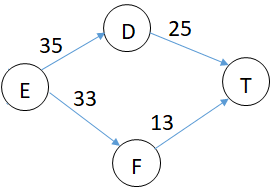
\includegraphics[align=t, width=36mm]{gafo dirigido.png} } &
%\multicolumn{1}{|l|}{Dirigido}    & \multicolumn{1}{l|}{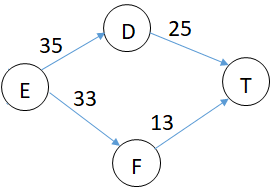
\includegraphics[width=27mm]{gafo dirigido.png} } &
\multicolumn{1}{p{6cm}|}{Todas sus aristas están dirigidas (flechas), que se pueden representar por parejas ordenadas (x,y)}     \\ \hline
\multicolumn{1}{|l|}{No dirigido} & \multicolumn{1}{l|}{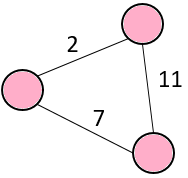
\includegraphics[align=t,width=36mm]{gafo no dirigido.png}} & \multicolumn{1}{p{6cm}|}{Todas sus aristas son no dirigidas (líneas), que se pueden representar por parejas no ordenadas \{x,y\}} \\ \hline
\multicolumn{1}{|l|}{Mixto}       & \multicolumn{1}{l|}{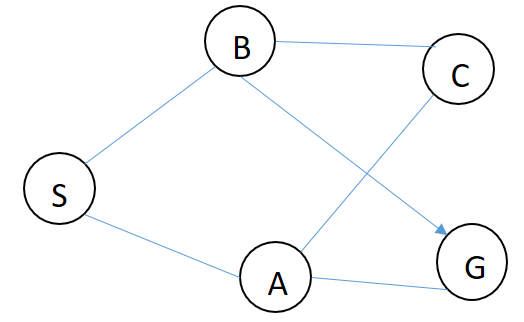
\includegraphics[align=t,width=36mm]{elementos de un grafo.png}} & \multicolumn{1}{p{6cm}|}{Contiene aristas dirigidas y aristas no dirigidas} \\ \hline
\end{tabular}
\label{dirigido}
\end{table}

Además, matemáticamente se hace una distinción en la representación de sus aristas, usándose parejas ordenas $(x,y) \in NxN$ para las aristas dirigidas y ${x,y} | (x,y) \in NxN$ para las aristas no dirigidas, lo que se puede interpretar como una doble flecha $(x,y)$ y $(y,x)$. Así que el contenido de la columna ARISTAS de la tabla \ref{tab:notgraf}, se refiere específicamente a aristas dirigidas \citep{tremblay1996matematica}.

También se habla de grafos completos, cuando contiene todas sus aristas posibles. Es decir, cada nodo tiene una arista para conectarse con cada uno de los demás existentes en el grafo. A medida que se aumenta el número de nodos en un grafo completa, su número de aristas aumenta en un progresión aritmética, porque se suma primero una, luego dos, luego tres, etc., siendo la cantidad que se suma inferior al número de nodos en una unidad, como se aprecia en la tabla \ref{cmpletos}

\begin{table}[H]
\centering
\caption{Los cinco primeros grafos completos}
\begin{tabular}[c]{|c|c|c|}
\hline
\textbf{Cantidad de nodos} & \textbf{Vista gráfica} & \textbf{Cantidad de aristas} \\ \hline
1 & \multicolumn{1}{l|}{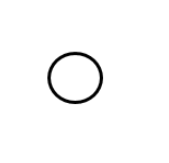
\includegraphics[align=t, width=27mm]{1nodo.png} }  & 0 \\ \hline
2 & \multicolumn{1}{l|}{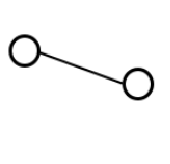
\includegraphics[align=t, width=27mm]{2nodos.png} }  & 1\\ \hline
3 & \multicolumn{1}{l|}{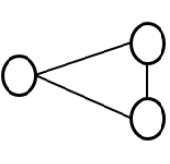
\includegraphics[align=t, width=27mm]{3nodos.png} }  & 3 \\ \hline
4 & \multicolumn{1}{l|}{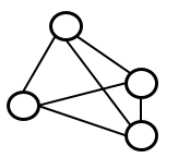
\includegraphics[align=t, width=27mm]{4nodos.png} }  & 6 \\ \hline
5 & \multicolumn{1}{l|}{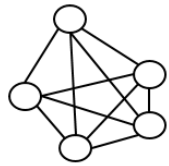
\includegraphics[align=t, width=27mm]{5nodos.png} }  & 10 \\ \hline
\end{tabular}
\label{cmpletos}
\end{table}

\section{Aprendizaje automático}
El Aprendizaje de Automático es una de las áreas de la Inteligencia Artificial que ha permitido extraer una importante cantidad de información, desde los datos que cada día se manejan en los negocios y en el mundo en general. Estos trabajos se han apoyado en diferentes técnicas como las redes Neuronales, los Algoritmos Genéticos, las Colonias de Hormigas, el Soporte de Máquina Vectorial y el Aprendizaje por Refuerzo, entre otras. En la tabla \ref{tipoML} se resume esta clasificación.

\begin{table}[H]
\caption{Tipos de aprendizaje automático}
\centering
\begin{tabular}{lc}
\multicolumn{1}{c}{\textbf{APRENDIZAJE}} & \textbf{CARACTERÍSTICA}                         \\ \hline
\multicolumn{1}{|l|}{Supervisado}        & \multicolumn{1}{c|}{Con datos de entrenamiento} \\ \hline
\multicolumn{1}{|l|}{No supervisado}     & \multicolumn{1}{c|}{Sin datos de entrenamiento} \\ \hline
\multicolumn{1}{|l|}{Por refuerzo}       & \multicolumn{1}{c|}{Premio o castigo}           \\ \hline
\end{tabular}
\label{tipoML}
\end{table}

El ML se encuentra catalogado en los textos como: aprendizaje supervisado, no supervisado o mixto, aunque el AR no se encuentra realmente en ninguna de estos tipos \citep{russell2004inteligencia}. 

En el aprendizaje supervisado el modelo aprende de acuerdo a unos datos de entrenamiento y posteriormente es capaz de reconocer patrones similares, mientras que, el aprendizaje no supervisado, no cuenta con datos de entrenamiento, sino que descubre automáticamente las características de los datos, logrando establecer, por ejemplo, las clases en las que pueden agruparse.

El AR se emplea en situaciones donde hay que tomar decisiones bajo incertidumbre, donde solo se conoce la consecuencia de una decisión, después de haberse tomado. Aquí se trata de entrenar un agente inteligente, el cual debe escoger la política que mejor resultado le dé, de acuerdo a las recompensas que recibirá de un ambiente donde se encuentra inmerso \citep{sutton1992reinforcement}.

\subsection{Los Bandits}
\label{Los Bandits}

El Multiarmed-Bandit es un modelo inspirado en las máquinas de un casino que se conocen con este nombre, donde se tienen cierto número de brazos, de los que se espera jugar los que mejor resultado alcancen y en el orden más adecuado. Cada máquina tiene su propia distribución de probabilidad, el jugador no las conoce inicialmente, pero a medida que va jugando, se va dando cuenta del resultado y va aprendiendo.

El modelo básico es el \textit{armed-bandit}, también conocido como \textit{bandit}, cuya analogía corresponde a una máquina de casino con un solo brazo o palanca, que en adelante se llamará acción. Para este modelo se tienen fórmulas sencillas que facilitan su implementación.

Por ejemplo, el beneficio acumulado que se recibe al seleccionar una acción “a” en diferentes tiempos i, es un promedio sencillo de las recompensas que el ambiente le reconoce al autómata al seleccionar dicha acción “a”, recompensa que no necesariamente será la misma en cualquier otra oportunidad o tiempo. La fórmula que se emplea es la fórmula \ref{Q}.
\begin{eqnarray}\label{Q}
Q_t(a) = \frac{R_1+R_2+ ...+R_{Nt(a)}}{N_t(a)}
\end{eqnarray}

Esta recompensa acumulada para cada acción, será afectada durante el aprendizaje del autómata y, la actividad que cuente con el mayor valor en su recompensa será la seleccionada o recomendada por el autómata o la aplicación.

El algoritmo de aprendizaje de los \textit{bandit}, es conocido como el algoritmo \textit{Q-learning}, el cual se explica en la figura \ref{AlgQ}.

\begin{figure}
  \centering
    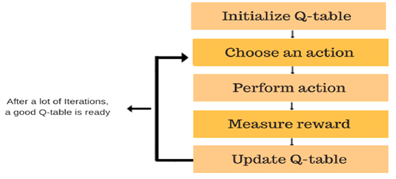
\includegraphics{Qlearning}
  \caption{Algoritmo \textit{Q-learning}. Fuente: \citep{ADL2018}}
  \label{AlgQ}
\end{figure}

Aquí \textit{Q-table}, se puede inicializar en cero para las recompensas de cada acción y se irá actualizando en forma recursiva, basándose en los valores futuros de la tabla, como se hace en programación dinámica, involucrando, por supuesto, la recompensa que el ambiente dará por la selección de la acción. De acuerdo al problema uno de estos dos valores tendrá mayor importancia: la recompensa futura o la actual, por lo que se cuenta con una variable que dará mayor peso a alguna de las dos, llamada $\gamma$, como se muestra en la fórmula \ref{Qsa}.
\begin{eqnarray}\label{Qsa} 
Q(s_t, a_t) = r(s_t, a_t) + \gamma max a_{t+1} Q(s_{t+1}, a_{t+1})
\end{eqnarray}

También implementa la estrategia $\epsilon$-greedy. El nombre de la estrategia obedece a que se cuenta con un parámetro $\epsilon$ con valores entre cero y uno, que le indicarán al agente si explota los valores de recompensa que está generando la acción que ha seleccionado o si mejor explota alguna de las otras acciones, de forma que evita que el agente se quede en la primera acción que le parezca buena, dando posibilidad a otras acciones. 

Al inicio el parámetro $\epsilon$ dará mayor importancia a la exploración, puesto que el agente no conoce todo el ambiente, y a medida que lo va conociendo le dará mayor peso a la exploración de la acción que ha selección porque ha encontrado mejores resultados, no sin dejar del todo la posibilidad de explorar otras acciones \cite{bubeck2012regret}.

%
%
De la revisión bibliográfica:

\begin{table}[H] 
\caption{Revisión de literatura - Grafos}
\centering
\begin{tabular}{cc}
\textbf{FUENTE}   & \textbf{DESCRIPCIÓN}   \\ \hline
\multicolumn{1}{|l|}{\citet{zhou2019toward}} & \multicolumn{1}{p{10cm}|}{Proponen mejoras a algoritmos de enrutamiento de ruta más corta (SPR), mediante sondeos de rutas múltiples y aprendizaje colaborativo.} \\ \hline
\multicolumn{1}{|l|}{\citet{liu2011multi}}   & \multicolumn{1}{p{10cm}|}{Recomendar la mejor ruta en un grafo, desde un origen hasta un destino donde el costo de cada enlace individual no se puede ver y el costo total de extremo a extremo solo se puede observar al finalizar el recorrido y está dado por la suma de los costos de todos los enlaces en la ruta. No hay etapas con nodos disyuntos.} \\ \hline
\multicolumn{1}{|l|}{\citet{liu2012adaptive}}   & \multicolumn{1}{p{10cm}|}{Aplican los principios del Bandido Multi-Brazos con brazos independientes al problema presentado por \citet{liu2011multi}} \\ \hline
\multicolumn{1}{|l|}{\citet{AvilaCartes2018}}   & \multicolumn{1}{p{10cm}|}{Problema \textit{Online Shortest Path Problem}, donde se usa un grafo dirigido y sin ciclos, con un nodo inicial y uno final o nodo sumidero. Haciendo uso de \textit{n-armed.bandit}, además de minimizar el costo con el camino que se seleccione, se desea disminuir la cantidad de veces que se escoge uno que presente fallas.} \\ \hline
\multicolumn{1}{|l|}{\citet{valko2016bandits}}   & \multicolumn{1}{p{10cm}|}{Recoge problemas de aplicación de grafos y \textit{bandits}, mostrando la aplicación de modelos que investigadores han desarrollado en problemas reales} \\ \hline
\multicolumn{1}{|l|}{\citet{tossou2017thompson}}   & \multicolumn{1}{p{10cm}|}{Algoritmo para problemas de decisión secuenciales, con grafos que presentan altos grados de incertidumbre, como alternativa para cuando las decisiones se tomaban basados en sencillos cálculos de probabilidades, quedando uno de dos eventos aceptado y el otro descartado.} \\ \hline
\end{tabular}
\label{tab:litera}
\end{table}

\begin{table}[H] 
\caption{Revisión de literatura - Aprendizaje por refuerzo}
\centering
\begin{tabular}{cc}
\textbf{FUENTE}   & \textbf{DESCRIPCIÓN}   \\ \hline
\multicolumn{1}{|l|}{\citet{lee2005reinforcement}} & \multicolumn{1}{p{10cm}|}{Propuesta para mejorar el tiempo de decisión de un algoritmo \textit{AQ-learnig} de aprendizaje por refuerzo con técnicas de inteligencia artificial de búsqueda por colonia de hormigas.} \\ \hline
\multicolumn{1}{|l|}{\citet{alon2017nonstochastic}}   & \multicolumn{1}{p{10cm}|}{Mediante los principios de Regresión, crean un espectro de modelos cuya complejidad está entre la de los problemas donde el agente conoce únicamente la recompensa de las acciones luego de elegirlas, y la de aquellos donde el agente tiene la información de lo que ocurrirá con cualquier acción candidata en cualquier instante.} \\ \hline
\multicolumn{1}{|l|}{\citet{alon2015online}}   & \multicolumn{1}{p{10cm}|}{Modelan el problema de un jugador aleatorio que se encuentra dentro de un ambiente que puede ser su adversario, quien después de cada acción recibe de sus vecinos información binaria del efecto de su acción.} \\ \hline
\multicolumn{1}{|l|}{\citet{gokcesu2018online}}   & \multicolumn{1}{p{10cm}|}{Presentan un algoritmo para \textit{n-armed bandits} con complejidad lineal que crece en función de la cantidad de secuencias posibles y del número de rondas del juego, sin el conocimiento del brazo que se debería escoger y sin suposiciones estadísticas.} \\ \hline
\multicolumn{1}{|l|}{\citet{8170860}}   & \multicolumn{1}{p{10cm}|}{Modelado de un problema de aprendizaje por refuerzo, mediante grafos, con un grafo en el que los nodos sí representan los brazos, pero las aristas tiene que ver con la similitud de sus valores de recompensas, aplicable a los sistemas de recomendación con baja complejidad} \\ \hline
\multicolumn{1}{|p{4cm}|}{\citet{silver2017mastering} y \citet{silver2016mastering}}   & \multicolumn{1}{p{10cm}|}{Aplicación de técnicas de aprendizaje por refuerzo para el entrenamiento de redes neuronales que lograron derrotar a los mejores jugadores humanos de ajedrez y Go, entre otros juegos, cada vez, con mejores resultados.} \\ \hline
\end{tabular}
\label{tab:litera}
\end{table}



\chapter{FUNDAMENTOS}
\label{chap:Mt}
%\section{FUNDAMENTO TEÓRICO} 
Se dedica este capítulo a exponer los conceptos necesarios para entender el problema de investigación que se aborda.

\section{Conceptos básicos y antecedentes}

En este aparte se presentan algunos conceptos que puedes ser básicos, pero que permiten la contextualización del problema de esta tesis, así como un resumen de las publicaciones que soportar esta investigación y su aplicación en el problema que se aborda.

Preferiblemente se tomaron las referencias de los últimos 5 años, pero no se descartan otras que son básicas en este campo de investigación.

\subsection{Conceptos básicos de Grafos}
\label{ConcepGraph}
Un grafo no es otra cosa que un conjunto de vértices (al menos uno) conectados entre ellos con aristas que pueden ser líneas o flechas. 

Los grafos pueden ser dirigidos o no dirigidos, lo que gráficamente significa que sus aristas son flechas o líneas, respectivamente; si hay de ambas, se llaman grafos mixtos, como se aprecia en la tabla \ref{dirigido}.

\begin{table}[H]
\caption{Clasificación de grafos según sus aristas}
\centering
\begin{tabular}[c]{lcc}
\multicolumn{1}{c}{\textbf{TIPO}} & \textbf{DIBUJO}                      & \textbf{CARACTERÍSTICA}  \\ \hline
\multicolumn{1}{|l|}{Dirigido}    & \multicolumn{1}{l|}{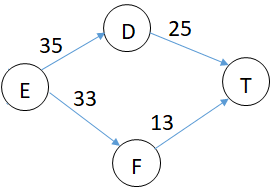
\includegraphics[align=t, width=36mm]{gafo dirigido.png} } &
%\multicolumn{1}{|l|}{Dirigido}    & \multicolumn{1}{l|}{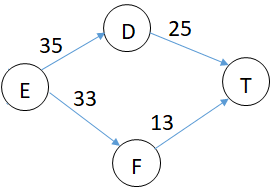
\includegraphics[width=27mm]{gafo dirigido.png} } &
\multicolumn{1}{p{6cm}|}{Todas sus aristas están dirigidas (flechas), que se pueden representar por parejas ordenadas (x,y)}     \\ \hline
\multicolumn{1}{|l|}{No dirigido} & \multicolumn{1}{l|}{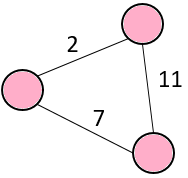
\includegraphics[align=t,width=36mm]{gafo no dirigido.png}} & \multicolumn{1}{p{6cm}|}{Todas sus aristas son no dirigidas (líneas), que se pueden representar por parejas no ordenadas \{x,y\}} \\ \hline
\multicolumn{1}{|l|}{Mixto}       & \multicolumn{1}{l|}{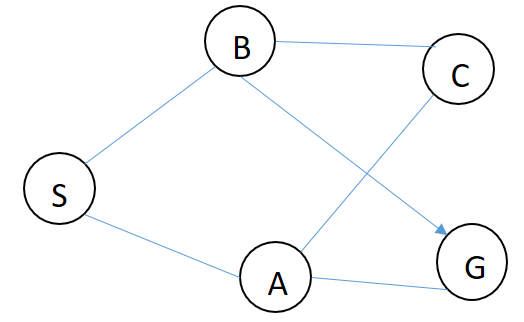
\includegraphics[align=t,width=36mm]{elementos de un grafo.png}} & \multicolumn{1}{p{6cm}|}{Contiene aristas dirigidas y aristas no dirigidas} \\ \hline
\end{tabular}
\label{dirigido}
\end{table}

Además, matemáticamente se hace una distinción en la representación de sus aristas, usándose parejas ordenas $(x,y) \in NxN$ para las aristas dirigidas y ${x,y} | (x,y) \in NxN$ para las aristas no dirigidas, lo que se puede interpretar como una doble flecha $(x,y)$ y $(y,x)$ \citep{tremblay1996matematica}.

También se habla de grafos conexos cuando no se puede separar en componentes o partes entre las que no aparecen aristas que las conecten, es decir que cada par de nodos debe estar conectado mediante un secuencia de aristas o mediante un camino.

Los grafos bipartitos son aquellos en los que se pueden diferenciar claramente dos grupos de nodos; en cada grupo de nodos no se encuentran aristas que los conecte, sino que estas van un nodo de un grupo al otro. Estos y otros conceptos sobre grafos se pueden ampliar en \citep{brandstadt1999graph}.

Estas características se cumplen en el grafo que se propone en esta tesis, además de una característica propia que se ha denominado <<grafo por etapas>>, la cual consiste en que el grafo cuenta con sus nodos distribuidos en $L$ etapas claramente diferenciadas, de forma similar a los grafos bipartitos, pero con más de dos grupos de nodos.

Esta estructura por etapas facilita el recorrido estocástico desde la primera hasta la última etapa, en orden y con probabilidades asociadas a las conexiones entre nodos, que se prestan para realizar búsquedas en el grafo, basadas en muestreo.

\subsection{Aprendizaje automático}
El Aprendizaje de Automático es una de las áreas de la Inteligencia Artificial que ha permitido extraer una importante cantidad de información, a partir de los datos que cada día se manejan en los negocios y en el mundo en general. Algunos trabajos, en este sentido, se han apoyado en diferentes técnicas como las redes Neuronales, los Algoritmos Genéticos, las Colonias de Hormigas, el Soporte de Máquina Vectorial y el Aprendizaje por Refuerzo, entre otras. 


El Aprendizaje automático se encuentra catalogado en los textos como: aprendizaje supervisado, no supervisado o mixto, aunque el aprendizaje por refuerzo - AR no se encuentra realmente en ninguna de estos tipos \citep{russell2004inteligencia}. En la tabla \ref{tipoML} se resume esta clasificación.

\begin{table}[H]
\caption{Tipos de aprendizaje automático}
\centering
\begin{tabular}{lc}
\multicolumn{1}{c}{\textbf{APRENDIZAJE}} & \textbf{CARACTERÍSTICA}                         \\ \hline
\multicolumn{1}{|l|}{Supervisado}        & \multicolumn{1}{c|}{Con datos de entrenamiento} \\ \hline
\multicolumn{1}{|l|}{No supervisado}     & \multicolumn{1}{c|}{Sin datos de entrenamiento} \\ \hline
\multicolumn{1}{|l|}{Por refuerzo}       & \multicolumn{1}{c|}{Premio o castigo}           \\ \hline
\end{tabular}
\label{tipoML}
\end{table}


En el aprendizaje supervisado el modelo aprende de acuerdo a unos datos de entrenamiento y posteriormente es capaz de reconocer patrones similares, mientras que, el aprendizaje no supervisado, no cuenta con datos de entrenamiento, sino que descubre automáticamente las características de los datos, logrando establecer, por ejemplo, las clases en las que pueden agruparse.

El AR se emplea en situaciones donde hay que tomar decisiones bajo incertidumbre, donde solo se conoce la consecuencia de una decisión después de haberla tomado. Aquí se trata de entrenar un agente inteligente, el cual debe escoger la política que mejor resultado le dé, de acuerdo a las recompensas que recibirá de un ambiente donde se encuentra inmerso \citep{sutton1992reinforcement}.

\subsection{Los Bandits}
\label{Los Bandits}

El Multiarmed-Bandit o \textit{n-armed bandits} es un modelo inspirado en las máquinas de un casino que se conocen con este nombre, donde se tienen cierto número de brazos, de los que se espera jugar los que mejor resultado alcancen. Cada máquina tiene su propia distribución de probabilidad; el jugador no las conoce inicialmente, pero a medida que va jugando, se va dando cuenta del resultado y va aprendiendo.

El modelo básico es el \textit{armed-bandit}, también conocido como \textit{bandit}, concepto que se utiliza en esta tesis, cuya analogía corresponde a una máquina de casino con un solo brazo o palanca, que en adelante se llamará acción. Para este modelo se tienen fórmulas sencillas que facilitan su implementación. 

Por ejemplo, el valor que tendrá seleccionar una acción $a$ en el tiempo $t$ se estima mediante un promedio sencillo de las recompensas que el autómata ha recibido del ambiente cada vez que seleccionó dicha acción $a$, recompensa que no necesariamente será la misma en cualquier otra oportunidad o tiempo. La fórmula que se emplea es la \ref{Q}, donde $R_i$ son los valores de recompensa que va recibiendo el autómata en cada una de las $Nt(a)$ ocasiones en que la acción $a$ fue seleccionada.
\begin{eqnarray}\label{Q}
Q_t(a) = \frac{R_1+R_2+ ...+R_{Nt(a)}}{N_t(a)}
\end{eqnarray}

Este valor asociado a cada acción, será actualizado durante el aprendizaje del autómata, es decir que para cada tiempo $t$ puede cambiar y, de él depende que la acción tenga mayor posibilidad de ser seleccionada por el autómata en ese momento, de acuerdo a lo que muestra la figura \ref{A} \citep{sutton1998introduction}.
\begin{eqnarray}\label{A}
A_t = \stackbin[a]{}{arg max}Q_t(a)
\end{eqnarray}

Así, no es completamente seguro que la acción con mejor valor sea escogida, porque estos algoritmos, y en general los del AR, hacen un balance entre la exploración y la explotación y el agente deberá decidir entre elegir acciones que ya sabe que dan un buen resultado o acciones que no ha probado o que en el pasado, no han sido las mejores; en el primer caso, para mejorar la recompensa que esa acción le ofrece y, en el segundo caso, para darse la oportunidad de encontrar acciones con mejor recompensa \citep{sutton1992reinforcement}. Una analogía de estos procesos es la búsqueda de un valor óptimo en una función; en el primer caso el agente se quedaría explorando un óptimo local y, en el segundo caso exploraría otros lugares de la función donde puede que aparezca el óptimo global.

\subsection{Antecedentes sobre Grafos}
Diferentes investigadores han propuesto aplicaciones de grafos en problemas particulares, así como la mejora o adaptación de algoritmos ya existentes.

Entre ellos, \citet{zhou2019toward} proponen mejoras a algoritmos de enrutamiento de ruta más corta (Shortest Path Routing - SPR), mediante sondeos de rutas múltiples y aprendizaje colaborativo. Citan, además, trabajos en esta misma área como el de \citet{liu2012adaptive} quienes aplican los principios del Bandido Multi-Brazos con brazos independientes, al problema presentado por \citet{liu2011multi}, quienes pretenden recomendar la mejor ruta en un grafo, desde un origen hasta un destino, donde el costo de cada enlace individual no se puede ver y el costo total de extremo a extremo solo se puede observar al finalizar el recorrido y está dado por la suma de los costos de todos los enlaces en la ruta. 

Un problema similar, conocido como \textit{Online Shortest Path Problem}, es abordado como trabajo de grado por \citet{AvilaCartes2018}, mediante el uso de un grafo dirigido y sin ciclos, con un nodo inicial y uno final o nodo sumidero. La solución aprovecha los alcances del \textit{n-armed.bandit}, pero, además de minimizar el costo con el camino que se seleccione, busca disminuir la cantidad de veces que se escoge uno que presente fallas.

Otra tesis donde se recogen problemas de aplicación de grafos y \textit{bandits}, es la de \citet{valko2016bandits} quien se esfuerza por mostrar la aplicación de modelos que investigadores han desarrollado en problemas reales, valiéndose de los grafos y cómo hacer uso de los desarrollos en \textit{n-armed-bandit}.

Es el caso de \cite{tossou2017thompson}, ellos proponen un algoritmo para problemas de decisión secuenciales, con grafos que presentan altos grados de incertidumbre, basado en los enunciados de \citet{thompson1933likelihood}, como alternativa para las decisiones que se toman basados en sencillos cálculos de probabilidades, donde uno de dos eventos queda aceptado y el otro descartado. 

Se cita también una propuesta de investigadores en inteligencia artificial de IBM \citep{lakshmanan2010predictive} que modelan un caso semiestructurado de Gestión de Procesos de Negocios, mediante un grafo cuyos nodos son las actividades y sus aristas indica si hay flujo entre cada par de nodos. Se tiene la información de quienes son los vecinos de cada nodo y una probabilidad de pasar a cada uno de ellos, las cuales deben sumar 1; estas son las probabilidades que la aplicación va a ir modificando hasta encontrar una sola secuencia de actividades para dar solución al caso; dicha modificación sigue las reglas de las feromonas de los algoritmos de Optimización con Colonia de Hormigas para encontrar cuál nodo ha de recibir la recompensa y para actualizar todas las probabilidades de acceder a los vecinos de un nodo. A medida que van disminuyendo los valores de las probabilidades para algunas aristas, también llegará el momento en que algunos nodos ya no sean tenidos en cuenta.

En este trabajo como en otros, el grafo propuesto no implica mayores características que ser un grafo conexo y dirigido, con un nodo origen y un nodo final establecidos, sin encontrar en dichos trabajos las características del grafo por etapas, objeto de esta tesis. 

Un resumen de esta revisión bibliográfica se presenta en la tabla \ref{tab:litera1}
\begin{table}[h] 
\caption{Revisión de literatura - Grafos}
\centering
\begin{tabular}{cc}
\textbf{FUENTE}   & \textbf{DESCRIPCIÓN}   \\ \hline
\multicolumn{1}{|l|}{\citet{zhou2019toward}} & \multicolumn{1}{p{10cm}|}{Proponen mejoras a algoritmos de enrutamiento de ruta más corta (SPR), mediante sondeos de rutas múltiples y aprendizaje colaborativo.} \\ \hline
\multicolumn{1}{|l|}{\citet{liu2011multi}}   & \multicolumn{1}{p{10cm}|}{Recomendar la mejor ruta en un grafo, desde un origen hasta un destino donde el costo de cada enlace individual no se puede ver y el costo total de extremo a extremo solo se puede observar al finalizar el recorrido y está dado por la suma de los costos de todos los enlaces en la ruta. No hay etapas con nodos disyuntos.} \\ \hline
\multicolumn{1}{|l|}{\citet{liu2012adaptive}}   & \multicolumn{1}{p{10cm}|}{Aplican los principios del Bandido Multi-Brazos con brazos independientes al problema presentado por \citet{liu2011multi}} \\ \hline
\multicolumn{1}{|l|}{\citet{AvilaCartes2018}}   & \multicolumn{1}{p{10cm}|}{Problema \textit{Online Shortest Path Problem}, donde se usa un grafo dirigido y sin ciclos, con un nodo inicial y uno final o nodo sumidero. Haciendo uso de \textit{n-armed.bandit}, además de minimizar el costo con el camino que se seleccione, se desea disminuir la cantidad de veces que se escoge uno que presente fallas.} \\ \hline
\multicolumn{1}{|l|}{\citet{valko2016bandits}}   & \multicolumn{1}{p{10cm}|}{Recoge problemas de aplicación de grafos y \textit{bandits}, mostrando la aplicación de modelos que investigadores han desarrollado en problemas reales} \\ \hline
\multicolumn{1}{|l|}{\citet{tossou2017thompson}}   & \multicolumn{1}{p{10cm}|}{Algoritmo para problemas de decisión secuenciales, con grafos que presentan altos grados de incertidumbre, como alternativa para cuando las decisiones se tomaban basados en sencillos cálculos de probabilidades, quedando uno de dos eventos aceptado y el otro descartado.} \\ \hline
\end{tabular}
\label{tab:litera1}
\end{table}

%Se exploró entonces la aplicación que se ha hecho de \textit{bandits} en problemas modelados por grafos, encontrando que muchos de ellos han aportado a los actuales modelos de toma de decisiones llamados sistemas de recomendación.
\subsection{Antecedentes sobre aprendizaje por refuerzo}
Muchas investigaciones se han dado para mejorar o adaptar los métodos de aprendizaje por refuerzo a diferentes situaciones.

Una propuesta para mejorar el tiempo de decisión de un algoritmo \textit{AQ-learnig} de aprendizaje por refuerzo con técnicas de inteligencia artificial de búsqueda por colonia de hormigas, se puede consultar en \citep{lee2005reinforcement}.

Se encuentra también la propuesta de \citet{alon2017nonstochastic}, quienes, mediante los principios de Regresión, crean un espectro de modelos cuya complejidad está entre la de los problemas donde el agente conoce únicamente la recompensa de las acciones luego de que las va eligiendo, y la de los problemas donde el agente tiene la información de lo que ocurrirá con cualquier acción candidata en cualquier instante de tiempo.

De otra parte, \citet{alon2015online} modelan el problema de un jugador aleatorio que se encuentra dentro de un ambiente adversario, de forma que después de cada acción, el jugador recibe de sus vecinos información binaria del efecto de su acción, que le permitirá mejorar sus próximas decisiones.

\citet{gokcesu2018online} presentan un algoritmo para \textit{n-armed bandits} con complejidad lineal que crece en función de la cantidad de secuencias posibles y del número de rondas del juego, sin el conocimiento del brazo que se debería escoger y sin suposiciones estadísticas.

Así mismo, en \citep{8170860} se encuentra un modelado de un problema de aprendizaje por refuerzo, mediante grafos, no con el esquema tradicional de la secuencia de los brazos seleccionado, sino que es un grafo en el que los nodos sí representan los brazos, pero las aristas tiene que ver con la similitud de sus valores de recompensas, lo que es aplicable a los sistemas de recomendación. El modelo les permitió presentar un algoritmo con baja complejidad. 

Como \citet{alon2017nonstochastic} y \citet{xu2017online}, muchos autores han hecho propuestas para mejorar el desempeño de algoritmos existentes, en cuanto a su complejidad o al campo de solución que influyen, utilizando técnicas de aprendizaje por refuerzo en el escenario de los \textit{bandits}. En general, se trabaja con un \textit{m-armed bandit}, donde los nodos representan los brazos y, las aristas, dirigidas o no dirigidas, relacionan los nodos.

Y, finalmente, no se puede dejar de mencionar el trabajo de \citet{silver2017mastering} y los predecesores de \textit{AlphaZero} \citep{silver2016mastering} que revolucionaron al mundo con la aplicación de técnicas de aprendizaje por refuerzo para mejorar el entrenamiento conseguido con redes neuronales de aprendizaje profundo, que logró derrotar a los mejores jugadores humanos de ajedrez y Go, entre otros juegos, cada vez con mejores resultados.

De esta forma se puede apreciar que en la revisión hecha, no se encuentra una propuesta que combine los aspectos del aprendizaje por refuerzo de los \textit{m-armed bandit}, con un grafo que tenga como restricción que la acción seguida a ejecutar deba pertenecer a la etapa siguiente de la anterior, como lo contempla la propuesta de esta tesis.
%\section{Gestión de Procesos de Negocio}

Un resumen de esta revisión bibliográfica se presenta en la tabla \ref{tab:litera2}

\begin{table}[!h] 
\caption{Revisión de literatura - Aprendizaje por refuerzo}
\centering
\begin{tabular}{cc}
\textbf{FUENTE}   & \textbf{DESCRIPCIÓN}   \\ \hline
\multicolumn{1}{|l|}{\citet{lee2005reinforcement}} & \multicolumn{1}{p{10cm}|}{Propuesta para mejorar el tiempo de decisión de un algoritmo \textit{AQ-learnig} de aprendizaje por refuerzo con técnicas de inteligencia artificial de búsqueda por colonia de hormigas.} \\ \hline
\multicolumn{1}{|l|}{\citet{alon2017nonstochastic}}   & \multicolumn{1}{p{10cm}|}{Mediante los principios de Regresión, crean un espectro de modelos cuya complejidad está entre la de los problemas donde el agente conoce únicamente la recompensa de las acciones luego de elegirlas, y la de aquellos donde el agente tiene la información de lo que ocurrirá con cualquier acción candidata en cualquier instante.} \\ \hline
\multicolumn{1}{|l|}{\citet{alon2015online}}   & \multicolumn{1}{p{10cm}|}{Modelan el problema de un jugador aleatorio que se encuentra dentro de un ambiente que puede ser su adversario, quien después de cada acción recibe de sus vecinos información binaria del efecto de su acción.} \\ \hline
\multicolumn{1}{|l|}{\citet{gokcesu2018online}}   & \multicolumn{1}{p{10cm}|}{Presentan un algoritmo para \textit{n-armed bandits} con complejidad lineal que crece en función de la cantidad de secuencias posibles y del número de rondas del juego, sin el conocimiento del brazo que se debería escoger y sin suposiciones estadísticas.} \\ \hline
\multicolumn{1}{|l|}{\citet{8170860}}   & \multicolumn{1}{p{10cm}|}{Modelado de un problema de aprendizaje por refuerzo, mediante grafos, con un grafo en el que los nodos sí representan los brazos, pero las aristas tiene que ver con la similitud de sus valores de recompensas, aplicable a los sistemas de recomendación con baja complejidad} \\ \hline
\multicolumn{1}{|p{4cm}|}{\citet{silver2017mastering} y \citet{silver2016mastering}}   & \multicolumn{1}{p{10cm}|}{Aplicación de técnicas de aprendizaje por refuerzo y redes neuronales de aprendizaje profundo, que lograron derrotar a los mejores jugadores humanos de ajedrez y Go, entre otros juegos, cada vez, con mejores resultados.} \\ \hline
\end{tabular}
\label{tab:litera2}
\end{table}

Luego de estas revisiones se procede a describir las bases matemáticas que soportan el modelo \textit{L-n-armed-bandits}, para que se constituya en una propuesta novedosa que se sume a las muchas que se han generado para contribuir cada día a una mejor toma de decisiones, para las personas y para las aplicaciones mismas.

\section{Denominación del modelo propuesto}
\label{nombre}

\textit{El algoritmo propuesto se ha llamado \textit{L-n-armed bandit} ya que se basa en el algoritmo \textit{n-armed bandit} para un grafo por etapas (ya definido), cuya cantidad está representada por la letra $L$}

\textit{Cabe resaltar que este grafo ha de contener la cantidad de etapas $L$ que el problema a modelar requiera, así como los nodos de cada etapa y las conexiones entre nodos de etapas seguidas; sin embargo, para el desarrollo de la propuesta se generarán de forma aleatoria algunos de estos valores, cuya digitalización puede resultaría tediosa en cada una de las pruebas a que se someta.}

\textit{Esta estructura por etapas facilita el recorrido estocástico desde la primera hasta la última etapa, en orden y con probabilidades asociadas a las conexiones entre nodos, lo que se presta para realizar búsquedas en el grafo, basadas en muestreo. Para conseguir estas probabilidades se aprovecha la forma de operar del algoritmo \textit{n-armed bandit}.}

\textit{Cada uno de los nodos del grafo será en realidad un \textit{bandit} con un valor o utilidad desconocido que solo se podrá ir estimando al terminar la selección de los L nodos de todas las etapas del grafo, ya que en la última etapa es donde se recibe algún refuerzo positivo o negativo, de acuerdo al conjunto de nodos seleccionados de cada etapa.}

\textit{Las forma como se generan valores y se simulan los refuerzos, así como las bases matemática que soportan la propuesta se describen en seguida.}

\section{Fundamentos matemáticos}

Como ya se ha mencionado, se pretende usar un modelo estructurado que aproxime los valores de una matriz de probabilidades de transición de estados, que se relacionen con los valores de utilidad que en un momento dado tengan los nodos candidatos a ser visitados.

Un modelo de probabilidades de transición de estados se adapta al problemas de búsqueda en el grafo por etapas con cualquier cantidad de nodos y remplazaría la forma de seleccionar una acción que se explicó para los \textit{bandits} en las ecuaciones \ref{Q} y \ref{A} \citep{sutton1998introduction}.

También se ha de tener en cuenta que, la probabilidad total de una secuencia determinada de nodos, equivale a multiplicar las probabilidades de ir de un nodo a otro hasta culminar la ruta, tal como se hace en un árbol Bayesiano y como se presenta en la fórmula \ref{modelp1}.
\begin{eqnarray}
\label{modelp1}
P(i_{0} \to i_{1}, ... i_{l-1} \to i_{l}, ... i_{L-1} \to i_{L})=P(i_{0} \to i_{1})P(i_{1} \to i_{2})...P(i_{L-1} \to i_{L}),
\end{eqnarray}
donde $i$ denota el nodo seleccionado en cada una de las etapas, su subíndice $l=0,1,...,L$ denota la etapa a la que pertenece y L denota el número total de etapas. 

La fórmula \ref{for:2}, como sucede con la distribución de \textit{Boltzman}, permite normalizar las probabilidades para que correspondan a cantidades positivas menores o iguales a 1, pero con un fácil cálculo de la sudatoria del denominador, dados los valores de A que corresponden a ceros o a unos. 

\begin{eqnarray}\label{for:2}
P(i \to j) = \frac{e^{v_j}}{\sum_k A_{i,k} e^{v_k}},
\end{eqnarray}


Así, la cantidad del numerador siempre será inferior o,  a lo sumo, igual a la cantidad del denominador, dado que el numerado es parte de la sumatoria del denominador, que, adicionalmente, es de valores positivos. La multiplicación por el valor de cada posición en la matriz de adyacencia $A$, garantiza que únicamente se sumen los exponenciales de nodos a los que en realidad se accede. 

Otra característica de esta fórmula es que con los valores iniciales en cero para los exponentes de $e$, se obtienen probabilidades uniformes para todo nodo $j$ adyacente al nodo $i$.

Finalmente, para controlar el aprendizaje del autómata se incrementa o decrementa el valor del exponente de la fórmula anterior, dado que de esta forma aumenta o disminuye la probabilidad asociada al nodo relacionado. Esto puede verse en la fórmula sencilla \ref{for:3}.
\begin{eqnarray}\label{for:3}
v_j(\tau + 1) = v_j(\tau) + \delta,
\end{eqnarray}

donde $\delta$ es un parámetro que controla la rata de aprendizaje:

$P(i \to j)_{\tau+1} \sim e^{\delta} P(i \to j)_{\tau}$ 

para pequeños valores de $\delta$.

\section{Proceso de negocio}

Aunque la definición de proceso es algo que está en la mente de cualquiera de los lectores, se define aquí un proceso de negocio como un conjunto de actividades ejecutadas en una secuencia específica, es decir, que tiene un flujo determinado por la lógica del negocio, los eventos externos y las reglas del negocio \citep{hitpass2017bpm}, para dar un contexto inicial del contenido de este capítulo. A partir de este concepto se derivan los que aquí se exponen.

\subsection{Gestión de procesos de negocio}

BPM es el acrónimo de Business Process Management, en español: Gestión de Procesos de Negocio. Es una disciplina que integra un conjunto de principios, métodos y tecnologías con el propósito de contribuir al mejoramiento continuo del funcionamiento empresarial.

La idea de BPM es hacer visible la gestión de los procesos de negocio y facilitar los cambios que sean requeridos \citep{smith2003business}.

Según \citet{garimella2008introduccion}, BPM hace referencia a un conjunto de mejores prácticas de gestión de procesos, herramientas y tecnologías utilizadas para diseñar, representar, analizar y controlar los procesos del negocio, combinando las tecnologías de la información con metodologías de proceso y gobierno.

BPM incluye el soporte integral de las tecnologías de información para mejorar, innovar y gestionar los procesos que determinan los resultados del negocio, crean valor para el cliente y facilitan el logro ágil de los objetivos del negocio” \citep{abpmp2013v3}.

\subsubsection{Suite de gestión de procesos de negocio bpms}

Un sistema o suite para la gestión de procesos de negocios (Business Process Management Suite (BPMS) “es un conjunto de herramientas de software que permiten modelar implementar y gestionar los procesos de negocio, que abarcan múltiples aplicaciones empresariales, departamentos y \textit{partners}”\citep{smith2003business}.

Una Suite de Gestión de Procesos de Negocio está conformada por herramientas de software para la gestión de los procesos de negocios (diseño de procesos, flujo de trabajo, aplicaciones, integración y supervisión), los cuales son automatizados favoreciendo a las organizaciones \citep{underdahl2013gestion}.

\subsection{Proceso de negocio dinámico y caso}

Es un proceso de negocio que no tiene un orden determinado para la ejecución de las actividades, ni la certeza de cuáles de ellas se han de ejecutar, requiriendo la intervención de un experto \citep{hitpass2017bpmn}. 

El término \textit{case}, que en \cite{van2005case} se define como una situación que puede ocurrir en una organización, para la cual el procedimiento de resolución no está necesariamente predefinido.

A la tecnología que se encarga de la gestión de este tipo de procesos se le conoce momo gestión de “casos”; el caso contiene toda la información sobre el proceso \citep{marin2016introduction}.

%\section{Modelo y notación de procesos de negocio}

%Las notaciones BPMN y CMMN que se describen en este apartado, son grafos de actividades y otros elementos que indican la secuencia de tareas que se siguen para que la BPMS guíe el desarrollo de un proceso, este hecho es el que motiva que se puede orientar el modelo al grafo que aquí se expone, aplicando una estrategia particular que permita trasladar toda la información necesaria.

%\subsection{BPMN}

%Business Process Model and Notation (BPMN) es una herramienta gráfica estandarizada, para la notación del modelado de procesos de negocio, mediante un flujo de trabajo.

%La versión BPMN 2.0 fue presentada en el año 2011 \citep{omg2011business} y utiliza símbolos, relaciones y atributos para el modelado de procesos de negocio. Un ejemplo gráfico de cómo se ve un proceso modelado en BPMN se muestra en la figura \ref{EjBPMN}.

%Una recopilación de conceptos de modelado de procesos y los elementos que componen cada modelo, son ampliados por \citet{lemusenfoque}.

%\begin{figure}[H]
  %\centering
   % 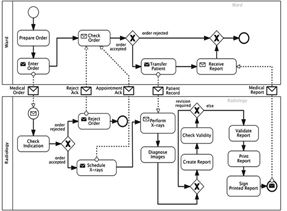
\includegraphics[scale=1.5]{EjBPMN.png}
  %\caption[Modelado de un proceso estructurado]{Modelado de un proceso estructurado con BPMN}
  %\label{EjBPMN}
%\end{figure}

\subsection{CMMN}
\label{Sec:CMMN}

Uno de los estándares emergentes para el modelado de casos es Case Management Model and Notation (CMMN), que utiliza un conjunto de símbolos gráficos, reglas de composición y artefactos para este propósito; una descripción completa de esta notación se encuentra en \cite {Cmmn}, pero se enfatiza que las líneas de puntos alrededor de las actividades las hacen opcionales y esto revela la incertidumbre que caracteriza a los casos.

Case Management Model and Notation” – CMMN es una referenciación entregada por el grupo “Object Management Group” (OMG), como una notación gráfica para la gestión de casos y procesos dinámicos \citep{hauder2014research}; algunas de sus principales diferencias con la notación de procesos de negocio deterministas se ilustra en \citet{breitenmoser2015case}. \citet{auer2014business} también fundamenta y explica la notación CMMN.

\begin{figure}[h]
  \centering
    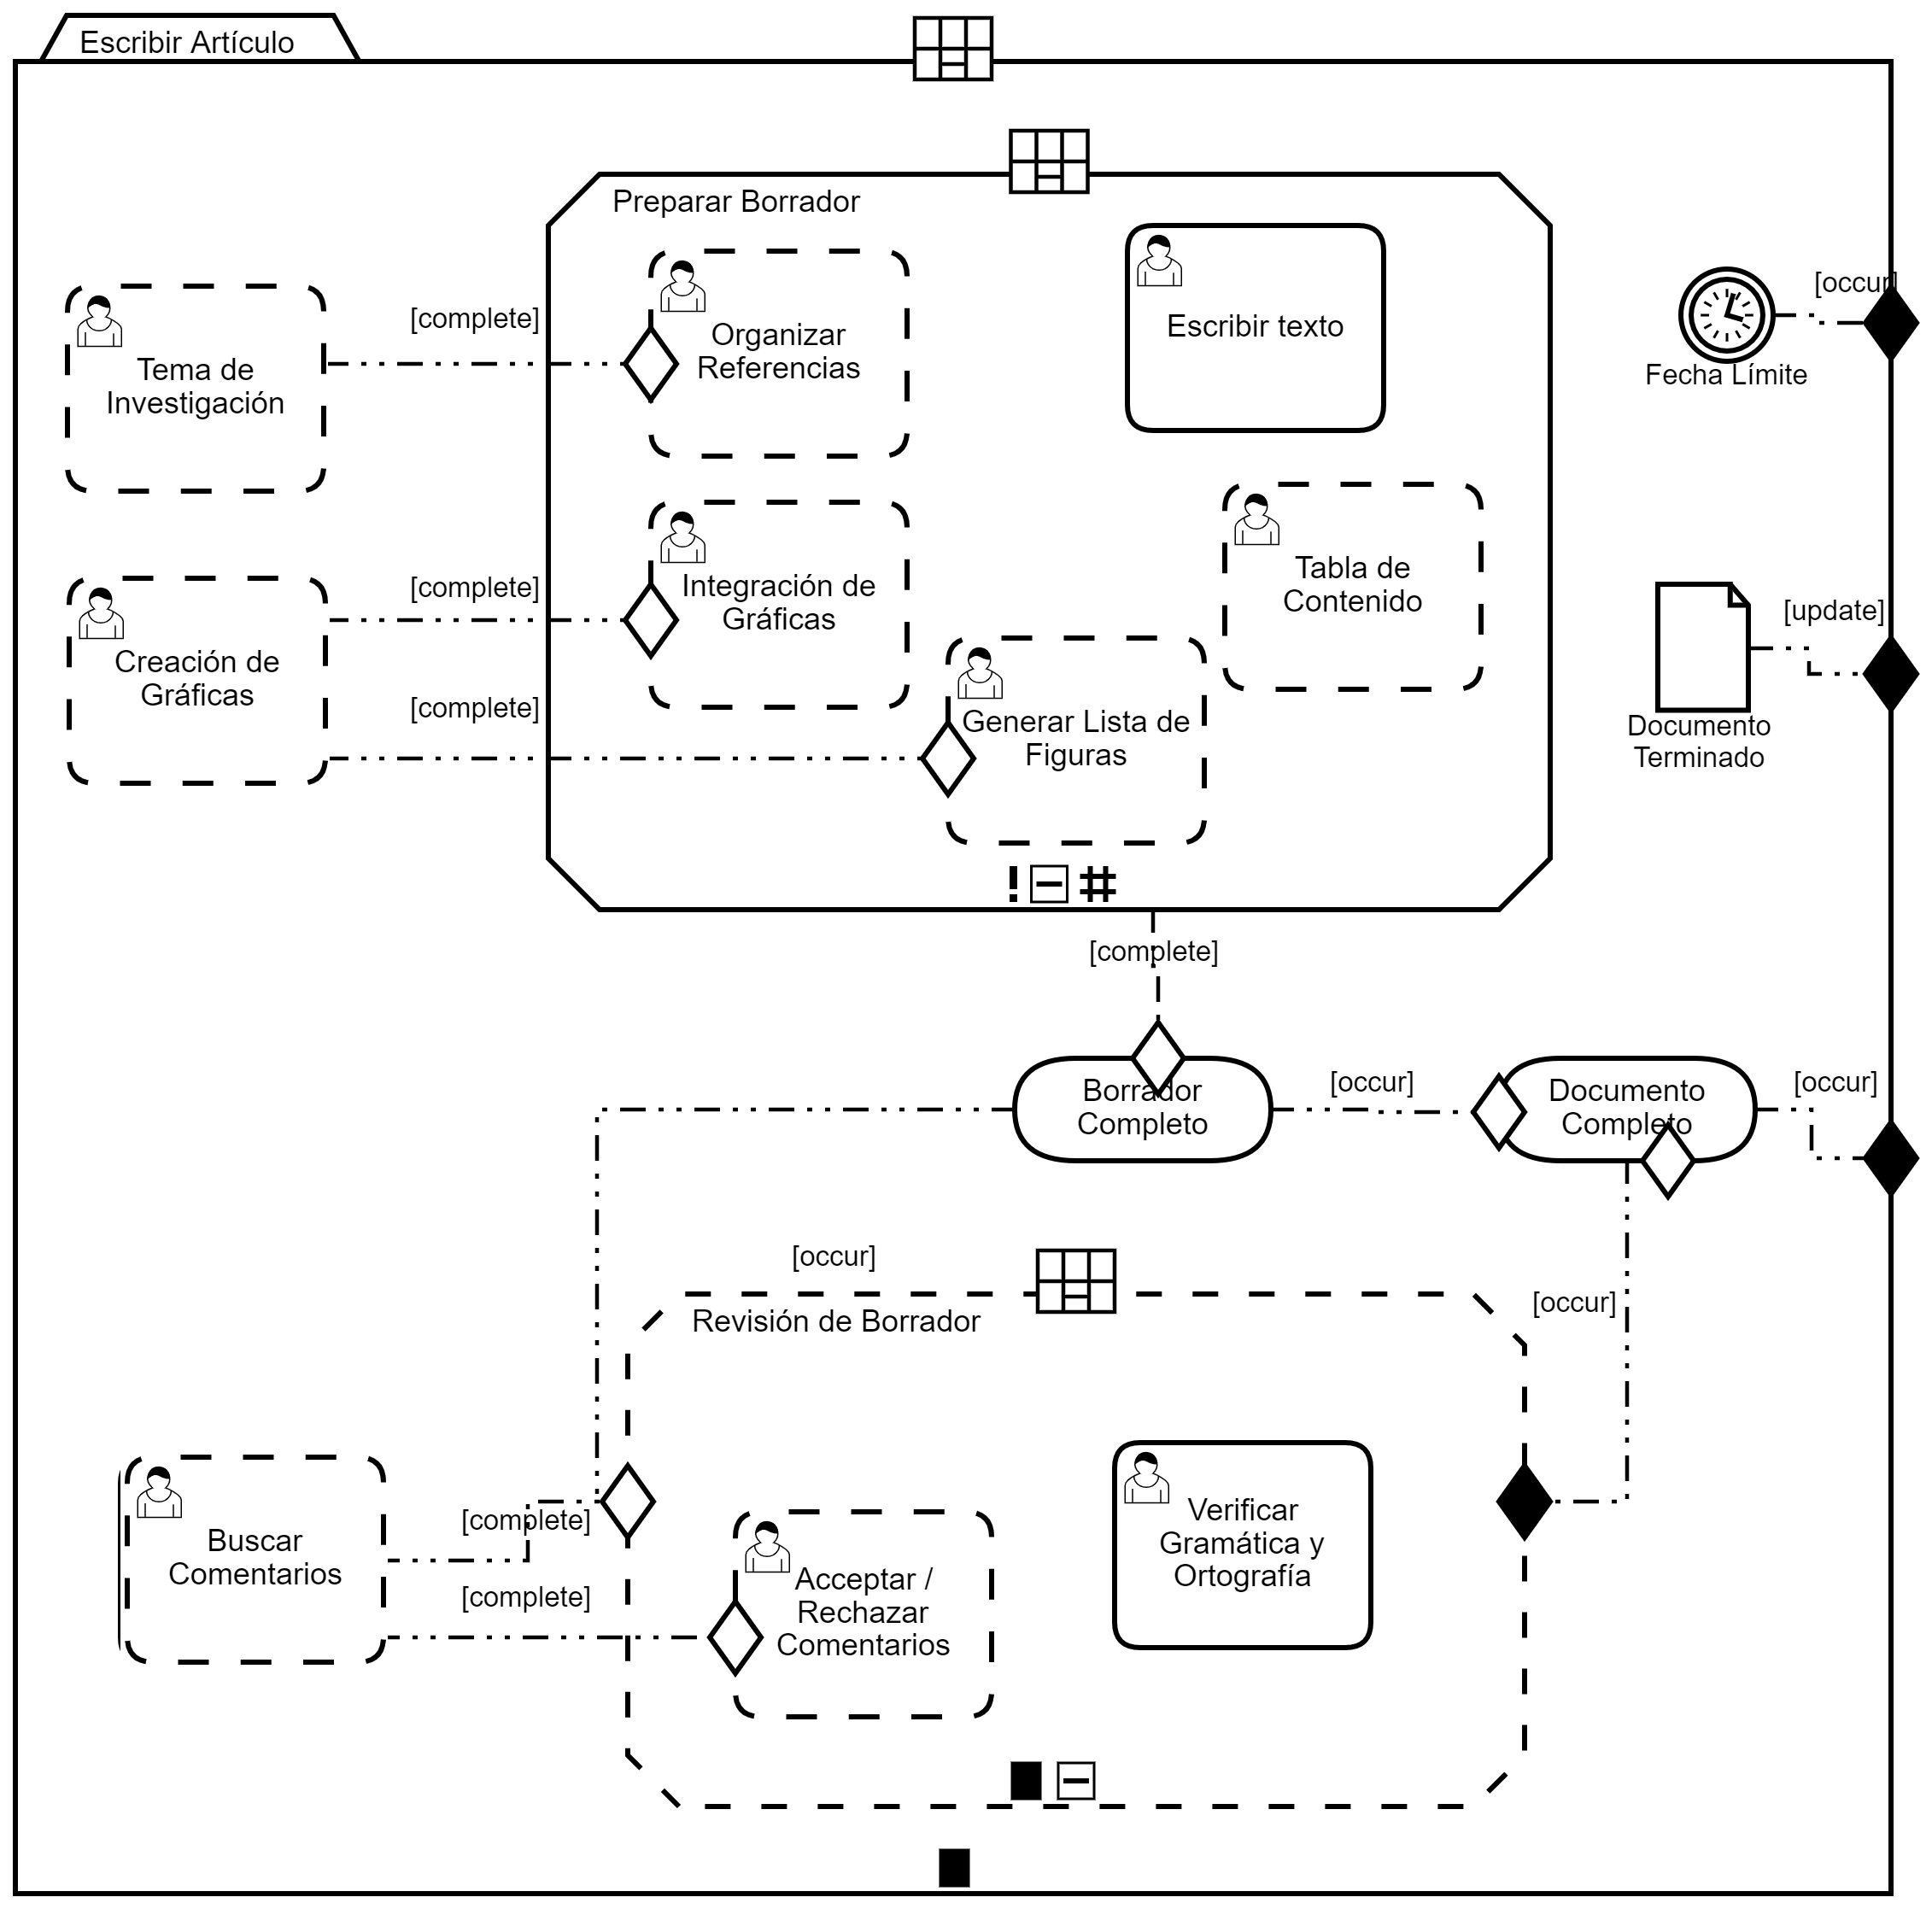
\includegraphics[scale=0.25]{ModeloCMM.png}
  \caption[Modelado de un proceso dinámico]{Modelado de un proceso dinámico con CMMN}
  \label{EjCMMN}
\end{figure}

En \citet{marin2016introduction} se da una aplicación de esta notación a un sistemas de atención de quejas. \citet{breitenmoser2015case} presenta un modelo en notación CMMN para seleccionar candidatos que aplica a un proceso de naturalización en un gobierno local. Tanto en \citet{auer2014business}  como en \citet{omg2011business} se expone una adaptación del ejemplo que se ve n la figura \ref{EjCMMN}, el cual corresponde al proceso de escribir un documento.

%\subsection{Modelo CMMN en un grafo por etapas}

Al hacer la comparación de la notación para el modelado de los procesos estructurados contra la notación de los procesos dinámicos, en el ejemplo que se adaptó de \citet{Cmmn11}, se establece que las líneas punteadas de la figura \ref{EjCMMN} representan la incertidumbre en cuanto a la secuencia que se puede seguir, e incluso a la presencia o no de algunas actividades en la solución a la que se llegue.

%Se vislumbra entonces, cómo esta notación CMMN puede llevarse a un grafo con etapas (como el de la figura \ref{GrafoEtapas}) donde se pueda modelar la incertidumbre en la selección de tareas, disponiendo para cada etapa un conjunto de actividades, de las que no se conoce su probabilidad de ser seleccionada, quedándole al algoritmo de aprendizaje por refuerzo que se implementa para el grafo, el trabajo de recomendar la tarea a seguir después de haber ejecutado alguna tarea de la etapa anterior, restringiendo la selección de una única tarea en cada etapa.

%Para esto se propone que, si dos actividades o tareas b y c están después de una actividad a, pero b y c no son disjuntas, entonces se deben ofrecer b y c en cualquiera de las etapas siguientes, ya que fusionarlas en un nodo ficticio no permite esclarecer con certeza sus prerrequisitos. 

%En este ejercicio, es necesario traer de alguna forma la información pasada, por si alguna actividad que es predecesora de otras se ha ejecutado en etapas anteriores, pero no necesariamente en la inmediatamente anterior. Para ellos es preciso activar una bandera cuando se ejecute una actividad que sea predecesora de otras y condicionar al programa a que revise la bandera, cuando vaya a seleccionar una de las actividades posteriores.

%Un caso específico se presenta en el apéndice \ref{apendicecaso}, el cual se constituye como una parte del trabajo de investigación en el manejo de casos dinámicos de las BPMS que concibió el ingeniero Luis Chaparro, al interior del grupo de investigación GIPROCAS de la Universidad de Boyacá en Colombia.

%Dada esta introducción al caso de estudio, se procede a presentar las consultas bibliográficas correspondientes para establecer si el grafo propuesto ya se encuentra en otra investigación y si ya ha sido abordado un modelo cercano al \textit{L-n-armed-bandits}.

\chapter{Aplicación del método}
\label{Metodo}
El desarrollo de la metodología propuesta en el proyecto es el capítulo central de este documento, aquí se presenta el diseño y la implementación de los algoritmos desarrollados en el proyecto.


%En seguida, se inicia con la presentación de trabajos que dejan ver la importancia que este tipo de propuestas tiene para la comunidad científica internacional.


%\section{DISEÑO DEL PROTOTIPO} 
%Aquí se describe cada uno de los componentes del diseño que compone esta investigación.

\section{Diseño del grafo}

\textit{Inspirados en el grafo del caso de estudio descrito en la sección \ref{Sec:CMMN}, se observó que en la notación de modelado CMMN (ver figura \ref{EjCMMN}) se cuenta con un conjunto de tareas o actividades y de flujos entre ellas, que pueden ser opcionales. Se vio cómo esta situación podía modelarse en un grafo, en el que el problema a solucionar consiste en qué tareas realizar de \textbf{L} etapas consecutivas, para alcanzar al final el objetivo.}

\textit{Un grafo dirigido y conexo permite modelar la estructura de procesos de decisión por etapas de estado y tiempo finitos, como el quw se aprecia en la figura \ref{GrafoEtapas}, cuyos nodos, entre cada dos etapas, tienen las características de un grafo bipartito, es decir que, entre acciones de la misma etapa no deben existir aristas; además, como es conexo, se garantiza que exista al menos una arista que conecte dos etapas sucesivas, así, cada nodo, (excepto los de la última etapa), debe estar conectado al menos con un nodo de la etapa siguiente.}

\begin{figure}[H]
  \centering
    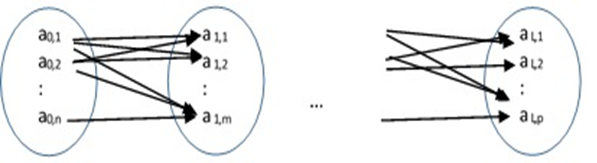
\includegraphics[scale=0.8]{GrafoEtapas.png}
  \caption{Grafo por etapas}
  \label{GrafoEtapas}
\end{figure}

\textit{El grafo es un <<grafo por etapas>>, característica definida en la sección \ref{ConcepGraph}, y el problema que se quiera solucionar debe modelarse como este grafo, con número fijo $L$ de etapas, para que sea susceptible de emplear la aplicación propuesta en esta tesis, por medio de la cual ha de encontrar un camino recomendable para alcanzar un objetivo dado.}

\section{Diseño del modelo matemático}
\label{mat}
Ya se ha dicho que cada uno de los nodos del grafo se constituye en un \textit{ bandit}, pero se desconoce el valor de utilidad que se obtendrá al pasar por cada uno de ellos y solo se conocerá al finalizar la secuencia total de acciones que se decida tomar, es decir, al final de las \textbf{L} etapas.

Además, como la probabilidad total de una ruta determinada, equivale a multiplicar las probabilidades de ir de un nodo a otro hasta culminar la ruta, tal como se hace en un árbol Bayesiano y como se presenta en la fórmula \ref{model1}, al tener el valor de recompensa de haber seleccionado un camino, se decide afectar las probabilidades de pasar entre cada uno de sus nodos, lo que se reflejará en una matriz de probabilidades de transición de estados, donde los estados son los nodos del grafo.
\begin{eqnarray}\label{model1}
P(i_{0} \to i_{1}, ... i_{l-1} \to i_{l}, ... i_{L-1} \to i_{L})=P(i_{0} \to i_{1})P(i_{1} \to i_{2})...P(i_{L-1} \to i_{L}),
\end{eqnarray}
donde $i$ denota el nodo seleccionado en cada una de las etapas, su subíndice $l=0,1,...,L$ denota la etapa a la que pertenece y L denota el número total de etapas. 

Cuando $l = L$ se habrá acumulado una ganancia $G$, que puede ser positiva o negativa. Dado este valor, se hace una modificación a cada una de las probabilidades de transición involucradas y se constituye en el modelo de aprendizaje que se explicará en la sección \ref{aprende}.

\textit{Para el cálculo de estas probabilidades se propone la fórmula \ref{model2}, que, como sucede con la distribución de \textit{SoftMax}, permite generar las probabilidades, las que correspondan a cantidades positivas entre 0 y 1, pero con un fácil cálculo de la sumatoria del denominador, ya que los valores de $A$ corresponden a los ceros y unos de la matriz de adyacencia del grafo.}
\begin{eqnarray}\label{model2}
P(i \to j) = \frac{e^{v_j}}{\sum_k A_{i,k} e^{v_k}},
\end{eqnarray}
donde $A$ es la matriz de adyacencia del grafo y, el valor binario de $A_{i,k}$ permite que solo se tengan en cuenta nodos alcanzables desde el nodo $i$; además, $v$ es el valor de utilidad asociado a cada uno de los nodos del grafo, el cual se va actualizando en cada una de las iteraciones $\tau$ como se muestra en la ecuación \ref{model3}, valor que no necesariamente está relacionado con la recompensa asociada a ese nodo (\textit{bandit}).

\textit{La cantidad del numerador siempre será inferior o, a lo sumo, igual a la cantidad del denominador, dado que el numerador es un término de la sumatoria que aparece en el denominador, la cual está conformada por valores positivos; esto garantiza que los resultados estén en el rango entre 0 y 1; adicionalmente, la suma de todas las probabilidades para los $k$ valores que puede tomar $j$ será 1, lo que corresponde a las probabilidades de transición que se tienen al estar en un nodo $i$;} y, la multiplicación por el valor de cada posición en la matriz de adyacencia $A$, garantiza que únicamente se sumen los exponenciales de nodos adyacentes.

Los valores de utilidad iniciales de los $v$ asociados a cada nodo son cero, de forma que la fórmula \ref{model2} calcula la misma probabilidad para pasar del nodo $i$ a cada uno de sus siguientes, es decir, una probabilidad uniforme; de esta forma se garantiza que la decisión inicial de pasar del nodo $i$ a cualquier otro nodo $j$, es totalmente aleatoria. 

\textit{La probabilidad de transición del nodo i al nodo j va a estar en adelante influenciada por los valores de utilidad $v$ asociados a los nodos, como se explica en la sección \ref{aprende}}.

\section{Diseño del modelo de aprendizaje} 
\label{aprende}

\textit{El modelo busca orientar al agente para que sepa en cada instante cuál es el nodo de la etapa siguiente que a la larga ha de dar el mayor beneficio, lo que se constituye en una particularización de un problema de decisión de Markov donde se hace un muestreo de nodos en cada iteración y se aprovecha la estructura del Grafo por etapas}

Cada uno de los nodos es un \textit{bandit} con un valor de utilidad $v$ asociado; en la etapa inicial se selecciona el nodo origen y en cada etapa siguiente se selecciona un nodo adyacente al ya seleccionado, inicialmente de forma aleatoria porque todas las decisiones inician con probabilidad uniforme, y posteriormente haciendo uso de una matriz de probabilidades de transición de estado, que el autómata irá modificando de acuerdo a su aprendizaje.

Al culminar la secuencia de nodos de las L etapas, se recibe una recompensa que indicará si se ha alcanzado o no el objetivo. De acuerdo a esta recompensa, el valor de utilidad $v$ de cada nodo de la ruta será ponderada para la siguiente iteración sumando un $\delta$, que puede ser positivo o negativo, como se muestra en la fórmula \ref{model3}
\begin{eqnarray}\label{model3}
v_j(\tau + 1) = v_j(\tau) + \delta,
\end{eqnarray}
donde $\delta$ es un parámetro que controla la rata de aprendizaje, ya que $P(i \to j)_{\tau+1} \sim e^{\delta} P(i \to j)_{\tau}$ para pequeños valores de $\delta$.

%El modelo de decisión es lo suficientemente simple como para admitir un tratamiento bayesiano completo de la estimación de parámetros después de cada episodio. Dada la ganancia total $V_L(\tau) = v_1(\tau)+...+v_L(\tau)$, la probabilidad siguiente $P[\vec{v}(\tau) | V_L(\tau)]$ puede escribirse en términos de la ecuaciones (\ref{model1}) y (\ref{model2}).

Luego de varias iteraciones, la matriz de probabilidades tiende a estabilizarse, es decir, sus valores no cambian considerablemente; en ese momento, el modelo ya ha aprendido una ruta específica que reconocerá como la recomendada.

Con los nuevos valores de utilidad $v$ de los nodos se actualizan las probabilidades de selección, de acuerdo a la fórmula \ref{model2}, y los nodos favorecidos por estas probabilidades tendrán un nuevo valor de utilidad $v$ afectado por $\delta$ lo que influirá en los siguientes cálculos de la probabilidades de transición de estados que, finalmente guiará las secuencia de nodos que quedarán en la ruta solución.


\subsection{Exploración}
Este modelo de aprendizaje siempre deja una posibilidad de seleccionar en cada etapa un nodo, que no necesariamente sea el que ha venido dando el mejor resultado, dado que todos los nodos tendrán alguna posibilidad, aunque sea pequeña, de ser elegidos.

Este aspecto se conoce como la exploración, que consiste en dar un margen de duda, por si hay otras opciones que aún no han sido exploradas y que pueden dar una mejor recompensa.

\textit{En las iteraciones iniciales se dará mayor espacio a la exploración, puesto que se inicia con las probabilidades uniformes ya mencionadas y poco a poco se van diferenciando las probabilidades de transición de las opciones que hay desde un nodo $i$. Mientras estas diferencias no sean muy marcadas, se facilitará la exploración de otras decisiones que pueden dar resultados mejores o similares a los ya aprendidos.}

\subsection{Explotación}
La posibilidad de seleccionar con mayor probabilidad los nodos que han estado involucrados en rutas que generan recompensas positivas, permite que el autómata pueda acercarse, cada vez con mayor exactitud, a los valores de los \textit{bandits} que están asociados a cada uno de los nodos de la ruta que él considera que es la más opcionada.

Este aspecto es el que se conoce como explotación que, en términos de juegos de casino, es seguir jugando la misma opción que ha dado los mejores resultados, esperando mejorar aún más.

\textit{En el modelo de aprendizaje propuesto, la explotación tendrá mayor preferencia en las iteraciones finales, donde las probabilidades de transición desde un nodo $i$ ya tienden a tener una acción elegida con una probabilidad cercana a 1 y las demás con probabilidades cercanas a 0. Esta diferencia ya será lo suficientemente grande como para que se siga tomando la misma decisión, de esa iteración en adelante.}


%\section{Selección del camino respuesta}

%\subsection{Modelo Convergencia de la ganancia promedio}
%Luego de que el agente haya generado una matriz de probabilidades de transición entre nodos, y con ella, luego de varias iteraciones, haya encontrado una estabilidad en la ganancia que va calculando, se espera que el argumento que genera esta ganancia sea el camino óptimo a recomendar.

%Por lo tanto, para este modelo lo más importante es la convergencia del valor de la ganancia promedio, lo cual se probará comparándolo con el valor de la ganancia real del mejor camino para un ejemplo con valores conocidos.

%La convergencia de este promedio de ganancias se habrá de notar cuando el camino seleccionado se pruebe un número de veces muy superior a las ocurrencias de otros caminos, predominando el valor de la ganancias del camino elegido.

%\subsection{Modelo Mejor ganancia promedio}
%En este caso, para dar la respuesta se seguirá el modelo tradicional de los \textit{bandit}, donde, luego de elegir  un brazo y de comprobar su recompensa aparente, esta se van acumulando y se van promediando para cada brazo posible de ser seleccionado, para luego de varias búsquedas, escoger el brazo cuya ganancia promedio sea la mejor, como se ve en la ecuación \ref{Gprom}, ya presentada en la fundamentación teórica.
%\begin{eqnarray}\label{Gprom}
%Q_t(a) = \frac{R_1+R_2+ ...+R_{Nt(a)}}{N_t(a)}
%\end{eqnarray}
%donde los R son las recompensas (positivas o negativas) que se perciben al explorar cada opción y N es el número de veces que esa opción se ha explorado.

%El argumento de esta función, para el modelo propuesto, será la secuencia de $L$ nodos que representan cada ruta. Se tomará el mayor valor de $Q$ y su argumento se dará como camino óptimo a recomendar.

%Aquí se tendrá que asociar a cada secuencia de nodos, que eventualmente sea conformada, un contador y un valor medio de las ganancias que va acumulando durante la ejecución del programa, para poder, de ellas seleccionar la mejor para dar la respuesta.

\section{Construcción del algoritmo}
\label{algoritmos}
El desarrollo y ejecución de los algoritmos se hizo en el lenguaje de programación
Python 3.7, en un computador personal con procesador Intel Core i3-6006U de 2.00 GHz con 4.0 GB de memoria RAM, con sistema operativo Windows 10, de 64 bits.

Para la pruebas finales se migró la aplicación a un computador de la Universidad de Boyacá con procesador Intel(R) Xeon(R) Core i3-6006U de 3.50 GHz con 16.0 GB de memoria RAM, con sistema operativo Windows 10 Pro, de 64 bits.

Para los cálculos de los algoritmos se utilizaron en Python las librerías numpy, operator y math, y para la visualización de las simulaciones se empleó la librería matplotlib.

Para simular un problema de aplicación, donde se conocen la cantidad de etapas y la cantidad de tareas posibles para cada etapa, se diseña e implementa un algoritmo que recibe estos parámetros de entrada y genera aleatoriamente una matriz de adyacencia con estos datos y los valores de los \textit{bandits} asociados a cada uno de los nodos. Se verifica que el número y disposición de las aristas sean tales que cada nodo se conecte con al menos uno de la etapa siguiente. 
La cantidad de aristas que se generen entre etapas es un parámetro que se tiene en cuenta para la generación aleatoria del grafo, el cual corresponde a la densidad del grafo.

Cada uno de los nodos del grafo, eventualmente, representa una actividad a desarrollar dentro de una ruta de actividades que debe contener exactamente un nodo de cada etapa del grafo. A cada uno de esos nodos se le ha asociado un \textit{bandit}, que no es otra cosa que un número que indica la recompensa que se obtiene al jugar este \textit{bandit} en un casino, cantidad que para el caso de la simulación será positiva o negativa; y alrededor de la cual se generan los valores distorsionada que el jugador realmente recibe al seleccionar ese \textit{bandit} en el casino (que casi nunca será el valor real).

Cada \textit{bandit} se genera con una distribución normal con media en cero y desviación estándar de uno, pero podrá adecuarse su magnitud, si es conveniente, tanto para el manejo computacional, como para la simulación de un ejemplo real; los valores que se obtienen se consideran los valores reales y, son los que debe descubrir el algoritmo. Este valor real será la base para la generación de los valores distorsionados de los \textit{bandits} en cada una de las épocas o iteraciones, los cuales se generan tomando su valor inicial o real como media de otra distribución normal, también con desviación estándar de 1.

En cada iteración se calcula una ganancia real, con los valores reales que se generaron para cada uno de los nodos por donde pase la ruta seleccionada por el algoritmo. También se calcula, para cada iteración la ganancia con los valores distorsionados de la misma ruta, para efectos de poder compararlas eventualmente. Con esta última ganancia se hacen los cálculos de probabilidades de selección de nodos.

%, con los cuales se calcula la ganancia al final de la ruta, con la que se simula el éxito o el fracaso, de acuerdo al signo de la misma. 

En seguida se presentan las versiones de pseudocódigo que se fueron implementando y probando, las cuales se complementan para dar la propuesta final.

\subsection{Generador de bandits}

Se inicia con la creación y prueba de la selección del \textit{bandit} que mejor probabilidad tenga asociada. El algoritmo aplica la fórmula del  promedio de las recompensas sobre el número de veces que fue seleccionado \ref{Q}.

Como se aprecia en el pseudocódigo \ref{Bandit} se generó para cada  uno una media con distribución Normal (0,1) y a partir de cada valor se generaron otros valores distorsionados, adicionando un ruido, también generado por distribución Normal (0,1). Este código se probó varias veces y siempre encontró la acción $a$ asociada al \textit{bandit} con mejor probabilidad.



\begin{algorithm} [h]
\caption{Genera-bandit(T=Iteraciones, n=Número de acciones,
$\epsilon$=$\epsilon$-greedy)} 
\label{Bandit}
\begin{algorithmic}[1]
\FOR{t = 1 \TO T}
     \STATE r = np.random.sample()
     \IF{$r > \epsilon$}
        \STATE  a = np.argmax(Q)
     \ELSE
        \STATE a = np.random.randint(0,n)
     \ENDIF
     \STATE sQ[a] = sQ[a] + q[a] + np.random.randn()
     \STATE Nt[a] =  Nt[a] + 1
     \STATE Q[a] = sQ[a] / Nt[a]
     \STATE Imprima('a ',a)
\ENDFOR
\end{algorithmic}
\end{algorithm}

La figura \ref{AlgBandit} es el resultado gráfico de una corrida de este algoritmo con 400 iteraciones, 10 acciones y $\epsilon$=0.3. La línea roja representa la recompensa promedio que va encontrando en cada iteración y la línea horizontal que está ubicada en 1 representa el número del \textit{bandit} que en promedio obtiene la mejor ganancia al finalizar las iteraciones, respuesta que corresponde exactamente con los valores asignados inicialmente.

\begin{figure} [H]
    \label{Resul2}
	\centering
	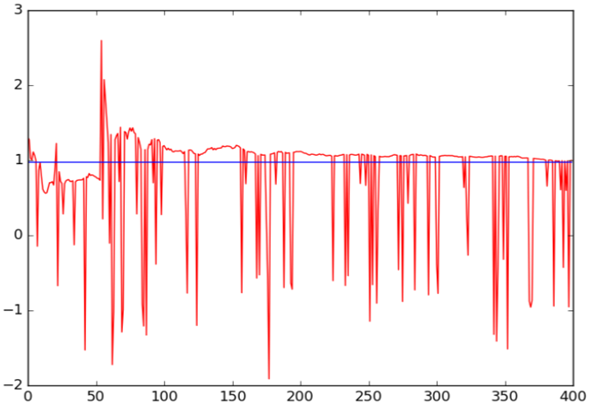
\includegraphics[scale=0.6]{AlgBandit}
	\caption[Resultado de la selección de brazo usando \textit{bandits}]{Selección de la mejor acción usando el algoritmo de los \textit{bandits}}
	\label{AlgBandit}
\end{figure}

La oscilación de la línea roja se produce por la exploración que el algoritmo hace de otras alternativas diferentes a la que en cada momento parece ser la mejor. No se esperan los mismos valores cada vez que se esté probando el mismo \textit{bandit}, porque los valores que recibe son los que fueron distorsionados con el ruido. 

\subsection{Generador de la matriz de adyacencia}

Posteriormente se implementó un código que genera aleatoriamente matrices de adyacencia del grafo por etapas. Estas matrices deben ser escalonadas, deben obedecer a los requisitos de precedencia de nodos entre etapas y deben tener al menos un 1 en cada fila para garantizar la conexión de las etapas. El pseudocódigo \ref{Matriz} corresponde a tales características.

Este algoritmo recibe los datos de número de etapas y número de nodos por cada etapa que ya han de estar definidos con anterioridad.

\begin{algorithm} [h]
\caption{Genera-matriz(L=Cantidad de etapas, M[L]=Nodos por etapa} 
\label{Matriz}
\begin{algorithmic}[1]
\STATE Calculate: n=Cantidad de nodos
\STATE Generate: Ad[nxn] = zeros
\STATE nodoi=0
\STATE nodofin= nodoi+M[0]-1
\FOR{l = 1 \TO L-1}
    \FOR{i in range(nodoi, nodofin+1)}
        \STATE nodohi=nodofin+1
        \STATE nodohfin= nodohi+M[l+1]-1
        \STATE sumafila=0
        \FOR{j in range(nodohi, nodohfin+1)}
            \STATE arg = np.random.randint(2, size=1)
            \STATE A[i,j] = arg 
            \STATE sumafila += A[i,j]
            \IF{umafila == 0}
                \STATE  A[i,j] = 1
            \ENDIF
        \ENDFOR
    \ENDFOR
    \STATE nodoi=nodohi
    \STATE nodofin=nodohfin
\ENDFOR     
\STATE Imprima('A ',A)
\end{algorithmic}
\end{algorithm}

Este código también se probó varias veces y siempre arrojó resultados adecuados de matrices escalonadas, adecuadas para el grafo por etapas diseñado, como el ejemplo que se muestra en la figura \ref{MatrizAy}. 

\begin{figure} [H]
    \label{Resul2}
	\centering
	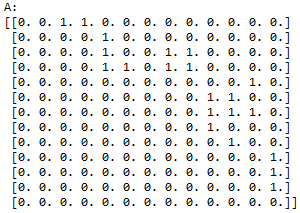
\includegraphics[scale=0.8]{MatrizAy}
	\caption{Resultado de la matriz de adyacencia para un grafo por etapas}
	\label{MatrizAy}
\end{figure}

\subsubsection{Generación de una ruta aleatoria}

Se implementó la fusión del algoritmo para la generación de la matriz de adyacencia, con el que genera los valores asociados a cada nodo o \textit{bandit}; el pseudocódigo correspondiente se probó con valores aleatorios, obteniendo siempre la matriz escalonada que se esperaba y los valores asociados a los \textit{bandits}.

Se le adicionó una funcionalidad para que tomara una ruta factible, teniendo en cuenta la matriz de adyacencia para encontrar los vecinos de cada nodo, la cual se presenta en el algoritmo \ref{Ruta}. Las pruebas que se hicieron funcionaron siempre correctamente.

\begin{algorithm} [h]
\caption{Genera-rutas(L=Cantidad de etapas, A=Matriz de adyacencia} 
\label{Ruta}
\begin{algorithmic}[1]
\STATE n[0]=0
\FOR{l = 1 \TO L}
    \STATE nzv = np.nonzero(A[o, ])
    \STATE nzv = np.reshape(nzv,-1) :vector de nodos adyacentes
    \FOR{i in range(o, len(nzv)}
        \STATE d = np.random.choice(nzv, 1)
        \STATE R[l]=d
    \ENDFOR   
\ENDFOR
\STATE Imprima('Ruta ',R)
\end{algorithmic}
\end{algorithm}

\textit{Los valores que se asignaron aleatoriamente a los \textit{bandits} sirven para calcular una ganancia total por cada ruta que contenga nodos de las $L$ etapas; esta ganancia equivaldría a la \textit{ganancia real} que se obtendría si se supieran los valores de utilidad asociados a cada \textit{bandit}. Así mismo, en cada iteración que ejecute el código, el autómata recibirá una información distorsionada del valor de cada \textit{bandit}, de acuerdo a la distribución Normal que ya se ha explicado; con estos valores el autómata ha de calcular la ganancia que realmente estará recibiendo al final de las $L$ etapas, a la que en adelante se reconocerá como \textit{ganancia distorsionada}. }

El cálculo de la ganancia distorsionada se muestran en los algoritmos siguientes como $Gain_{path}$, la cual va recogiendo en cada etapa la ganancia del nodo seleccionado $Gan_{orig}$, de acuerdo a los valores de utilidad de los \textit{bandit}, que realmente recibe el autómata y que se generan en cada iteración como $Gan_{n}$.

\subsection{Encontrando la ruta óptima}

\textit{Aquí se presentan dos momentos diferentes: Inicialmente aquel donde la escogencia del siguiente nodo de un camino, solo tiene que estar dentro del conjunto de vecinos del nodo actual, pero todos con la misma probabilidad de ser seleccionados; este modelo se reconocerá como Probabilidades Uniformes. Seguidamente se implementa la generación de la matriz de probabilidades de transición de pasar de un nodo a otro, la cual se basa en un fundamento matemático específico que se presentó en la sección \ref{mat}, modelo que se espera que converja a una única respuesta con la mejor ruta encontrada; y este se reconocerá como Probabilidad Modelada.}

\subsection{Búsqueda con probabilidad uniforme}

Inicialmente los nodos de una etapa que sean adyacentes al nodo que ha sido seleccionado en la etapa anterior, tienen una probabilidad uniforme de que sean seleccionados. Este algoritmo se construye básicamente, incluyendo un contador de iteraciones para que el algoritmo de generación de rutas factibles se ejecute una cantidad dada de veces determinada y una selección de la ruta que al final de las iteraciones hubiera obtenido la ganancia promedio, para entregarla como respuesta. 

El pseudocódigo queda como se ve en el cuadro del algoritmo \ref{PsUniforme}, que con los datos de entrada y los generados aleatoriamente para el grafo, calcula una ruta de nodos de cada etapa, solamente teniendo en cuenta que el siguiente nodo forme parte de los vecinos del presente.

\begin{algorithm} [h]
\caption{L-n-bandit-Uniforme(L=Cantidad de etapas, M[L]=Nodos por etapa,
n=Cantidad de nodos)} \label{PsUniforme}
\begin{algorithmic}[1]
\STATE Generate: Ad[nxn] = Matriz de adyacencia
\STATE Generate: B[n] = Bandits reales
\FOR{t = 1 \TO T}
    \STATE Generate: $Gan_{n}$
    \STATE $Gain_{path}$ = 0
    \STATE Initialize: orig = 0
    \STATE Add: orig in path
    \FOR{l = 1 \TO L-1}
        \STATE Generate: $nvz_{orig}$ = vecinos de orig
        \STATE Random: ${dest \in nvz_{orig}}$
        \STATE $orig = dest$
        \STATE Add: orig in path
        \STATE $Gain_{path}$ =+ $Gan_{orig}$
     \ENDFOR
     \STATE Imprima: path
\ENDFOR
\end{algorithmic}
\end{algorithm}

\subsection{Búsqueda con probabilidades aprendidas}
Posteriormente se implementó el cálculo de la matriz de probabilidades de transición con las fórmulas explicadas en la sección \ref{mat} cuyo pseudocódigo se muestra en el cuadro algorítmico \ref{Pseudo}. A diferencia del anterior, la selección del nodo siguiente al presente en cada ruta, no solo va a tener en cuenta la vecindad con este último, sino la probabilidad de transición a cada nodo vecino, consignada en la matriz de probabilidad de transición que aquí se genera y se actualiza, de acuerdo a las ganancias que reciba el camino, en cada iteración, como se explica en seguida.

\begin{algorithm} [h]
\caption{L-n-bandit(L=Cantidad de etapas, M[L]=Nodos por etapa )
} 
\label{Pseudo}
\begin{algorithmic}[1]
\STATE Calculate: n=Cantidad de nodos
\STATE Initialize: v[n] = 0
\STATE Generate: Ad[nxn] = Matriz de adyacencia
\STATE Generate: B[n] = Bandits reales
\FOR{t = 1 \TO T}
     \STATE Initialize: orig = 0
     \STATE Add: orig in path
     \STATE $P(i \to j) = \frac{e^{v_j}}{\sum_k A_{i,k} e^{v_k}},$
     \STATE Generate: $Gan_{n}$
     \STATE $Gain_{path}$ = 0
     \FOR{l = 1 \TO L-1}
        \STATE Generate: $nvz_{orig}$ = vecinos de orig
        \STATE Select: $dest \in nvz_{orig}$  by $P(i \to j)$
        \STATE $orig = dest$
        \STATE Add: orig in path
        \STATE $Gain_{path}$ =+ $Gan_{orig}$
     \ENDFOR
     \IF{$Gain_{path} > 0$}
        \STATE v[n+1] = v[n] + $\delta$ by i $\in$ path
     \ELSE
        \STATE v[n+1] = v[n] - $\delta$ by i $\in$ path   
     \ENDIF   
     \STATE Imprima: path
\ENDFOR
\end{algorithmic}
\end{algorithm}

Para la primera iteración se maneja una probabilidad uniforme y para las demás iteraciones, se calculan las probabilidades de transición entre nodos. En cada iteración se selecciona un nodo de la etapa inicial, se calculan sus vecinos o nodos alcanzables y se selecciona el que mayor probabilidad de transición presente, para guardarlo en la ruta y proceder a hacer la búsqueda de sus vecinos en la siguiente etapa, hasta llegar a la última, usando siempre el mismo criterio de selección.

Una vez se conozca la ganancia o pérdida al final de la iteración, se actualizan los valores de utilidad $v$ de cada nodo de esa ruta, de acuerdo a la fórmula \ref{model3}, este valor se utiliza para calcular las nuevas probabilidades de transición con la fórmula \ref{model2}, que se tendrán en cuenta en la siguiente iteración. Cabe anotar que al final de cada etapa solo se afectan las probabilidades de transición de los nodos involucrados en la ruta seleccionada, pero que al iniciar cada iteración se cuenta con todas las modificaciones que hayan sufrido estas probabilidades en las iteraciones anteriores de esta simulación.

Se recuerda que la selección del siguiente vecino está fuertemente influenciada por las probabilidades de transición, constituyéndose en la explotación de los caminos preferidos, pero siempre deja un porcentaje de posibilidad de escoger cualquier nodo que no sea el de mayor probabilidad de transición asociada, lo que permite resolver el problema de la exploración, propio de la teoría de los \textit{bandits}, que garantiza la búsqueda de mejores soluciones que no se han considerado aún.

Al final de las iteraciones definidas, el simulador debe converger a la mejor ruta que haya estudiado, que puede ser la óptima, como se verá en la siguiente sección.

\section{Pruebas}

\subsection{Grafo para las pruebas}

Aunque el algoritmo se ha diseñado para generar grafos aleatorios, se hace necesario generar uno particular para poder comparar los valores resultantes de las ejecuciones del algoritmo con este. Tal grafo debe ser de un tamaño adecuado para poder calcular todas las posibles rutas desde un nodo inicial hasta uno final con sus respectivas ganancias; además, los nodos deberán tener asociados valores de ganancias, de forma que se pueda establecer claramente cuál es la ruta óptima.

\begin{figure}[h]
  \centering
    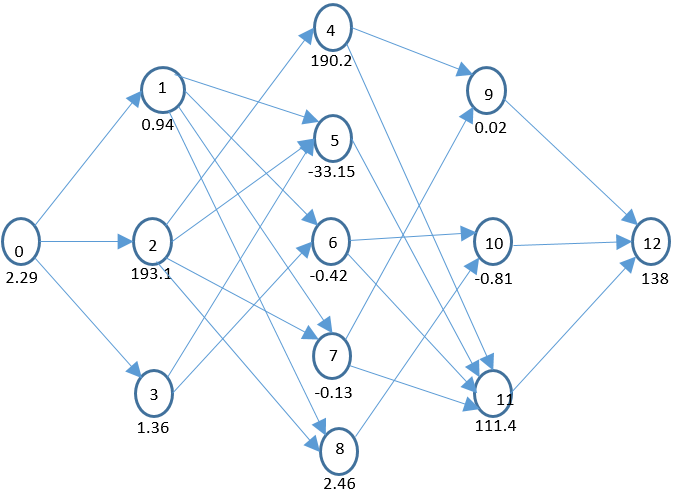
\includegraphics[scale=0.5]{Grafo5L.png}
  \caption[Grafo Modelo]{Grafo Modelo con 5 etapas y 13 nodos}
  \label{Grafomodelo}
\end{figure}

Se realizan estas pruebas entonces, con un grafo de 5 etapas y 13 nodos, dispuestos como se ve en la figura \ref{Grafomodelo}, inicialmente con matriz de adyacencia aleatoria, así como los valores de utilidad de sus \textit{bandits}, pero obligando a que uno de ellos por etapa tenga un mayor valor que los demás, para identificar con facilidad la mejor ruta y así verificar su funcionamiento.


\subsection{Pruebas con probabilidad uniforme}

El algoritmo cuyo pseudocódigo se presentó en el cuadro \ref{PsUniforme}, se ejecutó con 99 intervalos de tiempo. La figura \ref{fig:uniforme} muestra uno de los resultados. 

\begin{figure}[H]
	\centering
	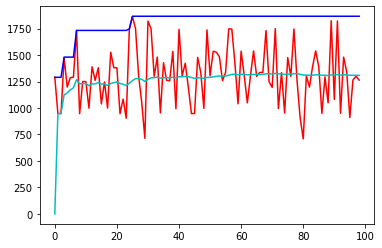
\includegraphics[scale=1]{Uniforme}
	\caption{Resultado con probabilidad uniforme}
	\label{fig:uniforme}
\end{figure}

En esta gráfica, la curva superior azul corresponde a la ganancia real de la mejor ruta probada hasta el momento, calculada con el valor de utilidad asignado a los \textit{bandits}; en la curva roja, la más inestable, se presentan las ganancias distorsionadas obtenidas en cada instante de tiempo por la ruta seleccionada, calculada con los valores distorsionados con ruido para los \textit{bandits}; y en la curva inferior verdosa se muestra el promedio acumulado de estas ganancias, el cual converge a un único valor a través del tiempo, pero no trata de acercarse al valor real.

\subsection{Pruebas con probabilidades aprendidas}

Con 33 iteraciones (T=33) el algoritmo \ref{Pseudo} generó la gráfica de la figura \ref{Resul2}, en la cual se pueden apreciar los valores que van tomado su ganancia y su ganancia promedio, la cual convergió rápidamente hacia el valor de la mejor ganancia real. La mejor ganancia real se calculó para la mejor ruta que el mismo algoritmo haya encontrado: esto permite que el software sea el que estime dicha ruta y su ganancia, sin una intervención manual.

\begin{figure} [H]
	\centering
	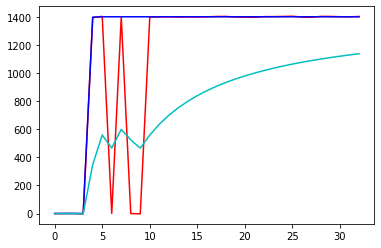
\includegraphics[scale=1]{Resul2}
	\caption{Resultado con probabilidad aprendida}
	\label{Resul2}
\end{figure}
En esta gráfica, al igual que en la del modelo anterior, la curva superior azul corresponde a la ganancia de la mejor ruta probada hasta el momento, calculada con el valor de utilidad real asignado a cada uno de los \textit{bandits}; en la curva más inestable se presentan las ganancias distorcionads obtenidas en cada instante de tiempo por la ruta seleccionada; y en la curva inferior verdosa se muestra el promedio acumulado de estas ganancias, el cual, trata de acercarse a la curva de la ganancia real. 

De otra parte, para estimar el comportamiento del algoritmo se dejan fijos en el grafo los datos de la matriz de adyacencia y del vector de valores de utilidad reales de los \textit{bandits}, para ejecutar los experimentos que se explican en el siguiente capítulo.


%y se estima una ganancia que se genera aleatoriamente a una desviación estándar de su \textit{bandit} ... La decisión de usar una generación de números aleatorios que siguen una distribución normal con media en cero y desviación estándar en 1, es porque es la utilizada en la literatura de aprendizaje por refuerzo \citep{sutton1992reinforcement}, con la cual se ha probado el funcionamiento del modelo de decisión \textit{n-armed bandit}. 
%\chapter{Resultados obtenidos}
\label{resul}

\section{Construcción del algoritmo}
El algoritmo diseñado e implementado recibe como parámetros de entrada la cantidad de etapas y la cantidad de nodos de cada una de ellas; además, genera aleatoriamente una matriz de adyacencia con estos datos, luego de calcular el número de nodos, para los cuales también genera aleatoriamente los valores de los \textit{bandits} asociados. Así, la cantidad de etapas y de nodos de cada etapa, serán los valores que el simulador tendrá en cuenta para generar el grafo, verificando que el grupo de aristas sea suficiente para que cada nodo se conecte con al menos uno de la etapa siguiente, así como cumpliendo las demás restricciones de grafo propuesto. 

Cada uno de los nodos del grafo, eventualmente, representa una actividad a desarrollar dentro de una ruta de actividades que debe contener exactamente un nodo de cada etapa del grafo. A cada uno de esos nodos se le ha asociado un \textit{bandit}, que no es otra cosa que un número que indica la recompensa que se obtiene al jugar este \textit{bandit} en un casino, cantidad que para el caso de la simulación será positiva o negativa, pero con magnitud menor a 1; y alrededor de la cual se generan los valores distorsionada que el jugador realmente recibe al seleccionar ese \textit{bandit} en el casino (que casi nunca será el valor real).

Cada \textit{bandit} se genera con una distribución normal con media en cero y desviación estándar de uno; los valores que se generen se consideran los valores reales que debe descubrir el algoritmo. Este valor real será la base para la generación de los valores distorsionados en cada una de las etapas, los cuales se generan tomando ese valor inicial o real como media de otra distribución normal, también con desviación estándar de 1.

En cada algoritmo se calcula una ganancia real, para cada iteración, con los valores reales que se generaron y que corresponden a cada uno de los nodos por donde pase la ruta seleccionada por el algoritmo. También se calcula, para cada iteración la ganancia con los valores distorsionados de la misma ruta, para efectos de poder compararlas eventualmente. Con esta última ganancia es que se harán los cálculos de probabilidades de selección de nodos en las últimas propuestas.

%, con los cuales se calcula la ganancia al final de la ruta, con la que se simula el éxito o el fracaso, de acuerdo al signo de la misma. 

En seguida se presentan las versiones de pseudocódigo que se fueron implementando y probando, las cuales se comparan en su desempeño para dar la mejor como propuesta final.

\subsection{Con probabilidad uniforme}
Inicialmente los nodos de una etapa que sean adyacentes al nodo que ha sido seleccionado en la etapa anterior, tienen una probabilidad uniforme de que seleccionados. 

El pseudocódigo queda como se ve en el cuadro del algoritmo \ref{PsUniforme}, que con los datos de entrada y los generados aleatoriamente para el grafo, calcula una ruta de nodos de cada etapa, solamente teniendo en cuenta que el siguiente forme parte de los vecinos del presente.

\begin{algorithm} [h]
\caption{L-n-bandit-Uniforme(L=Cantidad de etapas, M[L]=Nodos por etapa, n=Cantidad de nodos)} \label{PsUniforme}
\begin{algorithmic}[1]
\STATE Generate: Ad[nxn] = Matriz de adyacencia
\STATE Generate: B[n] = Bandits reales
\FOR{t = 1 \TO T}
     \STATE Initialize: orig = 0
     \STATE Add: orig in path
     \FOR{l = 1 \TO L-1}
        \STATE Generate: $nvz_{orig}$ = vecinos de orig
        \STATE Random: ${dest \in nvz_{orig}}$
        \STATE $orig = dest$
        \STATE Add: orig in path
     \ENDFOR
     \STATE Calculate: $Gan_{path}$
\ENDFOR
\end{algorithmic}
\end{algorithm}

%\begin{figure}
%	\centering
%	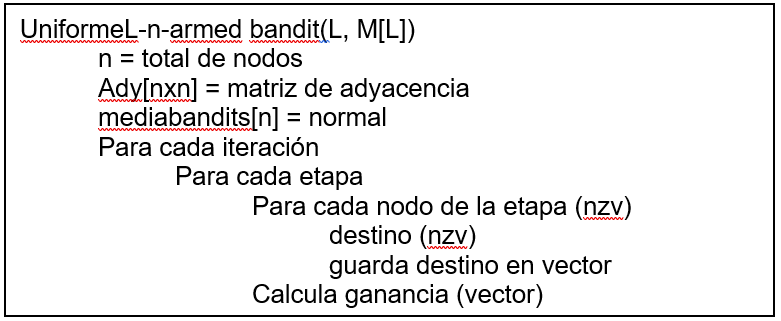
\includegraphics[scale=0.5]{Psuniforme}
%	\caption{Pseudocódigo L-n-armed bandit con Probabilidades Uniformes}
%	\label{PsUniforme}
%\end{figure}

\subsection{Con probabilidades aprendidas}
Posteriormente se implementó el cálculo de la matriz de probabilidades de transición con las fórmulas explicadas en la sección \ref{mat} cuyo pseudocódigo se muestra en el cuadro algorítmico \ref{Pseudo}. A diferencia del anterior, la selección del nodo siguiente al presente en cada ruta, no solo va a tener en cuenta la vecindad con este último, sino el valor que el nodo a seleccionar tenga asociado en la matriz de probabilidad de transición que aquí se genera y se actualiza, de acuerdo a las ganancias que reciba el camino, en cada iteración, como se explica en seguida.

\begin{algorithm}
\caption{L-n-bandit(L=Cantidad de etapas, M[L]=Nodos por etapa, n=Cantidad de nodos)} 
\label{Pseudo}
\begin{algorithmic}[1]
\STATE Initialize: w[n] = 0
\STATE Generate: Ad[nxn] = Matriz de adyacencia
\STATE Generate: B[n] = Bandits reales
\FOR{t = 1 \TO T}
     \STATE Initialize: orig = 0
     \STATE Add: orig in path
     \STATE $P(i \to j) = \frac{e^{v_j}}{\sum_k A_{i,k} e^{v_k}},$
     \FOR{l = 1 \TO L-1}
        \STATE Generate: $nvz_{orig}$ = vecinos de orig
        \STATE Select: ${dest \in nvz_{orig} by P(i \to j)}$
        \STATE $orig = dest$
        \STATE Add: orig in path
     \ENDFOR
     \STATE Calculate: $Gan_{path}$
     \IF{$Gan_{path} > 0$}
        \STATE w[n] = w[n] + $\delta$ by i $\in$ path
     \ENDIF    
\ENDFOR
\end{algorithmic}
\end{algorithm}

Para la primera iteración se maneja una probabilidad uniforme. Para las demás iteraciones, calcula las probabilidades de transición entre nodos y en cada etapa recorre los nodos de una etapa desde la inicial, hasta la penúltima y para cada nodo encuentra sus vecinos o nodos alcanzables, selecciona el que mayor probabilidad de transición presente, o uno al azar cuando aún no estén estipuladas esas probabilidades, para guardarlo en la ruta y proceder a hacer la búsqueda de sus vecinos en la siguiente etapa, con el mismo criterio de selección explicado.

Una vez se conozca la ganancia o pérdida al final de la iteración, se actualizan los valores de preferencia de cada nodo de esa ruta, de acuerdo a la fórmula \ref{model3}, este valor se utiliza para calcular las nuevas probabilidades de transición con la fórmula \ref{model2}, que se tendrán en cuenta en la siguiente iteración. Cabe anotar que al final de cada etapa solo se afectan las probabilidades de transición de los nodos involucrados en la ruta seleccionada, pero que al iniciar cada iteración se cuenta con todas las modificaciones que hayan sufrido estas probabilidades en las iteraciones pasadas de la simulación.

La selección del siguiente vecino está fuertemente influenciada por las probabilidades de transición, constituyéndose en la explotación de los caminos preferidos, pero siempre deja un porcentaje de posibilidad de escoger cualquier nodo que no sea el de mayor probabilidad de transición asociada, lo que permite resolver el problema de la exploración, propio de la teoría de los \textit{bandits}, que garantiza la búsqueda de mejores soluciones que no se han considerado aún.

%Al final de las iteraciones definidas, el simulador converge a la mejor ruta que haya estudiado, que puede ser la óptima. En forma gráfica se puede apreciar esta convergencia en la ganancia que se recibe que al final de las iteraciones tiende a ser una constante. 

%\begin{figure}\label{Pseudo}
%	\centering
%	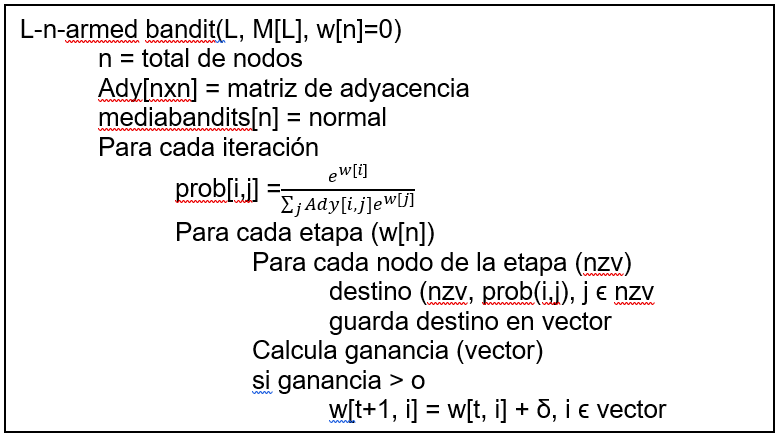
\includegraphics[scale=0.5]{Pseudo}
%	\caption{Pseudocódigo L-n-armed bandit }
%\end{figure}

%El algoritmo recibe los valores de L (número de etapas), M (vector con el número de nodos de cada etapa) y el vector w (valores de preferencia de cada nodo) inicializado en ceros. Calcula n que es la cantidad total de nodos, genera aleatoriamente la matriz de adyacencia y los \textit{bandit} para cada nodo.

%Con los datos de los nodos seleccionados se calcula la ganancia al final de las L etapas de acuerdo a esta se actualizan los valores de preferencia de cada nodo (w) con los que se calcular nuevamente las probabilidades de transición hacia sus vecinos para una nueva iteración.

%\section{PSEUDOCÓDIGO Y PRUEBAS}

%Inicialmente se toma un grafo modelo que se presenta en la figura \ref{Grafomodelo} con su matriz de adyacencia y valores de sus \textit{bandits} fijos. Se le da libertad a los algoritmos a evaluar, que decidan las rutas a seguir de forma aleatoria.

%\begin{figure}[H]
%\label{Grafomodelo}
%	\centering
%	\includegraphics[scale=0.5]{Grafomodelo}
%	\caption{Grafo de 5 etapas con 13 nodos}
%	\label{Pseudocódigo}
%\end{figure}

%El desempeño del algoritmo propuesto se compara con un algoritmo que asigna probabilidades uniformes a las transiciones entre un nodo y sus vecinos, quedando la decisión del nodo a seguir al azar. El pseudocódigo correspondiente se ve en el cuadro \ref{PsUniforme}. Como era de esperarse, la convergencia hacia una buena solución no se refleja como en el algoritmo propuesto.

\subsection{Calculando promedios de ganancias}

También se implementa un algoritmo que evalúa el resultado al estilo de \textit{Q-learning}, pero donde la selección no se hace sobre un conjunto de acciones, sino sobre un conjunto de rutas de acciones de las que ha explorado alguna vez, cuyo pseudocódigo se muestra en el cuadro del algoritmo \ref{PsQ-learning}. 

Aquí se aprovecha el constructo algorítmico ya diseñado, para la selección de los nodos, de acuerdo a unas probabilidades de transición que se van generando de acuerdo a su participación en una ruta con ganancia o con pérdida, por lo que se siguen realizando todos los cálculos matemáticos e instrucciones que este constructo conlleva. La diferencia fundamental está en la forma como se define la respuesta.

\vspace{1cm}
\begin{algorithm} []
\caption{L-n-bandit(L=Cantidad de etapas, M[L]=Nodos por etapa, n=Cantidad de nodos)} 
\label{PsQ-learning}
\begin{algorithmic}[1]
\STATE Initialize: w[n] = 0
\STATE Generate: Ad[nxn] = Matriz de adyacencia
\STATE Generate: B[n] = Bandits reales
\FOR{t = 1 \TO T}
     \STATE Initialize: orig = 0
     \STATE Add: orig in path
     \STATE $P(i \to j) = \frac{e^{v_j}}{\sum_k A_{i,k} e^{v_k}},$
     \FOR{l = 1 \TO L-1}
        \STATE Generate: $nvz_{orig}$ = vecinos de orig
        \STATE Select: ${dest \in nvz_{orig} by P(i \to j)}$
        \STATE $orig = dest$
        \STATE Add: orig in path
     \ENDFOR
     \STATE Calculate: $Gan_{path}$
     \IF{$Gan_{path} > 0$}
        \STATE w[n] = w[n] + $\delta$ by i $\in$ path
     \ENDIF   
     \STATE Calculate: $Ganprom_{path}$
\ENDFOR
\STATE Select: Max Ganprom$\{$x$\}$
\STATE Print: Path = Arg(x) 
\end{algorithmic}
\end{algorithm}

%\begin{figure}\label{PsQ-learning}
%	\centering
%	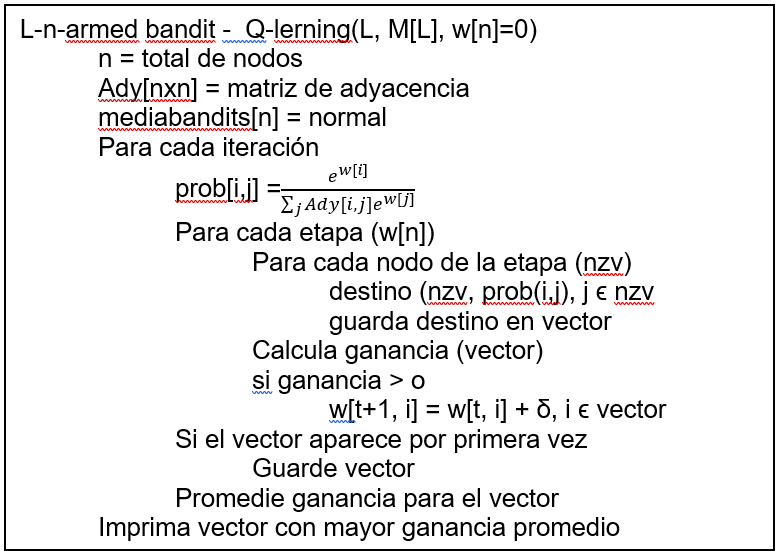
\includegraphics[scale=0.5]{PsQ-learning}
%	\caption{Pseudocódigo L-n-armed bandit – Q-learning}
%	\label{PsQ-learning}
%\end{figure}


En esta propuesta, la aplicación debe ir guardando en un arreglo cada una de las rutas nuevas que se van generando por iteración, junto con su ganancia calculada, porque si la ruta no es nueva, solo debe incrementar un contador que hace parte del mismo arreglo. De esta manera, al finalizar cualquier cantidad de iteraciones, se calculará la ganancia promedio para cada ruta generada, parámetro en el que se basa para seleccionar la ruta con mejor ganancia promedio y presentarla como la óptima.

Las pruebas correspondientes se presentan en el capítulo \ref{resul} donde se detallan los resultado que se fueron obteniendo en algoritmos previos y en los que finalmente se comparan.

\section{Pruebas}

\subsection{Generador de bandits}

Primero se probó el algoritmo que genera los \textit{bandits} para los nodos y aplica la fórmula de los promedios de las ganancias para entregar al final la acción con mejor valor asociado, dándole al algoritmo valores distorsionados que se encontraban entre una desviación estándar de 1 del valor asociado al \textit{bandit}. Este código se probó varias veces y siempre encontró el valor buscado. 

La figura \ref{AlgBandit} es el resultado gráfico de una corrida de este algoritmo con 400 iteraciones, donde la línea roja representa las ganancias que va encontrando en cada iteración y la línea horizontal que está ubicada en 1 representa el número del brazo que en promedio obtiene la mejor ganancia al finalizar las iteraciones, respuesta que corresponde exactamente con el \textit{bandit} que tiene asignado el mayor valor de ganancia real, de los 10 que se le dieron a escoger.

\begin{figure} [H]
    \label{Resul2}
	\centering
	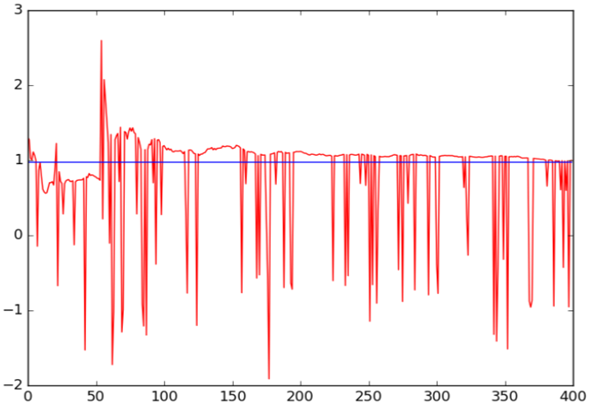
\includegraphics[scale=0.6]{AlgBandit}
	\caption{Resultado de la selección del mejor brazo usando la teoría de los \textit{bandits}}
	\label{AlgBandit}
\end{figure}

La oscilación de la línea roja se produce por la exploración que el algoritmo hace de otras alternativas diferentes a la que en cada momento parece ser la mejor. Tampoco dan los mismos valores aunque esté probando el mismo brazo, porque estos valores están siendo generado con una distribución normal, con media en uno real (que también fue aleatorio), pero dentro de una desviación estándar que en este caso fue de 1. 

\subsection{Generador de la matriz de adyacencia}

Posteriormente se implementó el código que genera las matrices de adyacencia del grafo por etapas. Estas matrices debían ser escalonadas, debían obedecer a los requisitos de precedencia de nodos entre etapas y debía tener al menos un 1 en cada fila para garantizar la conexión de las etapas. Este código también se probó varias veces y siempre arrojó resultados adecuados. Un ejemplo de este resultado se muestra en la figura \ref{MatrizAy}.

\begin{figure} [H]
    \label{Resul2}
	\centering
	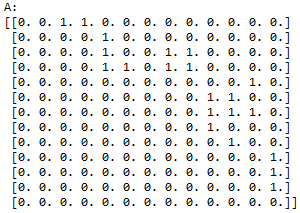
\includegraphics[scale=0.8]{MatrizAy}
	\caption{Resultado de la matriz de adyacencia para un grafo por etapas}
	\label{MatrizAy}
\end{figure}

\subsubsection{Generación de una ruta aleatoria}

Se implementó la fusión del algoritmo para la generación de la matriz de adyacencia, con el que genera los valores asociados a cada nodo o \textit{bandit}; el pseudocódigo correspondiente se probó con valores aleatorios, obteniendo siempre la matriz escalonada que se esperaba y los valores asociados a los \textit{bandits}.

Se le adicionó la funcionalidad de que tomara una ruta factible, teniendo en cuenta la matriz de adyacencia para tomar la información de los posibles vecinos de cada nodo. La pruebas que se hicieron funcionaron siempre correctamente.

Se procedió a probar que sobre la ruta que seleccionara calculara correctamente la ganancia real asociada, teniendo en cuenta el vector de valores generados para los \textit{bandits}, y la ganancia distorsionada asociada a esa misma ruta, teniendo en cuenta el nuevo vector de valores distorsionados de los \textit{bandits}, el cual se genera con números aleatorios que siguen una distribución normal con media en el elemento del primer vector, dentro de una desviación estándar de 1. Las pruebas para esta implementación siempre funcionaron correctamente.

\subsection{Encontrando la ruta óptima}

Aquí se dan tres momentos diferentes: Inicialmente el que ya está implementado, donde la escogencia del siguiente nodo de un camino, solo tiene que estar dentro del conjunto de vecinos del nodo actual, pero todos con la misma probabilidad de ser seleccionados; a este modelo le reconoceremos como Probabilidades Uniformes. Seguidamente se implementa la generación de la matriz de probabilidades de transición de pasar de un nodo a otro, la cual se basa en un fundamento matemático específico que se presentó en la sección \ref{mat} y del que se espera que converja a una única respuesta con la mejor ruta encontrada; a este le reconoceremos como Probabilidad Modelada. Finalmente, y en forma paralela con el desarrollo del algoritmo anterior, se implementa una funcionalidad que permite seleccionar la ruta que, durante todas las iteraciones, alcanzó el mayor promedio de ganancias, para entregarla como respuesta; este algoritmo lo reconoceremos como Promedio de Ganancias.

\subsection{Búsqueda con Probabilidad Uniforme}

Este algoritmo se construye básicamente, incluyendo un contador de iteraciones para que el algoritmo de generación de rutas factibles se ejecute una cantidad dada de veces determinada y una selección de la ruta que al final de las iteraciones hubiera obtenido la ganancia promedio, para entregarla como respuesta. 

Inicialmente los valores de la matriz de adyacencia y del vector de \textit{bandits} se generaron de forma aleatoria con las instrucciones que ya estaban probadas y que se describieron anteriormente, pero esto no permitía estimar la efectividad del algoritmo, porque, en muchos casos, no eran significativamente diferentes los valores asignados a los nodos y cualquier ruta era buena. 

\subsubsection{Grafo para las pruebas}

Se decide entonces trabajar con un grafo de 5 etapas y 13 nodos, dispuestos como se ve en la figura \ref{Grafomodelo}, pero no necesariamente con esas aristas, es decir, con matriz de adyacencia aleatoria, así como los valores de sus \textit{bandits}, pero obligando a que uno de ellos por etapa tuviese un mayor valor que los demás, para favorecer la ruta mejor y así verificar si estaba funcionando.

\begin{figure}[h]
  \centering
    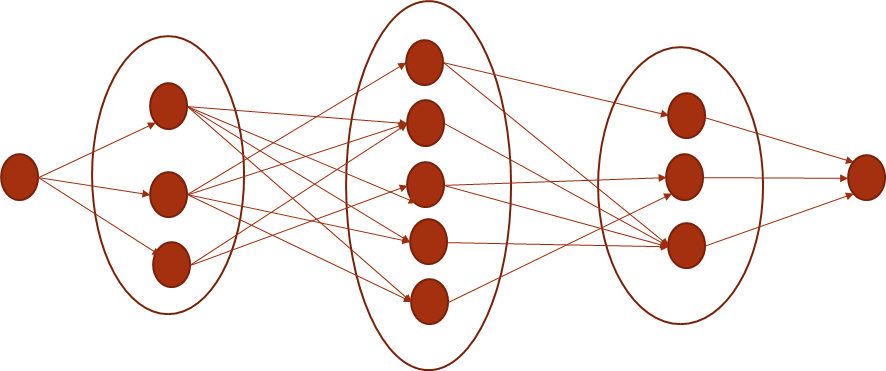
\includegraphics[scale=0.5]{GrafoModelo.png}
  \caption[Grafo Modelo]{Grafo Modelo con 5 etapas y 13 nodos}
  \label{Grafomodelo}
\end{figure}

De otra parte, era importante saber cómo se comportaba el algoritmo, al ejecutarlo varias veces, dejando fijos los datos de entrada correspondientes al grafo que se quería evaluar, por lo que de aquí en adelante no se generaron más matrices de adyacencia ni vectores reales de los \textit{bandits} aleatorios, sino que se dejaron los siguientes:

\renewcommand{\arraystretch}{0.5}
%\begin{equation}
A = 
$\begin{bmatrix}
%\hspace{2cm}

0, 0, 1,  1,  0,  0,  0,  0,  0,  0,  0,  0,  0\\
0, 0, 0,  0,  1,  0,  0,  0,  0,  0,  0,  0,  0\\
0, 0, 0,  0,  1,  0,  0,  1,  1,  0,  0,  0,  0\\
0, 0, 0,  0,  1,  1,  0,  1,  1,  0,  0,  0,  0\\
0, 0, 0,  0,  0,  0,  0,  0,  0,  0,  0,  1,  0\\
0, 0, 0,  0,  0,  0,  0,  0,  0,  1,  1,  0,  0\\
0, 0, 0,  0,  0,  0,  0,  0,  0,  1,  1,  1,  0\\
0, 0, 0,  0,  0,  0,  0,  0,  0,  1,  0,  0,  0\\
0, 0, 0,  0,  0,  0,  0,  0,  0,  0,  1,  0,  0\\
0, 0, 0,  0,  0,  0,  0,  0,  0,  0,  0,  1,  0\\
0, 0, 0,  0,  0,  0,  0,  0,  0,  0,  0,  1,  0\\
0, 0, 0,  0,  0,  0,  0,  0,  0,  0,  0,  1,  0\\
0, 0, 0,  0,  0,  0,  0,  0,  0,  0,  0,  0,  0
\end{bmatrix}$

%\end{equation}

%\begin{figure}
%	\centering
%	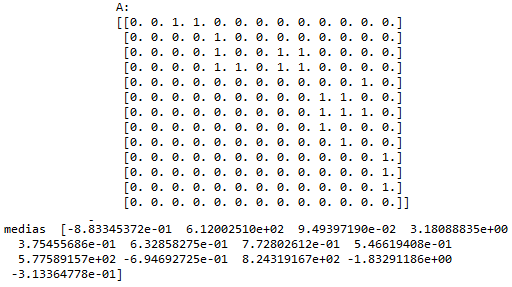
\includegraphics[scale=1]{MatrizAyBandits2}
%	\caption{Matriz y bandit generados}
%	\label{AyB}
%\end{figure}

B = [- 0.833e-01, 6.12e+02, 9.49e-02, 3.18e+00, 3.75e-01, 6.33e-01, 7.73e-01, 5.47e-01, 5.77e+02, -6.95e-01, 8.23e+02, -1.83e+00, -3.13e-01]

\subsubsection{Resultados probabilidad uniforme}

El algoritmo cuyo pseudocódigo se presentó en el cuadro \ref{PsUniforme}, se ejecutó con 99 intervalos de tiempo. La figura \ref{fig:uniforme} muestra uno de los resultados. 

\begin{figure}[H]
	\centering
	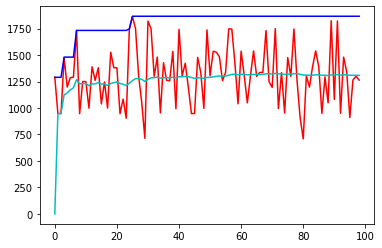
\includegraphics[scale=1]{Uniforme}
	\caption{Resultado con probabilidad uniforme}
	\label{fig:uniforme}
\end{figure}

En esta gráfica, la curva superior azul corresponde a la ganancia de la mejor ruta probada hasta el momento, calculada con el valor real de los \textit{bandits} o medias asignadas a cada uno; en la curva más inestable se presentan las ganancias obtenidas en cada instante de tiempo por la ruta seleccionada, calculada con los valores distorsionados de los \textit{bandits}, que fueron generados alrededor del vector B de las medias, con una desviación estándar de 1; y en la curva inferior verdosa se muestra el promedio acumulado de estas ganancias, el cual converge a un único valor a través del tiempo, pero no trata de acercarse al valor real.

\subsection{Resultados probabilidad modelada}

Para 33 iteraciones, T=33 en el algoritmo que se muestra en el cuadro \ref{Pseudo}, para las cales se pueden apreciar los valores que van tomado sus variables para construir la matriz de probabilidades de transición, la ganancia promedio generada por el algoritmo, convergió rápidamente hacia el valor de la mejor ganancia real como se puede apreciar en la figura \ref{Resul2}. 

\begin{figure} [H]
	\centering
	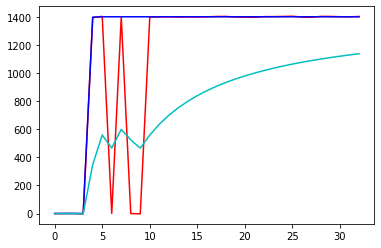
\includegraphics[scale=1]{Resul2}
	\caption{Resultado con probabilidad ponderada semialeatorio}
	\label{Resul2}
\end{figure}

En esta gráfica, al igual que en la del modelo anterior, la curva superior azul corresponde a la ganancia de la mejor ruta probada hasta el momento, calculada con el valor real de los \textit{bandits} o medias asignadas a cada uno; en la curva más inestable se presentan las ganancias obtenidas en cada instante de tiempo por la ruta seleccionada, calculada con los valores distorsionados de los \textit{bandits}, que fueron generados alrededor del vector B de las medias, con una desviación estándar de 1; y en la curva inferior verdosa se muestra el promedio acumulado de estas ganancias.

\subsection{Resultados selección de la ruta con mayor ganancia promedio}

También se implementa un algoritmo que evalúa el resultado al estilo de \textit{Q-learning}, pero donde la selección no se hace sobre un conjunto de acciones, sino sobre un conjunto de rutas de acciones de las que ha explorado alguna vez, cuyo pseudocódigo se muestra en el cuadro algorítmico \ref{PsQ-learning}. Para garantizar una comparación válida, este algoritmo se incorpora en el mismo código del algoritmo anteriormente presentado, lo que asegura que se manejan los mismos datos y que las decisiones que se toman de forma aleatoria serán las mismas. 

El 100\% de las veces que se probó, encontró la ruta óptima. No se generan gráficas para este algoritmo, puesto que no se haya un único promedio de ganancias, sino que se promedia para cada una de las rutas que el algoritmo encuentra, de forma que el criterio de selección de la ruta óptima no tiene que ver con convergencia alguna.

%\section{Pruebas de los algoritmos propuestos} 

%\section{GENERACIÓN DE DATOS ALEATORIOS}
%Al rededor de los valores dados a cada uno de los nodos del grafo, la aplicación genera valores distorsionados con una diferencia de más o menos uno, generados en forma aleatoria, siendo diferentes los valores que se obtienen en cada ejecución.

%Así mismo, todos los nodos tienen la misma probabilidad de ser elegidos cuando se hace la primera corrida, así que la aplicación hace las selecciones en cada etapa, mediante la generación de un valor aleatorio con distribución uniforme; para los demás tiempos de corridas, en que los nodos ya cuentan con valore asociados, el nodo que selecciona dentro de los vecinos de un nodo cualquiera, atendiendo a las probabilidades de transición que se le ofrecen, en forma de ruleta donde el ancho de las franjas para cada opción es equivalente al la probabilidad misma.

%Estos valores distorsionados, con los que realmente decide el jugador y, por ende, trabaja la aplicación, han sido calculados sumándole al número que indica la recompensa real, una cantidad aleatoria generada con una distribución normal con media en 0 y una desviación estándar de 1, es decir que se le suma a la media una cantidad entre -1 y +1.

\section{Comparación entre Probabilidad Modelada y Mayor ganancia promedio} 

Estos dos algoritmos han logrado encontrar la ruta óptima del grafo elegido. Aquí presentamos los resultados de los dos, ejecutándolos en el mismo programa, para que los valores que se generan aleatoriamente sean los mismos y darle de esta forma validez a la comparación.

Se toma el grafo modelo que se presenta en la figura \ref{Grafomodelo} con su matriz de adyacencia fija, así como los valores para sus \textit{bandits}, que ya se escribieron anteriormente, de forma que cualquier resultada se pueda comparar con los de otros algoritmos y con ejecuciones posteriores del mismo algoritmo. Se le da libertad al algoritmo para generar aleatoriamente los valores distorsionados de los \textit{bandit} que simula la incertidumbre del ejercicio, al no conocerse los valores reales. Finalmente, el algoritmo decide los nodos que selecciona en cada etapa y, así, las rutas a seguir también serán aleatorias.

La decisión de usar una generación de números aleatorios que siguen una distribución normal con media en cero y desviación estándar en 1, es porque es la utilizada en la literatura de aprendizaje por refuerzo \citep{sutton1992reinforcement}, con la cual se ha probado el funcionamiento del modelo de decisión n-armed bandit. 

%Para demostrar la importancia que tiene el modelo de la generación de probabilidades de transición de estados entre los nodos, se corrió una aplicación donde los nodos se seleccionan todo el tiempo al azar, respetando las posibilidades de adyacencia del grafo, y se comparan sus resultados con una ejecución del algoritmo que genera y tiene en cuenta las probabilidades mencionadas.

Con un $\delta$ de aprendizaje de 0.0003 multiplicado por el valor de la ganancia o recompensa de la ruta utilizada, Se hicieron 10 corridas al algoritmo de probabilidades de transición, el cual permite que, a lo largo de todas las corridas o ejecuciones del algoritmo, se vaya aumentando la probabilidad de que cada nodo sea escogido.

Para cada ejecución se ha seleccionado la última respuesta que arrojó la aplicación en cada una de las dos modalidades expuestas donde, para el caso del algoritmo de Probabilidad modelada, fue la que se obtuvo cuando el algoritmo convergió, haciendo uso de la fórmula \ref{model2}, como se explicó en la sección \ref{implemodprob}, mientras que para el caso de algoritmo de Mayor ganancia promedio, esta respuesta es la que se va dando al terminar cada iteración. 

Los resultados obtenidos se muestran en la tabla \ref{tabComUP}, en los cuales se puede establecer que el 70\% de las veces que se probó el algoritmo de Probabilidad modelada, encontró la ruta óptima y que el 100\% de las veces que se probó el algoritmo de Mayor ganancia promedio, este encontró la ruta óptima.

\renewcommand{\arraystretch}{0.5}
\begin{table}[H] 
\centering
\caption{Comparación de resultados de los dos enfoques} \begin{tabular}{ccc}
\hline
\begin{tabular}[c]{@{}c@{}}Número de \\ Corrida\end{tabular} & \begin{tabular}[c]{@{}c@{}}Con el modelo \\ de probabilidades\end{tabular} & \begin{tabular}[c]{@{}c@{}}Con el simulador \\ de bandits de vectores\end{tabular} \\[0.5ex] \hline
1                           & {[}0, 2, 4, 11, 12{]}                               & {[}0, 2, 4, 11, 12{]}                                       \\
2                           & {[}0, 2, 5, 11, 12{]}                               & {[}0, 2, 4, 11, 12{]}                                       \\
3                           & {[}0, 2, 4, 11, 12{]}                               & {[}0, 2, 4, 11, 12{]}                                       \\
4                           & {[}0, 2, 4, 11, 12{]}                               & {[}0, 2, 4, 11, 12{]}                                       \\
5                           & {[}0, 2, 4, 11, 12{]}                               & {[}0, 2, 4, 11, 12{]}                                       \\
6                           & {[}0, 2, 4, 11, 12{]}                               & {[}0, 2, 4, 11, 12{]}                                       \\
7                           & {[}0, 2, 4, 11, 12{]}                               & {[}0, 2, 4, 11, 12{]}                                       \\
8                           & {[}0, 2, 7, 11, 12{]}                               & {[}0, 2, 4, 11, 12{]}                                       \\
9                           & {[}0, 2, 4, 11, 12{]}                               & {[}0, 2, 4, 11, 12{]}                                       \\
10                          & {[}0, 2, 7, 11, 12{]}                               & {[}0, 2, 4, 11, 12{]}                                 
\end{tabular}
\label{tabComUP}
\end{table}

Adicionalmente a los resultados que se muestran en la tabla \ref{tabComUP}, se pueden observar las figuras generadas por la aplicación el la figura \ref{fig:grafi}. Allí, la curva superior, que se dejó en color verde, representa la ganancia de la mejor ruta probada hasta ese momento, calculada con los valores reales de los \textit{bandits} ya dados en el vector B. Esto permite que el software sea el que estime la mejor ruta, de un conjunto aleatorio de nodos, sin una intervención manual, ya que hacer este cálculo equivaldría a una búsqueda exhaustiva en árbol, lo que puede llegar a ser muy dispendioso.

Seguidamente, en la curva más variable (roja) se presentan las ganancias obtenidas en cada una de las iteraciones por la ruta allí seleccionada, calculada con los valores distorsionados de los \textit{bandits}, que fueron generados alrededor de las medias reales con desviación estándar de 1. 

Y, por último, en la curva inferior (azul) se muestra el promedio acumulado de estas ganancias, el cual converge a un único valor a través del tiempo y se espera que se acerque al valor real de la mejor ruta, representado en la línea superior.

Se ejecuta el código 10 veces consecutivas para obtener una estimación inicial de su efectividad, cada vez con 999 iteraciones.

Los resultados obtenidos entregan el vector de nodos de las L etapas que ofrece la mayor ganancia, como es [0,2,4,11,12], para los dos modelos, que, en este caso, se puede verificar manualmente.

Como en otras oportunidades, se obtiene solo un porcentaje de siete de diez ejecuciones que llevan a la respuesta correcta siguiendo el procedimiento de generación aproximada de la matriz de transición de probabilidades, como se puede apreciar en la figura compuesta \ref{fig:grafi} y en la tabla \ref{tabComUP}. %el apéndice \ref{resultProb10}%.

\begin{figure} 
    \centering
    \begin{subfigure}[b]{0.39\textwidth}
        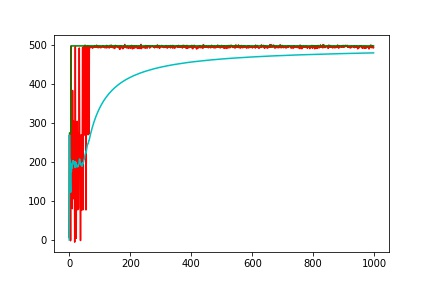
\includegraphics[width=\textwidth]{grafi1.jpg}
        %\caption{A gull}
        \label{fig:gull}
    \end{subfigure}
    \vspace{0.5 mm}
    ~ %add desired spacing between images, e. g. ~, \quad, \qquad, \hfill etc. 
      %(or a blank line to force the subfigure onto a new line)
    \begin{subfigure}[b]{0.39\textwidth}
        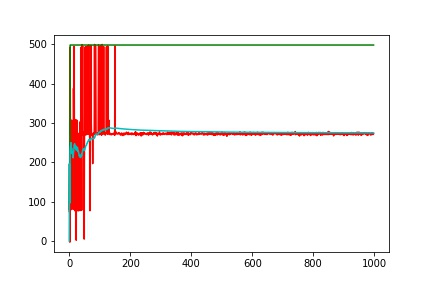
\includegraphics[width=\textwidth]{grafi2.jpg}
        %\caption{A tiger}
        \label{fig:tiger}
    \end{subfigure}
    ~ %add desired spacing between images, e. g. ~, \quad, \qquad, \hfill etc. 
    %(or a blank line to force the subfigure onto a new line)
    \begin{subfigure}[b]{0.39\textwidth}
        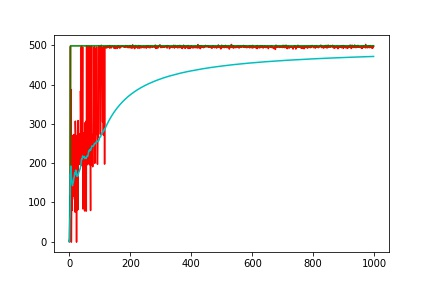
\includegraphics[width=\textwidth]{grafi3.jpg}
        %\caption{A mouse}
        \label{fig:mouse}
    \end{subfigure}
    \begin{subfigure}[b]{0.39\textwidth}
        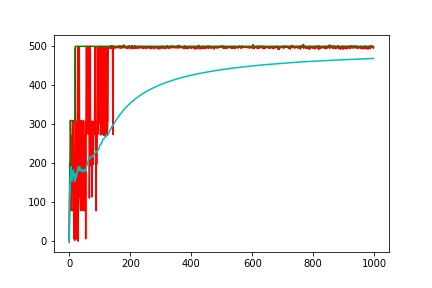
\includegraphics[width=\textwidth]{grafi4.jpg}
        %\caption{A tiger}
        \label{fig:tiger}
    \end{subfigure}
        \begin{subfigure}[b]{0.39\textwidth}
        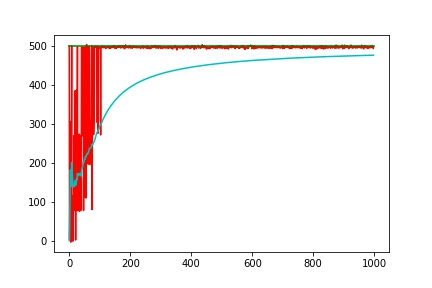
\includegraphics[width=\textwidth]{grafi5.jpg}
        %\caption{A gull}
        \label{fig:gull}
    \end{subfigure}
    ~ %add desired spacing between images, e. g. ~, \quad, \qquad, \hfill etc. 
      %(or a blank line to force the subfigure onto a new line)
    \begin{subfigure}[b]{0.39\textwidth}
        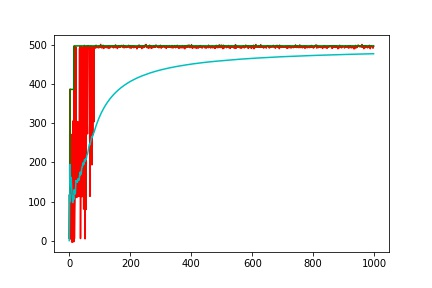
\includegraphics[width=\textwidth]{grafi6.jpg}
        %\caption{A tiger}
        \label{fig:tiger}
    \end{subfigure}
    ~ %add desired spacing between images, e. g. ~, \quad, \qquad, \hfill etc. 
    %(or a blank line to force the subfigure onto a new line)
    \begin{subfigure}[b]{0.39\textwidth}
        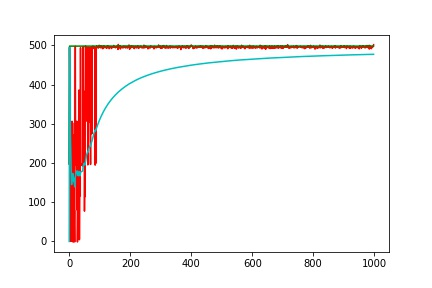
\includegraphics[width=\textwidth]{grafi7.jpg}
        %\caption{A mouse}
        \label{fig:mouse}
    \end{subfigure}
    \begin{subfigure}[b]{0.39\textwidth}
        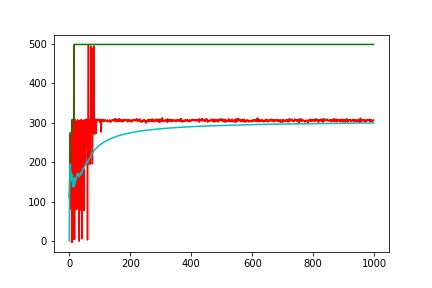
\includegraphics[width=\textwidth]{grafi8.jpg}
        %\caption{A tiger}
        \label{fig:tiger}
    \end{subfigure}
    \begin{subfigure}[b]{0.39\textwidth}
        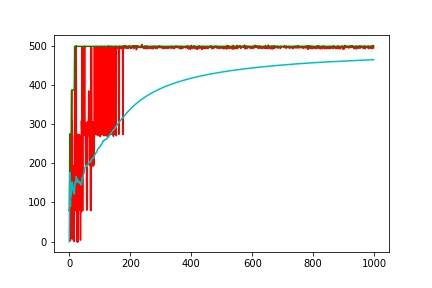
\includegraphics[width=\textwidth]{grafi9.jpg}
        %\caption{A mouse}
        \label{fig:mouse}
    \end{subfigure}
    \begin{subfigure}[b]{0.39\textwidth}
        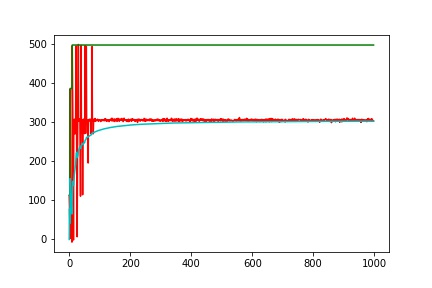
\includegraphics[width=\textwidth]{grafi10.jpg}
        %\caption{A tiger}
        \label{fig:tiger}
    \end{subfigure}    
    \caption{Ejecución algoritmo Probabilidad Modelada}\label{fig:grafi}
\end{figure}

%el anexo \ref{resultBandit10}
De otra parte, en la tabla \ref{tabComUP} también se aprecian los resultados de las 10 ejecuciones, todas con la respuesta correctas, junto con los arreglos donde, cada uno de los vectores que representa una ruta, hallada alguna vez por el algoritmo, tiene una ganancia promedio asociada y el número de veces que ha sido seleccionado.

No se presentan gráficas para mostrar la eficiencia de este aplicativo, puesto que no depende de alguna convergencia, sino que, únicamente, obedece a la fórmula de promedio de ganancias que ofrece el aprendizaje por refuerzo.

%Un resumen de los resultados obtenidos en estas dos variantes del modelo se muestra en la tabla \ref{tabComUP}. 
Para el ejercicio propuesto el valor correcto al que se esperaba llegar era el vector [0, 2, 4, 11, 12], que es precisamente el que más se repite.

%En los apéndices \ref{run1}, \ref{resultProb10} y \ref{resultBandit10} se detallan resultados que arroja la ejecución de los algoritmos presentados.
El análisis de estos dos algoritmos deberá hacerse desde una prueba con un grafo de mayor complejidad, donde se espera que tenga un mejor desempeño el algoritmo Probabilidad Modelada, puesto que no requiere almacenar la información de las rutas, lo que sería una desventaja para el algoritmo de Mayor ganancia promedio que maneja un arreglo en cuyos registros se tiene la información de la ruta, la ganancia promedio y el número de veces que ha salido.

Además el algoritmo tiene la característica del Aprendizaje por refuerzo de la exploración, la cual le permite, de vez en cuando, visitar otras rutas con nodos que quizás no tenga una alta probabilidad de ser seleccionados pero que puede ser parte de una mejor respuesta que la que se esté evaluando.

Se procede a establecer como influye el valor de deltha, únicamente, en el algoritmo de Probabilidad modelada, para dar una recomendación fundamentada sobre le valor que conviene utilizar.

\section{Comparación al cambiar el coeficiente de aprendizaje}

Se retoman aquí las fórmulas con las que se consigue que el autómata aprenda y genere una matriz de probabilidades de transición entre nodos, para contextualizar a lo que se refiere el llamado \textbf{coeficiente de aprendizaje}. En la fórmula de probabilidades \ref{prob4} se observa que el exponente es una posición de un vector que se va actualizando, de acuerdo al resultado de ganancia o pérdida de cada ejercicio, de la forma que se muestra en la fórmula \ref{exponente4}.
\begin{eqnarray}\label{prob4}
P(i \to j) = \frac{e^{v_j}}{\sum_k A_{i,k} e^{v_k}},
\end{eqnarray}
\begin{eqnarray}\label{exponente4}
v_j(\tau + 1) = v_j(\tau) + \delta,
\end{eqnarray}

El valor de $\delta$ en esta función, fue seleccionado inicialmente con valores entre 0.1 y 0.9, los que son positivos en caso de ganancia y negativos en caso de pérdida, para motivar o desmotivar al autómata para que en el paso siguiente seleccionen los nodos que reciben el refuerzo. Las diferencias normalizadas que se encontraron entre la ganancia real y cada una de las ganancias que en promedio se obtuvieron en 100 iteraciones para cada combinación de parámetros se ve en la tabla \ref{tabla10}.

\begin{table}[H]
\small
\caption{Resultados con Deltha en décimas}
\begin{tabular}{|c|r|r|r|r|r|r|r|r|r|r|}
\hline
\multicolumn{1}{|l|}{Deltha} & \multicolumn{10}{c|}{Iteraciones} \\ \hline
\multicolumn{1}{|l|}{}       & \multicolumn{1}{c|}{100} & \multicolumn{1}{c|}{200} & \multicolumn{1}{c|}{300} & \multicolumn{1}{c|}{400} & \multicolumn{1}{c|}{500} & \multicolumn{1}{c|}{600} & \multicolumn{1}{c|}{700} & \multicolumn{1}{c|}{800} & \multicolumn{1}{c|}{900} & \multicolumn{1}{c|}{1000} \\ \hline
0,1                          & 0.715                    & 0.715                    & 0.715                    & 0.715                    & 0.715                    & 0.715                    & 0.715                    & 0.715                    & 0.715                    & 0.715                     \\ \hline
0,2                          & 0.695                    & 0.695                    & 0.695                    & 0.695                    & 0.695                    & 0.695                    & 0.695                    & 0.695                    & 0.695                    & 0.695                     \\ \hline
0,3                          & 0.676                    & 0.676                    & 0.676                    & 0.676                    & 0.676                    & 0.676                    & 0.676                    & 0.676                    & 0.676                    & 0.676                     \\ \hline
0,4                          & 0.656                    & 0.656                    & 0.656                    & 0.656                    & 0.656                    & 0.656                    & 0.656                    & 0.656                    & 0.656                    & 0.656                     \\ \hline
0,5                          & 0.637                    & 0.637                    & 0.637                    & 0.637                    & 0.637                    & 0.637                    & 0.637                    & 0.637                    & 0.637                    & 0.637                     \\ \hline
0,6                          & 0.618                    & 0.618                    & 0.618                    & 0.618                    & 0.618                    & 0.618                    & 0.618                    & 0.618                    & 0.618                    & 0.618                     \\ \hline
0,7                          & 0.598                    & 0.598                    & 0.598                    & 0.598                    & 0.598                    & 0.598                    & 0.598                    & 0.598                    & 0.598                    & 0.598                     \\ \hline
0,8                          & 0.579                    & 0.579                    & 0.579                    & 0.579                    & 0.579                    & 0.579                    & 0.579                    & 0.579                    & 0.579                    & 0.579                     \\ \hline
0,9                          & 0.559                    & 0.559                    & 0.559                    & 0.559                    & 0.559                    & 0.559                    & 0.559                    & 0.559                    & 0.559                    & 0.559                     \\ \hline
\end{tabular}
\label{tabla10}
\end{table}
Los rangos de diferencia superan el 50\%, independientemente de la cantidad de iteraciones que se ejecuten, por lo que se procede a probar valores de deltha más pequeños, es decir, en magnitudes de centésimas, milésimas y diezmilésimas, sin conseguir mejorar en los resultados de las ganancias, como se puede apreciar en la tabla \ref{tabla100_10000}.

\begin{table}[H]
\small
\caption{Resultados con Deltha en centésimas, milésimas y diezmilésimas}
\begin{tabular}{rrrrrrrrrrr}
\multicolumn{1}{l}{Deltha} & \multicolumn{10}{c}{Iteraciones}                                                                                                                                                                                                    \\
\multicolumn{1}{l}{}       & 100                  & 200                  & 300                  & 400                  & 500                  & 600                  & 700                  & 800                  & 900                  & 1000                 \\
0.01                       & 0.697                & 0.697                & 0.671                & 0.695                & 0.675                & 0.677                & 0.661                & 0.694                & 0.654                & 0.692                \\
0.02                       & 0.707                & 0.686                & 0.628                & 0.583                & 0.565                & 0.605                & 0.661                & 0.751                & 0.760                & 0.809                \\
0.03                       & 0.615                & 0.698                & 0.763                & 0.744                & 0.742                & 0.734                & 0.777                & 0.512                & 0.813                & 0.819                \\
0.04                       & 0.646                & 0.651                & 0.533                & 0.783                & 0.812                & 0.800                & 0.505                & 0.495                & 0.815                & 0.820                \\
0.05                       & 0.816                & 0.720                & 0.780                & 0.795                & 0.504                & 0.484                & 0.483                & 0.798                & 0.817                & 0.492                \\
0.06                       & 0.607                & 0.475                & 0.806                & 0.555                & 0.809                & 0.537                & 0.459                & 0.817                & 0.819                & 0.476                \\
0.07                       & 0.725                & 0.764                & 0.774                & 0.810                & 0.824                & 0.514                & 0.824                & 0.831                & 0.837                & 0.822                \\
0.08                       & 0.654                & 0.806                & 0.450                & 0.472                & 0.492                & 0.476                & 0.490                & 0.421                & 0.471                & 0.466                \\
0.09                       & 0.756                & 0.765                & 0.502                & 0.604                & 0.486                & 0.820                & 0.780                & 0.775                & 0.827                & 0.835                \\
\multicolumn{1}{l}{}       & \multicolumn{1}{l}{} & \multicolumn{1}{l}{} & \multicolumn{1}{l}{} & \multicolumn{1}{l}{} & \multicolumn{1}{l}{} & \multicolumn{1}{l}{} & \multicolumn{1}{l}{} & \multicolumn{1}{l}{} & \multicolumn{1}{l}{} & \multicolumn{1}{l}{} \\
\multicolumn{1}{l}{Deltha} & \multicolumn{10}{c}{Iteraciones}                                                                                                                                                                                                    \\
\multicolumn{1}{l}{}       & 100                  & 200                  & 300                  & 400                  & 500                  & 600                  & 700                  & 800                  & 900                  & 1000                 \\
0.001                      & 0.690                & 0.699                & 0.705                & 0.713                & 0.705                & 0.704                & 0.708                & 0.727                & 0.713                & 0.698                \\
0.002                      & 0.702                & 0.710                & 0.706                & 0.715                & 0.716                & 0.696                & 0.682                & 0.680                & 0.696                & 0.714                \\
0.003                      & 0.647                & 0.719                & 0.682                & 0.692                & 0.699                & 0.700                & 0.709                & 0.691                & 0.687                & 0.659                \\
0.004                      & 0.711                & 0.721                & 0.697                & 0.694                & 0.688                & 0.687                & 0.671                & 0.691                & 0.681                & 0.693                \\
0.005                      & 0.763                & 0.691                & 0.710                & 0.682                & 0.688                & 0.686                & 0.667                & 0.664                & 0.684                & 0.689                \\
0.006                      & 0.692                & 0.726                & 0.693                & 0.692                & 0.716                & 0.689                & 0.654                & 0.680                & 0.647                & 0.605                \\
0.007                      & 0.730                & 0.695                & 0.696                & 0.680                & 0.680                & 0.656                & 0.674                & 0.626                & 0.706                & 0.656                \\
0.008                      & 0.728                & 0.651                & 0.708                & 0.669                & 0.668                & 0.686                & 0.681                & 0.710                & 0.692                & 0.665                \\
0.009                      & 0.707                & 0.695                & 0.644                & 0.691                & 0.640                & 0.717                & 0.714                & 0.614                & 0.703                & 0.692                \\
\multicolumn{1}{l}{}       & \multicolumn{1}{l}{} & \multicolumn{1}{l}{} & \multicolumn{1}{l}{} & \multicolumn{1}{l}{} & \multicolumn{1}{l}{} & \multicolumn{1}{l}{} & \multicolumn{1}{l}{} & \multicolumn{1}{l}{} & \multicolumn{1}{l}{} & \multicolumn{1}{l}{} \\
\multicolumn{1}{l}{Deltha} & \multicolumn{10}{c}{Iteraciones}                                                                                                                                                                                                    \\
\multicolumn{1}{l}{}       & 100                  & 200                  & 300                  & 400                  & 500                  & 600                  & 700                  & 800                  & 900                  & 1000                 \\
0.0001                     & 0.708                & 0.689                & 0.728                & 0.718                & 0.693                & 0.709                & 0.700                & 0.694                & 0.709                & 0.699                \\
0.0002                     & 0.684                & 0.697                & 0.718                & 0.696                & 0.710                & 0.734                & 0.700                & 0.706                & 0.708                & 0.699                \\
0.0003                     & 0.718                & 0.683                & 0.693                & 0.699                & 0.706                & 0.715                & 0.699                & 0.707                & 0.715                & 0.696                \\
0.0004                     & 0.748                & 0.717                & 0.704                & 0.707                & 0.710                & 0.745                & 0.705                & 0.705                & 0.707                & 0.713                \\
0.0005                     & 0.686                & 0.692                & 0.705                & 0.733                & 0.700                & 0.706                & 0.709                & 0.691                & 0.704                & 0.717                \\
0.0006                     & 0.649                & 0.742                & 0.703                & 0.711                & 0.699                & 0.685                & 0.717                & 0.706                & 0.707                & 0.706                \\
0.0007                     & 0.752                & 0.723                & 0.733                & 0.706                & 0.700                & 0.701                & 0.688                & 0.709                & 0.697                & 0.722                \\
0.0008                     & 0.682                & 0.725                & 0.704                & 0.706                & 0.720                & 0.690                & 0.700                & 0.712                & 0.705                & 0.709                \\
0.0009                     & 0.718                & 0.680                & 0.708                & 0.691                & 0.694                & 0.702                & 0.702                & 0.714                & 0.688                & 0.698               
\end{tabular}
\label{tabla100_10000}
\end{table}
Aquí se puede apreciar que, a pesar de disminuir notablemente los valores de deltha, se siguen obteniendo valores muy altos para la diferencia de las ganancias, con errores superiores al 40\%. Los promedios de estas diferencias se presentan en la tablas \ref{delthas_0000}

\begin{table}[H]
\centering
%\small
\caption{Promedios de los resultados variando décimas en Deltha}
\begin{tabular}{llll}
\multicolumn{4}{c}{\textbf{PROMEDIOS DE ERROR EN GANANCIAS}}                                                  \\
\textbf{Décimas}          & \textbf{Centésimas}       & \textbf{Milésimas}        & \textbf{Diezmilésimas}    \\
\multicolumn{1}{r}{0.637} & \multicolumn{1}{r}{0.675} & \multicolumn{1}{r}{0.690} & \multicolumn{1}{r}{0.706}
\end{tabular}
\label{delthas_0000}
\end{table}

Se procede a crear un deltha ($\delta$) autoajustable, que dependa del valor de la ganancia que recibe la ruta probada, de forma que, inclusive, el signo se ajustará cuando hayan pérdidas. Se involucra una nueva variable Gamma ($\gamma$) que, al multiplicarse por la ganancia o recompensa recibida al final del camino, va a dar el valor $\delta$ para la ecuación \ref{exponente4}.

Se hace necesario tomar valores para $\gamma$ del orden de diezmilésimas, para que al multiplicarlo por la ganancia. que para este ejemplo alcanza valores cercanos a 500 unidades, se obtengan valores de $\delta$ inferiores a uno.

\begin{table}[H]
\centering
%\small
\caption{Promedios de distancias usando Gamma}
\begin{tabular}{cllllll}
%\multicolumn{7}{c}{DISTANCIAS EN GANANCIAS PROMEDIO}                                                                                   %                                            \\
GAMA                 & \multicolumn{6}{c}{ITERACIONES}                                                                                                                            \\
\multicolumn{1}{l}{} & \multicolumn{1}{c}{100} & \multicolumn{1}{c}{300} & \multicolumn{1}{c}{500} & \multicolumn{1}{c}{700} & \multicolumn{1}{c}{900} & \multicolumn{1}{c}{1000} \\
0,00001              & 0,368                   & 0,36                    & 0,344                   & 0,328                   & 0,322                   & 0,272                    \\
0,00025              & 0,102                   & 0,044                   & 0,034                   & 0,066                   & 0,052                   & 0,042                    \\
0,00050              & 0,05                    & 0,078                   & 0,082                   & 0,072                   & 0,082                   & 0,074                    \\
0,00075              & 0,08                    & 0,092                   & 0,086                   & 0,09                    & 0,078                   & 0,09                     \\
0,00099              & 0,092                   & 0,102                   & 0,084                   & 0,084                   & 0,1                     & 0,106                   
\end{tabular}
\end{table}
\label{experimento1}

Los resultados mejoraron considerablemente, obteniendo un promedio en el error para esta tabla del 13\%, o del 8\% eliminando la primera fila donde se encuentran los valores más altos. También, se puede notar en esta tabla que los errores están influidos tanto por el valor de Gamma, como por el número de iteraciones que se ejecutan.

Se procede entonces a hacer el análisis correspondiente para establecer experimentalmente la relación que aquí se intuye.

\section{Diseño de experimentos}

La variable dependiente para este conjunto de experimentos, corresponde a la diferencia entre la ganancia máxima y la ganancia obtenida en la ejecución. Para estimar el error que se está generando a partir de esta diferencia, se normaliza esta última dividiéndola en el valor de la ganancia máxima, de forma que se obtengan valores entre cero y uno.

Los experimentos se diseñan teniendo en cuenta que las variables independientes corresponden a 
\begin{itemize}
    \item Coeficiente del factor de aprendizaje $\gamma$
    \item Número de iteraciones
\end{itemize}

Para el control o validez interna se ha de comprobar que las variables, aquí definidas como independientes, son las que realmente influyen en las dependientes, y no factores externos como la aleatoriedad. Se tomarán los resultados de 100 experimentos con cada uno de los valores de control sobre las variables independientes.

La técnica que se usa en este experimento es la simulación. Es un instrumento objetivo, confiable y válido. La validez es alta, puesto que el computador siempre tratará los valores de la misma manera; se espera que con un mismo valor de variables independientes se obtengan resultados similares en las variables dependientes.

Se harán cálculos de medias, varianzas y de análisis de varianza (ANOVA) que permita concluir la forma en que cada variable independiente influye en la dependiente.

\subsection{Experimento uno}
Se plantea una prueba que permita estimar si el valor de Gamma y el número de iteraciones son factores que afectan la diferencia normalizada entre la ganancia obtenida en cada ejecución del algoritmo y la ganancia óptima esperada.

Utilizando los datos de la tabla \ref{experimento1}, se obtienen promedios y varianza para cada fila y para cada columna, como se presenta en la tabla \ref{media_var_1}.

\begin{table}[H]
\centering
%\small
\caption{Medias y varianzas en Promedios de distancias usando Gamma}
\begin{tabular}{rrr}
\multicolumn{1}{l}{}            & \multicolumn{1}{c}{\textit{\textbf{PROMEDIO}}} & \multicolumn{1}{c}{\textit{\textbf{VARIANZA}}} \\ 
\multicolumn{1}{l}{GAMMA}       & \multicolumn{1}{l}{}                           & \multicolumn{1}{l}{}                           \\
0.00001                         & 0.3323                                         & 0.001188                                       \\
0.00025                         & 0.0567                                         & 0.000611                                       \\
0.00050                         & 0.0730                                         & 0.000144                                       \\
0.00075                         & 0.0860                                         & 0.000034                                       \\
0.00099                         & 0.0947                                         & 0.000089                                       \\
\multicolumn{1}{l}{ITERACIONES} & \multicolumn{1}{l}{}                           & \multicolumn{1}{l}{}                           \\
100                             & 0.1384                                         & 0.016855                                       \\
300                             & 0.1352                                         & 0.016273                                       \\
500                             & 0.126                                          & 0.015322                                       \\
700                             & 0.128                                          & 0.012590                                       \\
900                             & 0.1268                                         & 0.012201                                       \\
1000                            & 0.1168                                         & 0.008087                                      
\end{tabular}
\label{media_var_1}
\end{table}

Aquí se puede notar que el incremento en el valor de $\gamma$, no necesariamente produce un incremento o decremento en el promedio de las ganancias, mientras que cada vez que se aumentó el número de iteraciones en el experimento, se mejoró, es decir, disminuyó el promedio de las ganancias.

Los valores de las varianzas para cada valor de gamma es inferior a los de las varianzas para cada cifra de iteraciones, lo que indica que para el cambio de cantidad de iteraciones para calcular el promedio de ganancias en cada valor de gama no tiene tanta importancia como el cambio de los valores de gamma en los cálculos de los promedios de ganancias en cada cantidad de iteraciones.

Se prevé que esta variabilidad disminuya si no se tienen en cuenta los datos asociados al primer valor de $\gamma$, puesto que sus valores son bastante diferentes a los del resto de la tabla.

Este comportamiento se puede visualizar en los diagramas BoxPlot para Gamma y para el número de iteraciones que se ven en las figuras \ref{Cajas1} y \ref{Cajas1_1}.

\begin{figure} [H]
	\centering
	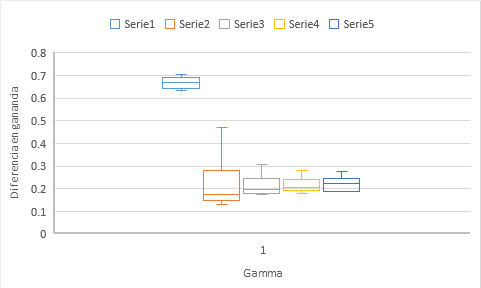
\includegraphics[scale=1]{Cajas1.png}
	\caption{Diagramas BoxPlot para la variable Gamma}
	\label{Cajas1}
\end{figure}

\begin{figure} [H]
	\centering
	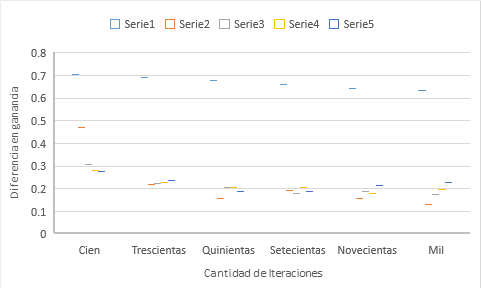
\includegraphics[scale=1]{Cajas1_1.png}
	\caption{Diagramas BoxPlot para la variable Iteraciones}
	\label{Cajas1_1}
\end{figure}

En estas figuras se ve la gran diferencia en los diagramas cuando se quiere observar media y varianza para cada valor, siendo razonable el resultado en los valores de gamma, donde lo que varía es el número de iteraciones, y tomadas como cinco valores aislados para cada valor en la cantidad de iteraciones, cuando la que variaba era gamma. Este comportamiento se debe a que al aumentar la cantidad de iteraciones en el experimento, se obtienen menores valores en la diferencia de las ganancias, mientras que al aumentar gamma, puede mejorar o empeorar el valor de la diferencia de las ganancias indistintamente.

Con los datos de la misma tabla \ref{experimento1}, se genera el análisis de varianza ANOVA, el cual se presta en la tabla \ref{tab:Anova1}. 

\begin{table}[H]
\centering\caption{ANOVA para Distancias en ganancias usando Gamma}
\small
\begin{tabular}{lrrrr}
\multicolumn{5}{c}{\textbf{ANÁLISIS DE VARIANZA}}             \\
\multicolumn{1}{c}{\textit{\textbf{\begin{tabular}[c]{@{}c@{}}Origen de las \\ \\ variaciones\end{tabular}}}} & \multicolumn{1}{c}{\textit{\textbf{\begin{tabular}[c]{@{}c@{}}Promedio de \\ \\ los cuadrados\end{tabular}}}} & \multicolumn{1}{c}{\textit{\textbf{F}}} & \multicolumn{1}{c}{\textit{\textbf{Probabilidad}}} & \multicolumn{1}{c}{\textit{\textbf{\begin{tabular}[c]{@{}c@{}}Valor crítico \\ \\ para F\end{tabular}}}} \\
                  & \multicolumn{1}{l}{}                                               & \multicolumn{1}{l}{}                    & \multicolumn{1}{l}{}                               & \multicolumn{1}{l}{}                                          \\
\textbf{Gamma}                                                                                                & 340127.902                                    & 16.7727717                              & 0.0000002762                                       & 2.602987403                                        \\
\textbf{Iteraciones}                                                                                             & 20273.7958                                       & 0.9997643429                            & 0.4382016733                                       & 2.602987403                                     
\end{tabular}
\label{tab:Anova1}
\end{table}

Para la primera variable, Gamma, se obtiene el valor de \textit{F} mayor al de \textit{F crítica} y una probabilidad muy baja $(P<0.05)$, lo que indica que existe una diferencia significativa en Gamma que afecta la variable dependiente.

Para la segunda variable, Iteraciones, se obtiene el valor de \textit{F} menor al de \textit{F crítica} y una probabilidad muy alta $(P>0.05)$, lo que indica que no existe una diferencia significativa en el número de iteraciones que afecta la variable dependiente.


\chapter{Resultados computacionales}
\label{resul_compu}

En este capítulo se presentan los resultados de los experimentos que se ejecutaron para ajustar algunos parámetros del algoritmo y para verificar el efecto de la aleatoriedad en el mismo. Para ello se toma el grafo de 5 etapas y 13 nodos con valores fijos para sus respectivos \textit{bandits}, los cuales tiene la característica que, en cada etapa, uno de ellos es suficientemente mejor que los demás y hará que, seguramente, tal nodo forme parte  del vector de acciones seleccionadas al final de las 5 etapas. 

Los valores que se fijaron para la matriz de adyacencia y para los valores reales de los \textit{bandits} del grafo que se usará en los experimentos descritas en este capítulo, son los siguientes:

\renewcommand{\arraystretch}{0.5}
%\begin{equation}
A = 
$\begin{bmatrix}
%\hspace{2cm}

0, 1, 1,  1,  0,  0,  0,  0,  0,  0,  0,  0,  0\\
0, 0, 0,  0,  0,  1,  1,  1,  1,  0,  0,  0,  0\\
0, 0, 0,  0,  1,  1,  0,  1,  1,  0,  0,  0,  0\\
0, 0, 0,  0,  0,  1,  1,  0,  0,  0,  0,  0,  0\\
0, 0, 0,  0,  0,  0,  0,  0,  0,  1,  0,  1,  0\\
0, 0, 0,  0,  0,  0,  0,  0,  0,  0,  0,  1,  0\\
0, 0, 0,  0,  0,  0,  0,  0,  0,  0,  1,  1,  0\\
0, 0, 0,  0,  0,  0,  0,  0,  0,  0,  0,  1,  0\\
0, 0, 0,  0,  0,  0,  0,  0,  0,  0,  1,  0,  0\\
0, 0, 0,  0,  0,  0,  0,  0,  0,  0,  0,  0,  1\\
0, 0, 0,  0,  0,  0,  0,  0,  0,  0,  0,  0,  1\\
0, 0, 0,  0,  0,  0,  0,  0,  0,  0,  0,  0,  1\\
0, 0, 0,  0,  0,  0,  0,  0,  0,  0,  0,  0,  0
\end{bmatrix}$

%\end{equation}

%\begin{figure}
%	\centering
%	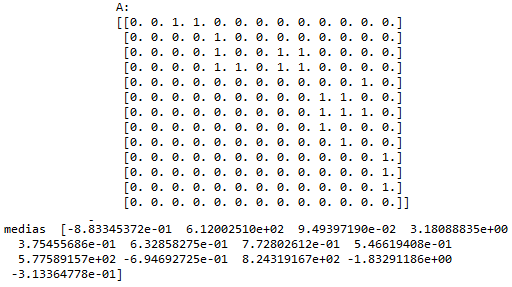
\includegraphics[scale=1]{MatrizAyBandits2}
%	\caption{Matriz y bandit generados}
%	\label{AyB}
%\end{figure}

$B$ = [2.29, 0.94, 193.06, -1.36, 190.22, -33.15, -0.42, -0.13, 2.46, 0.02, -0.81, 111.38, 1.38]

Es necesario tener en cuenta que aún se han dejando en forma aleatoria la selección inicial de los nodos y los valores distorsionados que se generan para los \textit{bandits} en cada iteración.

El grafo, con las aristas indicadas en la matriz de adyacencia y los valores de los \textit{bandits} del vector $B$, se aprecia en la figura \ref{Grafocaso1}
\begin{figure}[H]
	\centering
	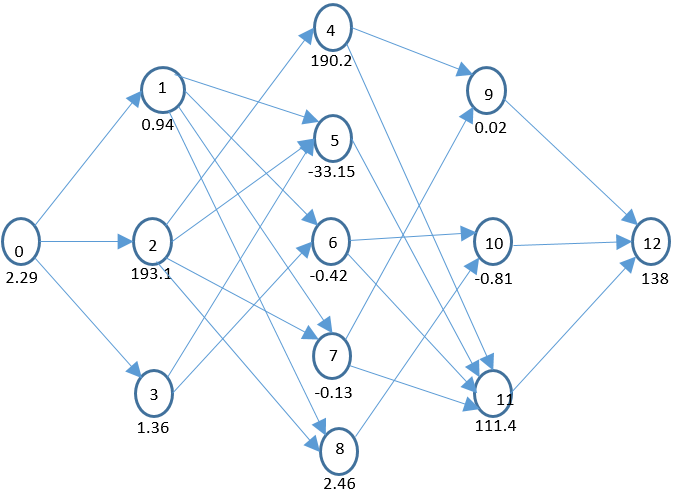
\includegraphics[scale=0.8]{Grafo5L.png}
	\caption{Grafo para las pruebas de parámetros}
	\label{Grafocaso1}
\end{figure}

\textit{Para estimar el desempeño del algoritmo se verificará la convergencia de los promedios de las ganancias distorsionadas hacia la ganancia real. Para facilitar la visualización de este comportamiento se hace una diferencia ente los valores de estas dos magnitudes, pero se normaliza para producir valores entre 0 y 1, con una sencilla división en el valor máximo posible, siendo el mejor valor el que más se acerque a la cero.}

\section{Parámetro Deltha puro}

Se retoman aquí las fórmulas con las que se consigue que el autómata aprenda y genere una matriz de probabilidades de transición entre nodos, para contextualizar el \textbf{parámetro de aprendizaje} $\delta$ que permite la actualización de una iteración a otra de la función de valor de los nodos, como se se muestra en la fórmula \ref{exponente4}.
\begin{eqnarray}\label{exponente4}
v_j(\tau + 1) = v_j(\tau) \pm \delta,
\end{eqnarray}

Estos valores son los exponentes que se usan en la fórmula de cálculo de probabilidades \ref{prob4}, que también se va actualizando para todos los pares de nodos en cada iteración.
\begin{eqnarray}\label{prob4}
P(i \to j) = \frac{e^{v_j}}{\sum_k A_{i,k} e^{v_k}},
\end{eqnarray}


\subsection{Prueba inicial}

Se realiza inicialmente una prueba con 9 valores para $\delta$ entre 0.1 y 0.9, sumando, en caso de ganancia y restando, en caso de pérdida, para motivar o desmotivar al autómata para que en el paso siguiente seleccione los nodos que reciben el refuerzo; la cantidad de iteraciones $T$ se varió entre 100 y 1000, con intervalos de 100. Las diferencias normalizadas que se encontraron entre la ganancia real y cada una de las ganancias que en promedio se obtuvieron se ven en la tabla \ref{tabla10}.

\begin{table}[h]
\small
\caption{Rangos de diferencia de ganancias con Deltha en décimas}
\begin{tabular}{crrrrrrrrrr}
\hline
\multicolumn{1}{l}{Deltha} & \multicolumn{10}{c}{Iteraciones} \\ \hline
\multicolumn{1}{l}{}       & \multicolumn{1}{c}{100} & \multicolumn{1}{c}{200} & \multicolumn{1}{c}{300} & \multicolumn{1}{c}{400} & \multicolumn{1}{c}{500} & \multicolumn{1}{c}{600} & \multicolumn{1}{c}{700} & \multicolumn{1}{c}{800} & \multicolumn{1}{c}{900} & \multicolumn{1}{c}{1000} \\ \hline
0,1                          & 0.715                    & 0.715                    & 0.715                    & 0.715                    & 0.715                    & 0.715                    & 0.715                    & 0.715                    & 0.715                    & 0.715                     \\ 
0,2                          & 0.695                    & 0.695                    & 0.695                    & 0.695                    & 0.695                    & 0.695                    & 0.695                    & 0.695                    & 0.695                    & 0.695                     \\ 
0,3                          & 0.676                    & 0.676                    & 0.676                    & 0.676                    & 0.676                    & 0.676                    & 0.676                    & 0.676                    & 0.676                    & 0.676                     \\ 
0,4                          & 0.656                    & 0.656                    & 0.656                    & 0.656                    & 0.656                    & 0.656                    & 0.656                    & 0.656                    & 0.656                    & 0.656                     \\ 
0,5                          & 0.637                    & 0.637                    & 0.637                    & 0.637                    & 0.637                    & 0.637                    & 0.637                    & 0.637                    & 0.637                    & 0.637                     \\ 
0,6                          & 0.618                    & 0.618                    & 0.618                    & 0.618                    & 0.618                    & 0.618                    & 0.618                    & 0.618                    & 0.618                    & 0.618                     \\ 
0,7                          & 0.598                    & 0.598                    & 0.598                    & 0.598                    & 0.598                    & 0.598                    & 0.598                    & 0.598                    & 0.598                    & 0.598                     \\ 
0,8                          & 0.579                    & 0.579                    & 0.579                    & 0.579                    & 0.579                    & 0.579                    & 0.579                    & 0.579                    & 0.579                    & 0.579                     \\ 
0,9                          & 0.559                    & 0.559                    & 0.559                    & 0.559                    & 0.559                    & 0.559                    & 0.559                    & 0.559                    & 0.559                    & 0.559                     \\ \hline
\end{tabular}
\label{tabla10}
\end{table}
Los rangos de diferencia superan el 50\%, independientemente de la cantidad de iteraciones que se ejecuten, por lo que se procede a experimentar con valores de $\delta$ de órdenes diferentes. 

\subsection{Segunda prueba}

Se ejecuta la aplicación con valores de $\delta$ en magnitudes de centésimas, milésimas y diezmilésimas y con los mismos 10 valores para la cantidad de iteraciones $T$, cuyos resultados se aprecian en la tabla \ref{tabla100_10000}.

\begin{table}[h]
\small

\caption{Rangos de diferencia de ganancias con Deltha en otras unidades}
\begin{tabular}{rrrrrrrrrrr} 
\multicolumn{1}{l}{Deltha} & \multicolumn{10}{c}{Iteraciones}      \\ \hline                                                                                                                                                                                              \\
\multicolumn{1}{l}{}       & 100                  & 200                  & 300                  & 400                  & 500                  & 600                  & 700                  & 800                  & 900                  & 1000                 \\
0.01                       & 0.697                & 0.697                & 0.671                & 0.695                & 0.675                & 0.677                & 0.661                & 0.694                & 0.654                & 0.692                \\
0.02                       & 0.707                & 0.686                & 0.628                & 0.583                & 0.565                & 0.605                & 0.661                & 0.751                & 0.760                & 0.809                \\
0.03                       & 0.615                & 0.698                & 0.763                & 0.744                & 0.742                & 0.734                & 0.777                & 0.512                & 0.813                & 0.819                \\
0.04                       & 0.646                & 0.651                & 0.533                & 0.783                & 0.812                & 0.800                & 0.505                & 0.495                & 0.815                & 0.820                \\
0.05                       & 0.816                & 0.720                & 0.780                & 0.795                & 0.504                & 0.484                & 0.483                & 0.798                & 0.817                & 0.492                \\
0.06                       & 0.607                & 0.475                & 0.806                & 0.555                & 0.809                & 0.537                & 0.459                & 0.817                & 0.819                & 0.476                \\
0.07                       & 0.725                & 0.764                & 0.774                & 0.810                & 0.824                & 0.514                & 0.824                & 0.831                & 0.837                & 0.822                \\
0.08                       & 0.654                & 0.806                & 0.450                & 0.472                & 0.492                & 0.476                & 0.490                & 0.421                & 0.471                & 0.466                \\
0.09                       & 0.756                & 0.765                & 0.502                & 0.604                & 0.486                & 0.820                & 0.780                & 0.775                & 0.827                & 0.835                \\ \hline
\multicolumn{1}{l}{}       & \multicolumn{1}{l}{} & \multicolumn{1}{l}{} & \multicolumn{1}{l}{} & \multicolumn{1}{l}{} & \multicolumn{1}{l}{} & \multicolumn{1}{l}{} & \multicolumn{1}{l}{} & \multicolumn{1}{l}{} & \multicolumn{1}{l}{} & \multicolumn{1}{l}{} \\
\multicolumn{1}{l}{Deltha} & \multicolumn{10}{c}{Iteraciones}   \\ \hline                                                                                                                                                                                                   \\
\multicolumn{1}{l}{}       & 100                  & 200                  & 300                  & 400                  & 500                  & 600                  & 700                  & 800                  & 900                  & 1000                 \\
0.001                      & 0.690                & 0.699                & 0.705                & 0.713                & 0.705                & 0.704                & 0.708                & 0.727                & 0.713                & 0.698                \\
0.002                      & 0.702                & 0.710                & 0.706                & 0.715                & 0.716                & 0.696                & 0.682                & 0.680                & 0.696                & 0.714                \\
0.003                      & 0.647                & 0.719                & 0.682                & 0.692                & 0.699                & 0.700                & 0.709                & 0.691                & 0.687                & 0.659                \\
0.004                      & 0.711                & 0.721                & 0.697                & 0.694                & 0.688                & 0.687                & 0.671                & 0.691                & 0.681                & 0.693                \\
0.005                      & 0.763                & 0.691                & 0.710                & 0.682                & 0.688                & 0.686                & 0.667                & 0.664                & 0.684                & 0.689                \\
0.006                      & 0.692                & 0.726                & 0.693                & 0.692                & 0.716                & 0.689                & 0.654                & 0.680                & 0.647                & 0.605                \\
0.007                      & 0.730                & 0.695                & 0.696                & 0.680                & 0.680                & 0.656                & 0.674                & 0.626                & 0.706                & 0.656                \\
0.008                      & 0.728                & 0.651                & 0.708                & 0.669                & 0.668                & 0.686                & 0.681                & 0.710                & 0.692                & 0.665                \\
0.009                      & 0.707                & 0.695                & 0.644                & 0.691                & 0.640                & 0.717                & 0.714                & 0.614                & 0.703                & 0.692                \\ \hline
\multicolumn{1}{l}{}       & \multicolumn{1}{l}{} & \multicolumn{1}{l}{} & \multicolumn{1}{l}{} & \multicolumn{1}{l}{} & \multicolumn{1}{l}{} & \multicolumn{1}{l}{} & \multicolumn{1}{l}{} & \multicolumn{1}{l}{} & \multicolumn{1}{l}{} & \multicolumn{1}{l}{} \\
\multicolumn{1}{l}{Deltha} & \multicolumn{10}{c}{Iteraciones}    \\ \hline                                                                                                                                                                                                  \\
\multicolumn{1}{l}{}       & 100                  & 200                  & 300                  & 400                  & 500                  & 600                  & 700                  & 800                  & 900                  & 1000                 \\
0.0001                     & 0.708                & 0.689                & 0.728                & 0.718                & 0.693                & 0.709                & 0.700                & 0.694                & 0.709                & 0.699                \\
0.0002                     & 0.684                & 0.697                & 0.718                & 0.696                & 0.710                & 0.734                & 0.700                & 0.706                & 0.708                & 0.699                \\
0.0003                     & 0.718                & 0.683                & 0.693                & 0.699                & 0.706                & 0.715                & 0.699                & 0.707                & 0.715                & 0.696                \\
0.0004                     & 0.748                & 0.717                & 0.704                & 0.707                & 0.710                & 0.745                & 0.705                & 0.705                & 0.707                & 0.713                \\
0.0005                     & 0.686                & 0.692                & 0.705                & 0.733                & 0.700                & 0.706                & 0.709                & 0.691                & 0.704                & 0.717                \\
0.0006                     & 0.649                & 0.742                & 0.703                & 0.711                & 0.699                & 0.685                & 0.717                & 0.706                & 0.707                & 0.706                \\
0.0007                     & 0.752                & 0.723                & 0.733                & 0.706                & 0.700                & 0.701                & 0.688                & 0.709                & 0.697                & 0.722                \\
0.0008                     & 0.682                & 0.725                & 0.704                & 0.706                & 0.720                & 0.690                & 0.700                & 0.712                & 0.705                & 0.709                \\
0.0009                     & 0.718                & 0.680                & 0.708                & 0.691                & 0.694                & 0.702                & 0.702                & 0.714                & 0.688                & 0.698          \\ \hline       
\end{tabular}
\label{tabla100_10000}
\end{table}

Aquí se puede apreciar que, a pesar de disminuir notablemente los valores de $\delta$, se siguen obteniendo valores muy altos para la diferencia de las ganancias, con errores superiores al 40\%. Los promedios de estas diferencias se presentan en la tabla \ref{delthas_0000}, donde además se aprecia que no hay una diferencia relevante para las diferentes magnitudes de $\delta$.

\begin{table}[h]
\centering
%\small
\caption{Promedios de los resultados variando décimas en Deltha}
\begin{tabular}{llll} \\ \hline  
\multicolumn{4}{c}{\textbf{PROMEDIOS DE ERROR EN GANANCIAS}}                                                  \\ \hline  
\textbf{Décimas}          & \textbf{Centésimas}       & \textbf{Milésimas}        & \textbf{Diezmilésimas}    \\ \hline  
\multicolumn{1}{r}{0.637} & \multicolumn{1}{r}{0.675} & \multicolumn{1}{r}{0.690} & \multicolumn{1}{r}{0.706} \\ \hline  
\end{tabular}
\label{delthas_0000}
\end{table}

Con estos resultados, se formulan experimentos con una mayor variación para $\delta$ y para la cantidad de Iteraciones $T$, que permita un análisis estadístico de la influencia de estas dos variables en los resultados esperados.

\subsection{Experimentos}

\subsubsection{Variable dependiente}

Se define como variable dependiente para este conjunto de experimentos a la diferencia entre la ganancia real máxima y la ganancia distorsionada media obtenida en la ejecución, normalizada de forma que se obtengan valores entre cero y uno. Se busca minimizar esta diferencia.

\subsubsection{Variables independientes}
Los experimentos se diseñan teniendo en cuenta que las variables independientes corresponden a: 
\begin{itemize}
    \item Factor de aprendizaje $\delta$
    \item Número de iteraciones $T$
\end{itemize}

\subsubsection{Validez}
Para el control o validez interna se ha de comprobar que las variables, aquí definidas como independientes, son las que realmente influyen en las dependientes, y no factores externos como la aleatoriedad. Se toman, entonces, los resultados de 100 experimentos con cada uno de los valores de control sobre las variables independientes.

\subsubsection{Técnica}
La técnica que se usa en este experimento es la simulación. Es un instrumento objetivo, confiable y válido. La validez es alta, puesto que el computador siempre tratará los valores de la misma manera; se espera que con un mismo valor de variables independientes se obtengan resultados similares en las variables dependientes.

\subsubsection{Herramientas}
Se realizan los cálculos de medias, varianzas y de análisis de varianza (ANOVA) que permitan concluir la forma en que cada variable independiente influye en la dependiente.

\subsubsection{Experimento uno}

Se diseña un experimento con las variables independientes: $T$ y $\delta$, correspondientes a la cantidad de iteraciones y al factor de aprendizaje que ha de incentivar la selección o no de un nodo, ya que afecta la matriz de probabilidades de transición; la variable dependiente corresponde a la diferencia normalizada de las ganancias, ya descrita.

%Se adiciona a la aplicación una variable que mide el porcentaje de veces que el vector final corresponde al esperado, la cual permite corroborar que las soluciones con diferencias de ganancia cercanas a cero, ofrecen, en una cantidad cercana al 100\%, el vector solución que se espera y que la convergencia de la ganancia obtenida, sí se está dando hacia la ganancia óptima.

Se usan valores para $T$ de 100, 1000, 10000 y 100000 iteraciones y valores de $\delta$ de $10^{2}$, $10^{1}$, $10^{0}$, $10^{-1}$, $10^{-2}$, $10^{-3}$ y $10^{-4}$. Este experimento se ejecuta varias veces, encontrando diferentes valores en sus resultados para los mismo valores de $T$ y de $\delta$, lo que se explica por la influencia de la aleatoriedad en estos resultados y se corrobora con el valor del estadístico de prueba $F$ y el valor de $P$ de las tablas ANOVA. Las gráficas correspondientes a tres ejecuciones de este experimento y los resultados del ANOVA correspondiente, se presentan en la tabla \ref{exp1}.
\begin{table}[H]
\caption{Experimento uno con Deltha}
\centering
\begin{tabular}[c]{llll}
\multicolumn{1}{p{2.9cm}}{\textbf{GRÁFICA PARA $\delta$}} & \multicolumn{1}{p{2.9cm}}{\textbf{GRÁFICA PARA $T$}} & \multicolumn{1}{p{2.9cm}}{\textbf{GRÁFICA PARA $T$ y $\delta$}} & \multicolumn{1}{p{2.9cm}}{\textbf{ANOVA}}  \\ \hline
\multicolumn{1}{|l|}{\includegraphics[align=t, width=33mm]{cajasDeltha_exp11.jpg}}    & \multicolumn{1}{l|}{\includegraphics[align=t, width=33mm]{cajasT1_exp11.jpg} } & \multicolumn{1}{l|}{\includegraphics[align=t, width=33mm]{cajasT_Deltha_exp11.jpg} } &
\multicolumn{1}{p{3cm}|}{\includegraphics[align=t, width=30mm]{Anova11.png}}     \\ \hline
\multicolumn{1}{|l|}{\includegraphics[align=t, width=33mm]{cajasDeltha_exp12.jpg}}    & \multicolumn{1}{l|}{\includegraphics[align=t, width=33mm]{cajasT1_exp12.jpg} } & \multicolumn{1}{l|}{\includegraphics[align=t, width=33mm]{cajasT_Deltha_exp12.jpg} } & \multicolumn{1}{p{3cm}|}{\includegraphics[align=t, width=30mm]{Anova12.png}} \\ \hline
\multicolumn{1}{|l|}{\includegraphics[align=t, width=33mm]{cajasDeltha_exp13.jpg}}    & \multicolumn{1}{l|}{\includegraphics[align=t, width=33mm]{cajasT1_exp13.jpg} } & \multicolumn{1}{l|}{\includegraphics[align=t, width=33mm]{cajasT_Deltha_exp13.jpg} } & \multicolumn{1}{p{3cm}|}{\includegraphics[align=t, width=30mm]{Anova13.png}} \\ \hline
\end{tabular}
\label{exp1}
\end{table}

En las tres filas de la tabla \ref{exp1} se notan cambios en las medias y las varianzas obtenidos de una ejecución a otra, y en las tablas ANOVA se puede verificar que la probabilidad $PR(>F)$ se mantuvo con valores superiores a 0.05, en casi todos los casos; en  pero en el tercer caso, para la variable $\delta$ sí se obtuvo un valor menor de 0.05 en dicha columna de probabilidad. Estos resultados no nos permiten concluir que las variables independientes tengan un alto grado de significancia sobre la variable dependiente; además, se esperaría que, en general, el estadístico de prueba $F$ tuviera siempre un valor distante de la unidad y los seis valores obtenidos son relativamente cercanos a la unidad. 

Además estas gráficas muestran que, independientemente de la cantidad de iteraciones que se hagan (variable $T$, eje horizontal), se obtienen resultados muy altos para la diferencia normalizada de ganancias, con medias que llegan a estar por encima del 70\%. Coincide en las tres ocasiones que la varianza en las cajas para el menor valor de $T$ es la más pequeña; esto se debe a que en estos casos, y especialmente cuando se tienen valores grandes para $\delta$, el algoritmo tiende a aprender una de las primeras respuestas que, aleatoriamente, debió validar y se queda con ella convergiendo rápidamente a cualquier respuesta, que no es necesariamente la óptima. Se procede entonces a verificar lo que sucede con valores grandes para $T$ y pequeños para $\delta$.

Se quiere observar si algunos de los valor de $T$ y de $delta$ que en la gráfica muestran mejores resultados, influyen efectivamente en la optimización de la diferencia entre ganancias.

\subsubsection{Experimento dos con Deltha}

%Se diseña un experimento con las mismas dos variables independientes: T y $\delta$, y la misma variable dependiente corresponde a la diferencia normalizada de las ganancias que debe corresponder con los resultados del porcentaje de veces que el vector final corresponde al esperado.

Se usan, en esta ocasión, valores para $T$ de 100000 y 100001 (se deja casi la misma cantidad, para estimar básicamente el comportamiento de la variable $\delta$) y valores de $delta$ de $10^{-3}$ y $10^{-4}$. Este experimento se ejecuta varias veces, encontrando diferentes valores en sus resultados para los mismos valores de $T$ y de $\delta$, lo que se explica como una alta influencia de la aleatoriedad. 

Tres resultados con los mismos valores de la variables independientes se muestran en la figura \ref{exp2}

\begin{table}[h]
\caption{Experimento dos}
\centering
\begin{tabular}[c]{llll}
\multicolumn{1}{p{2.9cm}}{\textbf{GRÁFICA PARA $\delta$}} & \multicolumn{1}{p{2.9cm}}{\textbf{GRÁFICA PARA $T$}} & \multicolumn{1}{p{2.9cm}}{\textbf{GRÁFICA PARA $T$ y $\delta$}} & \multicolumn{1}{p{2.9cm}}{\textbf{ANOVA}}  \\ \hline
\multicolumn{1}{|l|}{\includegraphics[align=t, width=33mm]{cajasDeltha_exp21.jpg}}    & \multicolumn{1}{l|}{\includegraphics[align=t, width=33mm]{cajasT1_exp21.jpg} } & \multicolumn{1}{l|}{\includegraphics[align=t, width=33mm]{cajasT_Deltha_exp21.jpg} } &
\multicolumn{1}{p{3cm}|}{\includegraphics[align=t, width=30mm]{Anova21.png}}     \\ \hline
\multicolumn{1}{|l|}{\includegraphics[align=t, width=33mm]{cajasDeltha_exp22.jpg}}    & \multicolumn{1}{l|}{\includegraphics[align=t, width=33mm]{cajasT1_exp22.jpg} } & \multicolumn{1}{l|}{\includegraphics[align=t, width=33mm]{cajasT_Deltha_exp22.jpg} } & \multicolumn{1}{p{3cm}|}{\includegraphics[align=t, width=30mm]{Anova22.png}} \\ \hline
\multicolumn{1}{|l|}{\includegraphics[align=t, width=33mm]{cajasDeltha_exp23.jpg}}    & \multicolumn{1}{l|}{\includegraphics[align=t, width=33mm]{cajasT1_exp23.jpg} } & \multicolumn{1}{l|}{\includegraphics[align=t, width=33mm]{cajasT_Deltha_exp23.jpg} } & \multicolumn{1}{p{3cm}|}{\includegraphics[align=t, width=30mm]{Anova23.png}} \\ \hline
\end{tabular}
\label{exp2}
\end{table}

Los resultados de las tablas ANOVA en la ejecución de la fila $1$ de la tabla \ref{exp2} presentan un valor para el estadístico de prueba $F$ mucho mayor que 1 y el valor de la probabilidad $PR(>F)$ menor a 0.05, para la variable $\delta$, lo que indicaría que esta variable independiente influye notoriamente en la variable dependiente; pero en las dos ejecuciones que se muestran al final de la tabla, no se mantuvo este resultado para $\delta$, obteniendo valores en $PR(>F)$ superiores a 0.05; así mismo para la variable $T$. Estos resultados no nos permiten, nuevamente, concluir que las variables independientes tengan un alto grado de significancia sobre la variable dependiente.

Se decide, entonces trabajar con una variable $\delta$ dependiente de la magnitud de la ganancia o pérdida que se reciba al final de cada ruta probada, como se explica en el siguiente experimento.

\section{Parámetro Gamma}

Se procede a cambiar $\delta$ por un valor que cambiará en función de la ganancia que se recibe al final de la ruta probada, de forma que, inclusive, el signo se ajustará cuando hayan pérdidas, sin hacerse necesario decidir entre suma y resta. Para ello se involucra un factor de aprendizaje Gamma ($\gamma$) que dosificará la retribución que tendrá la ganancia en el ajuste de la función de valor de los \textit{bandits} asociados a los nodos de la ruta probada, como se aprecia en la ecuación \ref{gama}, al multiplicar $\gamma$ por la ganancia ($Gain$) o recompensa recibida al final del camino.
\begin{eqnarray}
\label{gama}
v_j(\tau + 1) = v_j(\tau) + \gamma Gain
\end{eqnarray}

El valor de $\gamma$ ha de ser lo suficientemente pequeño para garantizar que, al multiplicarlo por la ganancia, la cantidad se reduzca a valores menores de 1 en su valor absoluto.

\subsection{Primer caso de estudio}

Inicialmente se realizó una prueba para establecer el porcentaje de ejecuciones en que el algoritmo realmente converge, ejecutando varias veces el algoritmo con el grafo ya fijo. En esta, se ha encontrado una tendencia a que solo en 7 de cada 10 ocasiones se logra la convergencia hacia el valor real. Las gráficas de la figura \ref{Ejecuta10} corresponden a 10 corridas del algoritmo de probabilidades aprendidas con 1000 iteraciones, un $\delta$ de aprendizaje que se obtuvo de multiplicar $\gamma = 0.0003$ por el valor de la ganancia o recompensa de la ruta utilizada.

\begin{figure} 
    \centering
    \begin{subfigure}[b]{0.38\textwidth}
        \includegraphics[width=\textwidth]{grafi1.jpg}
        %\caption{A gull}
        \label{fig:gull}
    \end{subfigure}
    \vspace{0.5 mm}
    ~ %add desired spacing between images, e. g. ~, \quad, \qquad, \hfill etc. 
      %(or a blank line to force the subfigure onto a new line)
    \begin{subfigure}[b]{0.38\textwidth}
        \includegraphics[width=\textwidth]{grafi2.jpg}
        %\caption{A tiger}
        \label{fig:tiger}
    \end{subfigure}
    ~ %add desired spacing between images, e. g. ~, \quad, \qquad, \hfill etc. 
    %(or a blank line to force the subfigure onto a new line)
    \begin{subfigure}[b]{0.38\textwidth}
        \includegraphics[width=\textwidth]{grafi3.jpg}
        %\caption{A mouse}
        \label{fig:mouse}
    \end{subfigure}
    \begin{subfigure}[b]{0.38\textwidth}
        \includegraphics[width=\textwidth]{grafi4.jpg}
        %\caption{A tiger}
        \label{fig:tiger}
    \end{subfigure}
        \begin{subfigure}[b]{0.38\textwidth}
        \includegraphics[width=\textwidth]{grafi5.jpg}
        %\caption{A gull}
        \label{fig:gull}
    \end{subfigure}
    ~ %add desired spacing between images, e. g. ~, \quad, \qquad, \hfill etc. 
      %(or a blank line to force the subfigure onto a new line)
    \begin{subfigure}[b]{0.38\textwidth}
        \includegraphics[width=\textwidth]{grafi6.jpg}
        %\caption{A tiger}
        \label{fig:tiger}
    \end{subfigure}
    ~ %add desired spacing between images, e. g. ~, \quad, \qquad, \hfill etc. 
    %(or a blank line to force the subfigure onto a new line)
    \begin{subfigure}[b]{0.38\textwidth}
        \includegraphics[width=\textwidth]{grafi7.jpg}
        %\caption{A mouse}
        \label{fig:mouse}
    \end{subfigure}
    \begin{subfigure}[b]{0.38\textwidth}
        \includegraphics[width=\textwidth]{grafi8.jpg}
        %\caption{A tiger}
        \label{fig:tiger}
    \end{subfigure}
    \begin{subfigure}[b]{0.38\textwidth}
        \includegraphics[width=\textwidth]{grafi9.jpg}
        %\caption{A mouse}
        \label{fig:mouse}
    \end{subfigure}
    \begin{subfigure}[b]{0.38\textwidth}
        \includegraphics[width=\textwidth]{grafi10.jpg}
        %\caption{A tiger}
        \label{fig:tiger}
    \end{subfigure}    
    \caption{Ejecución algoritmo Probabilidad Modelada}
    \label{Ejecuta10}
\end{figure}

El hecho de que no todas las ejecuciones con los mismos valores de entrada, presenten la misma convergencia, refleja la influencia que sigue presentando la aleatoriedad en este modelo, lo que no es muy deseable.

Dado que esta prueba se hizo con un único valor para $T$ y un único valor para $\gamma$, se procedió a explorar otros valores para dichas variables que puedan mejorar este porcentaje de éxito.

\subsection{Experimentos}

Al igual que para los experimento que hicieron con la variable $\delta$, se explican loe elementos en seguida.

\subsubsection{Variable dependiente}

Se define como variable dependiente para este conjunto de experimentos a la diferencia entre la ganancia real máxima y la ganancia distorsionada obtenida en la ejecución, diferencia que se normaliza, de forma que se obtengan valores entre cero y uno.

\subsubsection{Variables independientes}
Los experimentos se diseñan teniendo en cuenta que las variables independientes corresponden a: 
\begin{itemize}
    \item Coeficiente del factor de aprendizaje $\gamma$
    \item Número de iteraciones $T$
\end{itemize}

\subsubsection{Validez}
Para el control o validez interna se ha de comprobar que las variables, aquí definidas como independientes, son las que realmente influyen en la variable dependiente, y no factores externos como la aleatoriedad. Se toman, entonces, los resultados de 100 experimentos con cada uno de los valores de control sobre las variables independientes.

\subsubsection{Técnica}
La técnica que se usa en este experimento es la simulación. Es un instrumento objetivo, confiable y válido. La validez es alta, puesto que el computador siempre tratará los valores de la misma manera; se espera que con un mismo valor de variables independientes se obtengan resultados similares en las variables dependientes.

\subsubsection{Herramientas}
Se realizan los cálculos de medias, varianzas y de análisis de varianza (ANOVA) que permitan concluir la forma en que cada variable independiente influye en la dependiente.

\subsubsection{Experimento uno}

Se asignan valores a las variables dependientes así: $T$ toma valores de 100, 300, 500, 700, 900 y 1000; y $\gamma$ valores de 0.00001, 0.00025, 0.00049, 0.00075, 0.0001, con los que se pretende cubrir los valores de $\gamma$ del orden de $10^{-4}$.

Los valores de los promedios en la diferencia de las ganancias que se obtuvieron se aprecian en la tabla \ref{experimento1}.

\begin{table}[H]
\centering
%\small
\caption{Promedios de diferencias de ganancias usando Gamma}
\begin{tabular}{cllllll}
%\multicolumn{7}{c}{DISTANCIAS EN GANANCIAS PROMEDIO}                                                                                   %                                            \\
GAMA                 & \multicolumn{6}{c}{ITERACIONES}    \\ \hline
\multicolumn{1}{l}{} & \multicolumn{1}{c}{100} & \multicolumn{1}{c}{300} & \multicolumn{1}{c}{500} & \multicolumn{1}{c}{700} & \multicolumn{1}{c}{900} & \multicolumn{1}{c}{1000} \\ \hline
0,00001              & 0,368                   & 0,360                    & 0,344                   & 0,328                   & 0,322                   & 0,272                    \\
0,00025              & 0,102                   & 0,044                   & 0,034                   & 0,066                   & 0,052                   & 0,042                    \\
0,00050              & 0,050                    & 0,078                   & 0,082                   & 0,072                   & 0,082                   & 0,074                    \\
0,00075              & 0,080                    & 0,092                   & 0,086                   & 0,090                    & 0,078                   & 0,090                     \\
0,00099              & 0,092                   & 0,102                   & 0,084                   & 0,084                   & 0,100                     & 0,106         \\ \hline
\end{tabular}
\label{experimento1}
\end{table}

Los resultados son considerablemente mejores que los que se obtuvieron con $\delta$, obteniendo un promedio en el error para esta tabla del 13\% (o del 8\%, si se elimina la primera fila donde se encuentran los valores más altos). También, se puede notar, en esta tabla, que los errores están influidos tanto por el valor de $\gamma$, como por el número de iteraciones que se ejecutan.

Utilizando los datos de la tabla \ref{experimento1}, se obtienen promedios y varianza para cada fila y para cada columna, como se presenta en la tabla \ref{media_var_1}.

\begin{table}[h]
\centering
%\small
\caption{Medias y varianzas en Promedios de distancias usando Gamma}
\begin{tabular}{rrr}
\multicolumn{1}{l}{}            & \multicolumn{1}{c}{\textit{\textbf{PROMEDIO}}} & \multicolumn{1}{c}{\textit{\textbf{VARIANZA}}} \\ \hline
\multicolumn{1}{l}{GAMMA}     & \multicolumn{1}{l}{}                           & \multicolumn{1}{l}{}                           \\
0.00001                         & 0.3323                                         & 0.001188                                       \\
0.00025                         & 0.0567                                         & 0.000611                                       \\
0.00050                         & 0.0730                                         & 0.000144                                       \\
0.00075                         & 0.0860                                         & 0.000034                                       \\
0.00099                         & 0.0947                                         & 0.000089                                       \\
\multicolumn{1}{l}{ITERACIONES}  & \multicolumn{1}{l}{}                           & \multicolumn{1}{l}{}                           \\
100                             & 0.1384                                         & 0.016855                                       \\
300                             & 0.1352                                         & 0.016273                                       \\
500                             & 0.126                                          & 0.015322                                       \\
700                             & 0.128                                          & 0.012590                                       \\
900                             & 0.1268                                         & 0.012201                                       \\
1000                            & 0.1168                                         & 0.008087 \\ \hline                                   
\end{tabular}
\label{media_var_1}
\end{table}

Aquí se puede notar que el valor de $\gamma$, no afecta significativamente las diferencias entre ganancias, mientras que cada vez que se aumentó el número de iteraciones $T$ en el experimento, los cambios fueron menores en la variable dependiente, lo que se apoya con el análisis de los resultados de las varianzas.

Se obtienen valores de varianzas pequeños, lo que es deseable al momento de tomar conclusiones sobre las medias dadas.

Este comportamiento se puede visualizar en los diagramas BoxPlot para Gamma y para el número de iteraciones que se ven en las figuras \ref{Cajas1} y \ref{Cajas1_1}, donde se aprecia, además que el incremento o decremento en los valores de gamma, no influye directamente en la diferencia entre ganancias mientras que el aumento en el número de iteraciones va disminuyendo, en general, dicha diferencia, aunque sea en cantidades muy pequeñas.


\begin{figure} [h]
	\centering
	\includegraphics[scale=1]{Cajas1.png}
	\caption{Diagramas BoxPlot para la variable Gamma}
	\label{Cajas1}
\end{figure}

\begin{figure} 
	\centering
	\includegraphics[scale=1]{Cajas1_1.png}
	\caption{Diagramas BoxPlot para la variable Iteraciones}
	\label{Cajas1_1}
\end{figure}


Para corroborar esta observación se genera el análisis de varianza ANOVA para los datos de la tabla \ref{experimento1}, cuyo resultado se presenta en la tabla \ref{tab:Anova1}. 

\begin{table} [h]
\centering\caption{ANOVA para Distancias en ganancias usando Gamma}
\small
\begin{tabular}{lrrrr} \\ 
%\multicolumn{5}{c}{\textbf{ANÁLISIS DE VARIANZA}}             \\
\multicolumn{1}{c}{\textit{\textbf{\begin{tabular}[c]{@{}c@{}}Origen de las \\ \\ variaciones\end{tabular}}}} & \multicolumn{1}{c}{\textit{\textbf{\begin{tabular}[c]{@{}c@{}}Promedio de \\ \\ los cuadrados\end{tabular}}}} & \multicolumn{1}{c}{\textit{\textbf{F}}} & \multicolumn{1}{c}{\textit{\textbf{Probabilidad}}} & \multicolumn{1}{c}{\textit{\textbf{\begin{tabular}[c]{@{}c@{}}Valor crítico \\ \\ para F\end{tabular}}}} \\ \hline
                  & \multicolumn{1}{l}{}                                               & \multicolumn{1}{l}{}                    & \multicolumn{1}{l}{}                               & \multicolumn{1}{l}{}                                          \\
\textbf{Gamma}                                                                                                & 0.244513                                    & 118.074                              & 1.297E-13                                       & 2.86608                                        \\ 
\textbf{Iteraciones}                                                                                             & 0.013214                                       & 6.381                            & 0.00107                                       & 2.71089         \\ \hline                            
\end{tabular}
\label{tab:Anova1}
\end{table}

Para la primera variable, $Gamma$, se obtiene el valor de \textit{F} mayor al de \textit{F crítica} y una probabilidad muy baja $(P<0.05)$, lo que indica que existe una diferencia significativa en Gamma que afecta la variable dependiente.

Para la segunda variable, $Iteraciones$, se obtiene el valor de \textit{F} mayor al de \textit{F crítica} y una probabilidad baja $(P<0.05)$, lo que indica que también existe una diferencia significativa en el número de iteraciones que afecta la variable dependiente, pero no de la misma forma que la variable $Gamma$, tal como se había planteado al analizar las gráficas BoxPlot.

Se quiere entonces, encontrar un valor de Gamma que ofrezca buenos resultados, y estimar hasta donde la cantidad de iteraciones puede disminuir considerablemente el valor de la variable dependiente, que corresponde a la diferencia entre las ganancias obtenidas y la ganancia real, para lo que se plantean los experimentos siguientes.

\subsubsection{Experimento dos}

%Se diseña un experimento con dos variables independientes: T y $\gamma$, correspondientes a la cantidad de iteraciones y a la variable que, multiplicada por la ganancia total asociada a la secuencia de nodos que se haya probado, como parámetro de aprendizaje. Se recuerda que la variable dependiente corresponde a la diferencia normalizada de las ganancias y que también se calcula el porcentaje de veces que el vector final corresponde al esperado cuyo valor debe estar cercano al 100\%, cuando el de la diferencia de ganancia se acerque al 0\%.

Para este experimento se usan valores para T de 100, 1000, 10000 y 100000 iteraciones y valores de $\gamma$ de $10^{0}$, $10^{-1}$, $10^{-2}$, $10^{-3}$, $10^{-4}$, $10^{-5}$, $10^{-6}$. Al ejecutar este experimento varias veces, se encuentra que los valores de sus resultados para los mismo valores de T y de $\gamma$, tienen tendencias marcadas, lo que permite establecer que la influencia de la aleatoriedad en estos resultados es menor que la que se observó en los experimentos anteriores. 

\begin{table}[H]
\caption{ANOVA para el Experimento dos con Gamma}
\centering
\begin{tabular}[c]{llll}
\multicolumn{1}{p{2.9cm}}{\textbf{GRÁFICA PARA $\gamma$}} & \multicolumn{1}{p{2.9cm}}{\textbf{GRÁFICA PARA $T$}} & \multicolumn{1}{p{2.9cm}}{\textbf{GRÁFICA PARA $T$ y $\gamma$}} & \multicolumn{1}{p{2.9cm}}{\textbf{ANOVA}}  \\ \hline
\multicolumn{1}{|l|}{\includegraphics[align=t, width=33mm]{cajasGamma_exp31.jpg}}    & \multicolumn{1}{l|}{\includegraphics[align=t, width=33mm]{cajasT_exp31.jpg} } & \multicolumn{1}{l|}{\includegraphics[align=t, width=33mm]{cajasT_Gamma_exp31.jpg} } &
\multicolumn{1}{p{3cm}|}{\includegraphics[align=t, width=30mm]{Anova31.png}}     \\ \hline
\multicolumn{1}{|l|}{\includegraphics[align=t, width=33mm]{cajasGamma_exp32.jpg}}    & \multicolumn{1}{l|}{\includegraphics[align=t, width=33mm]{cajasT_exp32.jpg} } & \multicolumn{1}{l|}{\includegraphics[align=t, width=33mm]{cajasT_Gamma_exp32.jpg} } & \multicolumn{1}{p{3cm}|}{\includegraphics[align=t, width=30mm]{Anova32.png}} \\ \hline
\multicolumn{1}{|l|}{\includegraphics[align=t, width=33mm]{cajasGamma_exp33.jpg}}    & \multicolumn{1}{l|}{\includegraphics[align=t, width=33mm]{cajasT_exp33.jpg} } & \multicolumn{1}{l|}{\includegraphics[align=t, width=33mm]{cajasT_Gamma_exp33.jpg} } & \multicolumn{1}{p{3cm}|}{\includegraphics[align=t, width=30mm]{Anova33.png}} \\ \hline
\end{tabular}
\label{exp3}
\end{table}

Tres de estos resultados se pueden ver en la tabla \ref{exp3}, donde, aunque el valor del estadístico de prueba $F$ de las tablas ANOVA aún no presenta valores lejanos a la unidad, el ejemplo de la segunda fila muestra valores para $PR(>F)$ menores a 0.05, para ambas variables. 
 
Estos cambios, que se ocasionan por la influencia de la aleatoriedad que aún se presenta, no permiten, una vez más, concluir que los valores de alguna de estas variables independientes influye efectivamente en los de la variable dependiente. 
 
Aún así, en las gráficas de la tabla \ref{exp3} se observa que se obtienen resultados de la diferencia normalizada de ganancias con medias que están por debajo del 80\% y que llegan a tomar valores cercanos al 0\%, especialmente con los valores más altos de la variable $T$ y más bajos para la variable $\gamma$. Lo anterior sugiere que con pequeños pasos y mayor cantidad de ellos, se puede llegar a obtener mejores resultados, lo que se verifica en el siguiente experimento.

\subsubsection{Experimento tres}

%Se diseña un experimento con las dos variables independientes: T y $\gamma$, correspondientes a la cantidad de iteraciones y a la variable que, multiplicada por la ganancia total asociada a la secuencia de nodos que se haya probado, como parámetro de aprendizaje. Se maneja la misma variable dependiente, corresponde a la diferencia normalizada de las ganancias como en los experimentos previos.

Para este experimento se usan valores para $T$ de 10000 a 100000 iteraciones con intervalos de 10000 y valores de $\gamma$ del orden de $10^{-4}$, teniendo en cuenta que fue la cifra que mostró los valores más bajos para la variable dependiente. 

Las gráficas correspondientes a tres ejecuciones de este experimento con sus gráficas y resultados del ANOVA, se presentan en la tabla \ref{exp4}.

\begin{table}[h]
\caption{ANOVA para el Experimento tres con Gamma}
\centering
\begin{tabular}[c]{llll}
\multicolumn{1}{p{2.95cm}}{\textbf{GRÁFICA PARA $\gamma$}} & \multicolumn{1}{p{2.95cm}}{\textbf{GRÁFICA PARA $T$}} & \multicolumn{1}{p{2.95cm}}{\textbf{GRÁFICA PARA $T$ y $\gamma$}} & \multicolumn{1}{p{2.95cm}}{\textbf{ANOVA}}  \\ \hline
\multicolumn{1}{|l|}{\includegraphics[align=t, width=33mm]{cajasGamma_exp4.jpg}}    & \multicolumn{1}{l|}{\includegraphics[align=t, width=33mm]{cajasT_exp4.jpg} } & \multicolumn{1}{l|}{\includegraphics[align=t, width=33mm]{cajasT_Gamma_exp4.jpg} } &
\multicolumn{1}{p{3.2cm}|}{\includegraphics[align=t, width=30mm]{Anova4.png}}     \\ \hline
\multicolumn{1}{|l|}{\includegraphics[align=t, width=33mm]{cajasGamma_exp42.jpg}}    & \multicolumn{1}{l|}{\includegraphics[align=t, width=33mm]{cajasT_exp42.jpg} } & \multicolumn{1}{l|}{\includegraphics[align=t, width=33mm]{cajasT_Gamma_exp42.jpg} } & \multicolumn{1}{p{3.2cm}|}{\includegraphics[align=t, width=30mm]{Anova42.png}} \\ \hline
\multicolumn{1}{|l|}{\includegraphics[align=t, width=33mm]{cajasGamma_exp43.jpg}}    & \multicolumn{1}{l|}{\includegraphics[align=t, width=33mm]{cajasT_exp43.jpg} } & \multicolumn{1}{l|}{\includegraphics[align=t, width=33mm]{cajasT_Gamma_exp43.jpg} } & \multicolumn{1}{p{3.2cm}|}{\includegraphics[align=t, width=30mm]{Anova43.png}} \\ \hline
\end{tabular}
\label{exp4}
\end{table}

Aunque las gráficas generadas al ejecutar este experimento varias veces, con los mismo valores de $T$ y de $\gamma$, parecen diferentes, mantienen valores para la variable independiente muy cercanos a cero, con valores inferiores al 2\% para todos los casos probados, lo que permite establecer una baja influencia de la aleatoriedad.

Los  valores del estadístico de prueba $F$ y de $PR(>F)$ de las tablas ANOVA muestran que no hay una dependencia entre los valores de la variable $\gamma$ y los resultados de la variable dependiente, puesto que $F$ toma valores cercanos a 1 y, $PR(>F)$ es mayor a 0.05. 

La independencia aparente de la variable $\gamma$ con los valores que toma la variable dependiente (diferencia promedio de ganancias distorsionadas) resulta ser un aspecto deseable para el experimento, puesto que los dos valores tomados para $\gamma$ solo difieren en $1*10^{-5}$, como se aprecia más claramente en la figura \ref{CajasGamma}, porque lo esperado era obtener resultados similares. 

\begin{figure}[H]
	\centering
	\includegraphics[scale=0.5]{cajasGamma_exp4.jpg}
	\caption{Diferencia normalizada de ganancias para $T$ y $\gamma$}
	\label{CajasGamma}
\end{figure}

De otra parte, en dos de los tres casos hay influencia de los valores que se dan a la variable $T$ sobre los obtenidos en la variable dependiente, ya que el valor de la probabilidad $PR(>F)$ es menor que 0.05; aspecto que resulta positivo para el modelo, porque lo acercan a un control inicial de los efectos de la aleatoriedad.

De aquí que, con cualquier valor de $T$ superior a 50000 iteraciones se obtuvieron excelentes resultados, con medias en la diferencias promedio de ganancias inferiores a 0.003 y varianzas muy pequeñas. Se elige entonces el valor de 100000 para la variable $T$ y de $10^{-4}$ para la variable $\gamma$, para generar el histograma en el que se apreciará cómo, efectivamente, la mayor parte de los valores de la variable dependiente se acerca a cero. Dicho histograma se muestra en la figura \ref{histo4}.

\begin{figure}[h]
	\centering
	\includegraphics[scale=0.5]{Histograma_gamma3.jpg}
	\caption{Diferencia normalizada a la ganancia real}
	\label{histo4}
\end{figure}

Vale aclarar que esta ejecución se realizó varias veces, encontrando siempre resultados similares, por lo que no se hace ningún comparativo adicional, sino que  se concluye que los valores probados en este experimento arrojan el resultado correcto.

Teniendo establecidos los parámetros de número de iteraciones y del factor de aprendizaje $\gamma$, se procede a probar el desempeño del algoritmo con grafos generados de forma aleatoria.

\section{Generación de un grafo aleatorio}

De acuerdo al diseño explicado en la sección \ref{algoritmos}, se ejecutó el programa de forma que aceptara como datos de entrada, además de los ya implementados, la cantidad de etapas del grafo y la cantidad de nodos en cada etapa. La generación de la matriz de adyacencia ha previsto para que cada nodo tenga al menos un nodo adyacente de la siguiente etapa, excepto si es de la ultima etapa, así como una densidad de conectividad entre los nodos del 66.67\%. 

Los valores de los \textit{bandits} se generan también de forma aleatoria con media en cero y desviación estándar de una unidad, pero se modifican computacionalmente para que uno de los nodos de cada etapa, elegido al azar, tenga asociada una ganancia positiva superior a la de los demás nodos de su etapa. 

Los valores generados para los \textit{bandits} se ajustaron para que las ganancias promedio quedaran del orden de las centenas, como las del grafo de prueba, ya que el valor de $\gamma$ depende de la magnitud de la ganancia que se obtenga en cada iteración.

El programa arroja resultados favorables con cantidad de etapas $L$ entre 5 y 12, observados en la convergencia del promedio de sus ganancias hacia la mayor ganancia real, dentro de los caminos probados por el algoritmo, como la que se aprecia en la figura \ref{Gangraforandom}. Uno de los casos se verifica manualmente, obteniendo el grafo a partir de la matriz de adyacencia generada aleatoriamente y de los valores generados para sus \textit{bandits}, con un valor para $L$ de 9 etapas y los siguientes valores para la cantidad de nodos por etapa: [1. 3. 4. 4. 3. 1.].

La gráfica se muestra en la figura \ref{graforandom} y su matriz de adyacencia es la siguiente:

\renewcommand{\arraystretch}{0.5}
%\begin{equation}
A = 
$\begin{bmatrix}
%\hspace{2cm}

0, 0, 1, 1,  0,  0,  0,  0,  0,  0,  0, 0, 0, 0, 0, 0\\
0, 0, 0, 0,  1,  1,  1,  0,  0,  0,  0, 0, 0, 0, 0, 0\\
0, 0, 0, 0,  0,  1,  0,  0,  0,  0,  0, 0, 0, 0, 0, 0\\
0, 0, 0, 0,  1,  0,  1,  1,  0,  0,  0, 0, 0, 0, 0, 0\\
0, 0, 0, 0,  0,  0,  0,  0,  1,  1,  1, 0, 0, 0, 0, 0\\
0, 0, 0, 0,  0,  0,  0,  0,  0,  0,  1, 1, 0, 0, 0, 0\\
0, 0, 0, 0,  0,  0,  0,  0,  1,  1,  0, 1, 0, 0, 0, 0\\
0, 0, 0, 0,  0,  0,  0,  0,  0,  1,  1, 0, 0, 0, 0, 0\\
0, 0, 0, 0,  0,  0,  0,  0,  0,  0,  0, 0, 1, 0, 1, 0\\
0, 0, 0, 0,  0,  0,  0,  0,  0,  0,  0, 0, 0, 1, 0, 0\\
0, 0, 0, 0,  0,  0,  0,  0,  0,  0,  0, 0, 1, 1, 1, 0\\
0, 0, 0, 0,  0,  0,  0,  0,  0,  0,  0, 0, 1, 1, 1, 0\\
0, 0, 0, 0,  0,  0,  0,  0,  0,  0,  0, 0, 0, 0, 0, 1\\
0, 0, 0, 0,  0,  0,  0,  0,  0,  0,  0, 0, 0, 0, 0, 1\\
0, 0, 0, 0,  0,  0,  0,  0,  0,  0,  0, 0, 0, 0, 0, 1\\
0, 0, 0, 0,  0,  0,  0,  0,  0,  0,  0, 0, 0, 0, 0, 0
\end{bmatrix}$

Así mismo el vector de \textit{bandits} generado de forma aleatoria fue el siguiente:

$B$ = [196.02255721, 9.32455363, 47.72564534, 66.21935444, 275.7996602, 6.62172573, 190.49629308, 13.33418851, 210.36419278, 37.39029137, 191.40773576, 117.1717095, 40.02228911, 220.45436046, 32.32878409, -125.16559689]

\begin{figure}[h]
	\centering
	\includegraphics[scale=0.4]{GrafoRandom.png}
	\caption{Grafo generado en forma aleatoria}
	\label{graforandom}
\end{figure}

\subsection{Prueba}

Se recuerda que las variables independientes son: la cantidad de Iteraciones $T$ y el factor de aprendizaje $\gamma$. El valor asignado al parámetro de $T$ es de 80000 iteraciones y el de $\gamma$ es de 0.000003. 

De otra parte, en esta prueba, además de la variable dependiente que se ha manejado en los experimentos anteriores, que ha sido el promedio de diferencias de ganancias normalizadas, se adiciona un indicador de salida que cuenta las veces que el vector solución generado por la aplicación corresponde con el vector óptimo.

Se mantiene la funcionalidad de la aplicación para establecer los valores óptimos del vector solución y de su ganancia real asociada, los que se obtienen guardando el valor de la ganancia real máxima que se vaya generando y su argumento (es decir el vector objeto de dicha ganancia).

Luego de la 80000 iteraciones con los parámetros ya explicados se obtuvieron las siguientes salidas:

\begin{itemize}
\item Promedio de la diferencia entre las ganancias obtenidas en cada iteración y la ganancia óptima: 0.019839554951030753, que es un valor inferior al 2\%.
\item Porcentaje de aciertos entre los vectores generados en cada iteración y el vector óptimo: 0.9531375, valor que supera el 95\% de coincidencias.
\item Vector óptimo = [0, 3, 4, 10, 13, 15], que corresponde al calculado del grafo de forma manual.
\end{itemize}

Además se generó la gráfica de convergencia de la ganancia que se obtienen en cada iteración y el resultado se muestra en la figura \ref{Gangraforandom}. En esta figura el eje horizontal corresponde al número de la iteración y el eje vertical a la ganancia obtenida en cada iteración.

\begin{figure}[h]
	\centering
	\includegraphics[scale=0.64]{GanGrafoRandom.png}
	\caption{Convergencia de ganancia con un grafo generado en forma aleatoria}
	\label{Gangraforandom}
\end{figure}

Es importante aclarar que, no se espera que el promedio de diferencias entre ganancias llegue a ser cero ni que el porcentaje de aciertos del vector generado con el vector óptimo llegue a ser uno, puesto que el autómata toma un tiempo en aprender la ruta óptima y solo se tendrán en cuenta los valores que el autómata haya tenido que probar durante las iteraciones. 

Finalmente se resalta el hecho de que la gráfica se estabiliza después de solo 10000 iteraciones, pero es necesario ejecutar cerca de 100000 para obtener resultados aceptable en el promedio normalizado de diferencias entre ganancias y en el porcentaje de aciertos con el vector óptimo; conseguir un criterio de parada para el algoritmo que disminuya el número de iteraciones será parte de la continuidad de esta investigación.
\chapter{Propuesta para CMMN}
\label{aplica}

Se retoma aquí el grafo que se genera al modelar un Caso con la notación CMMN. De tal esquema surge esta propuesta. La figura \ref{CMMN_modelo} presentada antes será la base para este ejemplo. 

\begin{figure}[h]
  \centering
    \includegraphics[scale=0.25]{ModeloCMM.png}
  \caption[Modelo CMMN]{Grafo en CMMMN que se llevará al modelo propuesto}
  \label{CMMN_modelo}
\end{figure}


\section{Modelo CMMN en un grafo por etapas}

Es importante recordar que las líneas punteadas de la figura \ref{CMMN_modelo} representan que la secuencia que se puede seguir o la presencia de algunas actividades es posible, pero no determinista.

Se vislumbra entonces, cómo esta notación CMMN puede llevarse al grafo con etapas propuesto, donde se pueda modelar la incertidumbre presente en la selección de tareas, disponiendo en cada etapa el conjunto de actividades posibles, para que el algoritmo de aprendizaje recomiende la tarea a seguir de la siguiente etapa.

Para esto se propone:

\begin{itemize}
    \item Si dostareas b y c están después de una tarea a, pero b y c no son disjuntas, entonces se deben ofrecer b y c en cualquiera de las etapas siguientes.
    \item Colocar una actividad nula en cada etapa para cuando no se ha de tomar alguna.
    \item Dejar las aristas suficientes para las posibles conexiones entre nodos, sin ocuparse demasiado por los prerrequisito, puesto que el algoritmo ha de aprender cuando los caminos no sean viables.
\end{itemize}


La figura \ref{CMMN_modelo} representa las tareas para escribir un artículo. En ella se pueden diferenciar claramente dos partes concernientes a la preparación del borrado y a su revisión. Estas partes permiten separar en dos figuras el grafo resultante de la propuesta de esta tesis.

Los grafos que se generaron a partir de esas apreciaciones se presentan en las figuras \ref{CMMN_modelo1} y \ref{CMMN_modelo2}.

\begin{figure}[h]
  \centering
    \includegraphics[scale=0.5]{DeCMMN1.jpg}
  \caption{Caso en etapas. Parte 1.}
  \label{CMMN_modelo1}
\end{figure}


\begin{figure}[h]
  \centering
    \includegraphics[scale=0.55]{DeCMMN2.jpg}
  \caption{Caso en etapas. Parte 2.}
  \label{CMMN_modelo2}
\end{figure}


También se ha considerado, para cuando se hace necesario traer de alguna forma la información pasada de actividades pasadas, que son predecesoras de otras, mediante la activación de una bandera que lo indique. Así mismo se analizó la posibilidad de fusionar actividades no disyuntas en un nodo ficticio, con la salvedad de que no es fácil esclarecer con certeza sus prerrequisitos.
%Un caso específico se presenta en el apéndice \ref{apendicecaso}, el cual se constituye como una parte del trabajo de investigación en el manejo de casos dinámicos de las BPMS que concibió el ingeniero Luis Chaparro, al interior del grupo de investigación GIPROCAS de la Universidad de Boyacá en Colombia.

%Dada esta introducción al caso de estudio, se procede a presentar las consultas bibliográficas correspondientes para establecer si el grafo propuesto ya se encuentra en otra investigación y si ya ha sido abordado un modelo cercano al \textit{L-n-armed-bandits}.
\chapter{Conclusiones y trabajo futuro}
Con esta tesis se presenta a la comunidad científica un modelo no reportado con una estructura de aprendizaje por refuerzo para problemas específicos por etapas de estado y tiempo finitos, dispuestos en un grafo por etapas que aprovecha estructura, para aprender de forma eficiente ua trayectoria óptima que de be seguir un agente.

Es una estructura sencilla, un modelo de decisión de Markov. 

Se inscribe dentro del campo de Aprendizaje por refuerzo para sistemas de decisión de Markov de estado finito y tiempo discreto (por episodios) y el número de tiempos en cada episodio también es finito.

Está estructurado en un grafo dirigido de principio a fin y esa estructura simple permite hacer un muestre eficiente para descubrir las trayectorias óptimas que debe seguir el agente.

La contribución básica teórica de ester trabajo es el encontrar una estructura sencilla de un proceso de decisión de Mrkov que estamos aprovechando para muestrear de modo eficiente.

Es una particularización de un problema muy general de Aprendizaje por refuerzo o de problemas de decisión de Markov que se resuelven mediante muestreo de Boltzman (Caso especial: aprovechar la estructura del Grafo por etapas)-> contribución a nivel metodológico y teórico. 

Una de las aplicaciones que se prevé para el modelo propuesto es el manejo de casos dinámicos por parte de las BPMS, dado que, siguiendo la notación CMMN, el caso se deja modelar con un grafo, el cual es susceptible de adaptar al grafo por etapas que se presenta en esta tesis, siguiendo las recomendaciones consignadas en el capítulo \ref{aplica}.

Muchos son los modelos de grafos que se han adecuado para la solución de problemas específicos y para los que se han creado algoritmos, con sus posteriores mejoras y adaptaciones. El modelo de grafo por etapas con nodos disjuntos de etapa a  etapa, no se encontró en la revisión de literatura que se hizo y se constituye en una alternativa para el modelado de problemas de decisión con alta incertidumbre, donde el efecto de la selección de cada nodo, solo se conoce al seleccionar el nodo de la última etapa.

El modelo de aprendizaje de probabilidades de transición entre nodos tiene bases matemáticas y maneja como parámetros la cantidad de tiempos de ejecución y el valor de un factor de aprendizaje $\delta$. La investigación arrojó que tal factor debe depender del signo y la magnitud de la ganancia que se obtenga en cada iteración, por lo que finalmente se manejó un coeficiente para dicho factor, que se denota como $\gamma$.

Para un grafo sencillo de etapas y 13 nodos con \textit{bandits} asociados del orden de las centenas, se concluyó que con 80000 tiempos y un coeficiente para el factor de aprendizaje del orden de 10e-4, se obtiene una convergencia aceptable hacia la ruta óptima. Al realizar experimentos con grafos de mayor dimensión, fue necesario ajustar el coeficiente del factor de aprendizaje con cantidades de menor orden, porque el valor de la ganancia aumentó por el incremento en el número de etapas.

Aunque la aproximación de las probabilidades de transición de entre nodos, generó resultados satisfactorios, es un trabajo en el que se puede avanzar en varios aspectos:
\begin{itemize}
    \item Modificar la aplicación para que pueda dar el resultado, de forma confiable y con un menor número de iteraciones.    
    \item Automatizar la adaptación de parámetros para grafos con un alto número de etapas.  \item Comprobación de la eficacia del modelo variando la densidad del grafo.    
    \item Permitir la no selección de un nodo en alguna de las etapas.
    \item Permitir que la selección de un nodo en alguna de las etapas, esté apoyada por reglas o condiciones.    
    \item Modelar un problema de planificación automática con el grafo por etapas, adaptándolo desde las características propias del grafo de tipo And/Or.   
\end{itemize} 


 
\appendix
%%% Haz un documento para cada apéndice, si es que tienes
%\chapter{Caso de aplicación}
\label{apendicecaso}
\section{Tratamiento de fracturas}

El tratamiento de fracturas inicia con el examen y diagnóstico de la lesión de un paciente. A consideración del especialista se puede o no requerir de un examen de rayos X. En este último caso, puede ser necesario uno o más procedimientos de: cirugía, fijación o yeso. 

Nótese que los diferentes procedimientos a seguir pueden ser únicos caminos según las líneas de dependencia o se pueden combinar entre sí según el juicio de los especialistas médicos. Por ejemplo, pudiera ocurrir que luego de la cirugía, se requiera una fijación o incluso antes de la cirugía se prescriba cabestrillo. Así que, solo existen las restricciones de inicio de tareas como por ejemplo, realizar cirugía, fijación y yeso dependen de rayos X; rayos X y prescribir cabestrillo dependen de examinar paciente; y prescribir rehabilitación depende de realizar cirugía.
\begin{figure}[htp]
	\centering
		\includegraphics[width=12cm]{Fracturas1.png}
	\caption[Plan de caso para el tratamiento de fracturas]{Plan de caso para el tratamiento de fracturas. Fuente OMG CMMN}
	\label{fracturas1}
\end{figure}

De este caso, en la figura \ref{fracturas1} tenemos que:
%\renewcommand{\labelenumi}{\ref{apendicecaso}.}
%\renewcommand{\labelenumii}{\theenumii}
%\renewcommand{\theenumii}{\theenumi.\arabic{enumii}.}

\begin{enumerate}
    
\item Claramente, el proceso inicia con el examen de la situación del paciente o diagnóstico 

\item Una vez finalizado el examen se puede prescribir un cabestrillo, u ordenar una placa de RX para determinar la magnitud de la fractura

\item De acuerdo con la severidad de lesión, determinada una vez leídas las placas uno o más de tres procedimientos, se pueden iniciar, como son:

\begin{itemize}
    \item Prescribir fijación (quietud), para que suelden los huesos 
    \item Aplicar yeso
    \item Practicar cirugía, en el caso más grave
\end{itemize}

\item Por lo general, cuando se realiza cirugía, es necesario prescribir rehabilitación

\item Finalmente, en cualquier caso, puede ser necesario prescribir medicamentos.
\end{enumerate}

El modelo como tal, no define secuencia alguna entre las diferentes tareas, solo se condiciona el inicio de algunas tareas a la terminación de alguna otra tarea. Por lo tanto, la secuencia (flujo) solo se puede determinar una vez finalizada una instancia. 




\chapter{Breve reseña de la Gestión de Casos}
\label{BPM}
%\section{Breve reseña de la Gestión de Casos}

La administración de los procesos ha sido una preocupación constante de los investigadores que han estado en la búsqueda de la optimización de los mismos, específicamente del flujo de los procesos conocido como \textit{Workflow}, para proporcionar mayor eficiencia a las empresas que los ejecutan. Se encuentra en \citet{van2005case} una revisión juiciosa de sistemas que administran los flujos de los procesos, y cómo, desde las fechas en que se proponen, en general, del siglo pasado, se diseñan modelos que permiten la flexibilidad de los mismos, atendiendo a las características dinámicas que han presentado los procesos y que hoy sigue ocupando a la comunidad científica. En este aparte se revisan técnicas de Inteligencia Artificial para establecer su aplicación en la adaptación de los BPMS ante la incertidumbre en los procesos.

El término Proceso de Negocio o BP (\textit{Business Process}) se refiere al conjunto de actividades que se ejecutan dentro de un proceso, en un orden determinado y de acuerdo a unos eventos iniciales. Así mismo, la Gestión de Procesos de Negocio o el BPM (\textit{Business Process Management}), viene gestionando estos procesos de negocios, mediante suites llamadas BPMS, que integran un conjunto de facilidades tecnológicas para el dueño del negocio. 

Varias de las funcionalidades con que cuentan las BPMS han sido mejoradas en los últimos años con la ayuda de técnicas de Inteligencia Artificial, para ofrecer mejor servicio a los clientes, acuñándose la sigla iBPM, que significa BPM Inteligente o iBPMS como sigla para las Suites o Sistemas para la Gestión de Procesos de Negocios Inteligentes.

Una BPMS se apoya en un conjunto de Reglas de Negocio - RN que contiene el conocimiento de los conocedores del negocio y que guían las decisiones en la ejecución de los procesos. En la mayoría de los casos se cuenta con un motor de RN que puede manejar las reglas en forma independiente de los procesos.

De otra parte, dado que los procesos de un negocio pueden ser dinámicos en el tiempo, se tiene la Gestión de Casos Adaptativos o \textit{ACM - Adaptive Case Management} \citep{pucher2010elements}, que pretende manejar la complejidad de los procesos donde no es fácil predecir el flujo de acciones o tareas que se requieren y en cuyas herramientas también se han vinculado técnicas de Inteligencia Artificial para lograr sus objetivos. 

Los casos, que se pretende apoyar con esta investigación, se definen en \citet{van2005case} como las situaciones que pueden ocurrir en el negocio y para las que no necesariamente se tienen predefinidos unos procedimientos a seguir. Allí se citan investigaciones basadas en Inteligencia Artificial que, es su momento, trabajaron en algoritmos de planificación y coordinación de procesos.

Para continuar con los antecedentes en BPM que permiten entender mejor el problema que apoya esta investigación, se revisó el cuadrante mágico de Garner de los \textit{iBPMS}, para establecer que Pegasystem, Appian e IBM son los fabricantes de suites más visionarios, que vienen liderando la oferta de servicios con mayor habilidad de ejecución, y que se plasma en la figura \ref{garner}. Las características inteligentes de estas tres suites se resumen en seguida.

\begin{figure}[htp]
	\centering
		\includegraphics[scale=0.7]{Cuadrante magico 2018.png}
	\caption[Garner iBPMS 2019 ]{Cuadrante mágico de Garner para Suits de Gestión de Procesos de Negocio Inteligentes 2019}
	\label{garner}
\end{figure}

Pegasystem da uso a las tecnologías de la inteligencia artificial permitiendo a las empresas predecir el comportamiento de sus clientes para mejorar sus resultados. Además, refiere que ofrece soluciones inteligentes en BPM que incluye administración de casos, reglas de negocios y desarrollo de aplicaciones móviles, entre otras funcionalidades \citep{Pega2013}.

\citet{IBMKnowledgeCenter2017} muestra su inteligencia con IBM BPM Advancer, con la cual ofrece a las empresas la facilidad de la Gestión de Casos, mediante el aplicativo Basic Case Management, donde se tiene en cuenta lo impredecible de la secuencia de actividades en la gestión de casos y da las instrucciones al dueño del negocio para hacer uso de esta funcionalidad. Adicionalmente, cuenta con la herramienta IBM Watson que brinda funcionalidades de inteligencia artificial a las empresas, entre las que se cuenta el aprendizaje dinámico \citep{IBMSaladePrensa2017}.

Appian a su vez, expone que, mediante el Aprendizaje de Máquina, las BPMS están actuando sobre los grandes volúmenes de datos con que cuentan las empresas gracias al Internet de las Cosas; de aquí se descubren los gustos y tendencias de los clientes y con ello se apoya la toma de decisiones de las empresas; muestra la aplicación del Aprendizaje de Máquina en la automatización de procesos como una tendencia futura \citep{Potrzeba2016}. Algunas de las facilidades que ofrece la BPMS Appian son relacionadas por \citet{AlarconMatta2007},  así: gestión de documentos, gestión del contenido, herramientas de colaboración y soporte a comunidades de conocimiento. 

Así, se aprecia que, en los últimos años, las BPMS han desarrollado facilidades que involucran técnicas de inteligencia Artificial o Machine Learning, para brindar un servicio más eficiente a las empresas que deben lidiar con procesos altamente dinámicos. 

De otra parte, Business Process Model and Notation (BPMN) y Case Management Model and Notation (CMMN) son estándares para el modelado de procesos; el primero modela procesos estáticos y el segundo procesos dinámicos o Casos. De acuerdo con \citet{auer2014business}, estas notaciones deben combinarse para atender los requerimientos cambiantes de los negocios aprovechando la simplicidad del BPM.

El Aprendizaje Automático o \textit{Machine Learning} es una de las áreas de la Inteligencia Artificial que ha permitido un manejo eficiente de la información, teniendo en cuenta el volumen de datos que cada día se manejan en los negocios y en el mundo en general, apoyada en diferentes técnicas como las redes Neuronales, los Algoritmos Genéticos, las Colonias de Hormigas y el Soporte de Máquina Vectorial, entre otras. Técnicas como estas se vienen aplicando desde las investigaciones en los Workflow, como la referenciada por \citet{herbst2000machine} quienes aplican técnicas de Machine Learning a los grafos de los procesos e implementan técnicas de inferencia gramatical que están restringidas a flujos de trabajo secuenciales en Worflow concurrentes, dejando abierta la investigación para otros interesados. 

%\chapter{Ejecución del código}
\label{run1}
Aquí se presenta el archivo que genera el programa al correrlo, con algunas de las variables del mismo para permitir su seguimiento.

\section{Exponentes y Probabilidades} 
Aquí se muestra cómo el programa va calculando la matriz de probabilidades de transición, la que se espera que, con una buena cantidad de ejecuciones, converja hacia los valores de la ruta esperada.

En el ejemplo que sigue, solo se ejecutan 33 iteraciones para poder apreciar los valores intermedios que van resultando, pero esta puede crecer a más de mil iteraciones, si se quiere, aunque, como se ve en el análisis de la aplicación, se puede estimar la cantidad de iteraciones mínima que conviene ejecutar para alcanzar la convergencia.

\includepdf[pages=-]{ResultPrib}

\section{Multiarmed-bandit} 
Con los mismos valores de nodos que se van calculando aprovechando las probabilidades generadas por la aplicación ya descrita, se hace aquí un cierre tradicional como lo haría el algoritmo Multiarmed-bandit, el cual va promediando las ganancias que van recibiendo cada una de las respuestas que históricamente se van generando en cada una de las iteraciones, y al final de esta da como respuesta la que tenga mejor ganancia promedio.
Se observa al final una comparación con la respuesta que aparece la mayor cantidad de veces, pero que, no necesariamente es la óptima, como se puede apreciar en sus ganancias.

Todo esto se puede corroborar en los resultados de las 33 rutas que se muestra con su respectivo paso a paso en que fueron generadas.

\includepdf[pages=-]{ResultBandit}

%\chapter{Resultados de 10 ejecuciones aproximando probabilidades}
\label{resultProb10}

El modelo que se propone en esta tesis crea una matriz de transición con las probabilidades que tendrá cada nodo de ser seguido por uno de la etapa contigua. Estas probabilidades están influidas por los pesos que se van asignando a cada uno de los nodos y que van siendo reforzados o castigados de acuerdo a su participación en caminos que dejan ganancia o pérdida.

Esta matriz marca el inicio de la ejecución del algoritmo, y coincide con la del apéndice \ref{run1}, así como los valores iniciales o reales de los bandits, para poder hacer las comparaciones respectivas.

De acuerdo al archivo que aquí se anexa, de 10 ejecuciones consecutivas del algoritmo, 7 de ellas convergen a la respuesta deseada y en la gráfica correspondiente a las ganancias (figura \ref{graf1} a figura\ref{graf10}), se nota como se acerca a la de la ruta óptima.

\includepdf[pages=-]{ResultProb}
%\chapter{Resultados de 10 ejecuciones con política M-Armed-Bandit}
\label{resultBandit10}

Los datos de entrada que arrojaron estos resultados son los mismos que se utilizron en ejecuciones anteriores, para poder realizar el comparativo correspondiente.

De acuerdo a la teoría de Aprendizaje por Refuerzo, el jugador de M-Armed-bandit, no conoce el valor real de cada bandit, pero va recibiendo recompensas o castigos que le pueden ayudar a descubrir, no la ganancia exacta de cada uno, pero sí, cuál tiene la mejor ganancia. Esto se consigue haciendo un promedio de esas recompensas, para cada uno de los bandit y al final escogiendo el que tenga el mejor promedio.

Ese es el principio que se quiso seguir en la escogencia de la ruta óptima es este ejercicio, seleccionar la mejor ganancia promedio, cuyo argumento se constituye en un arreglo de nodos con longitud igual a la cantidad de etapas dadas, lo que no facilitó el desarrollo. Pero, de acuerdo al archivo que aquí se anexa, de 10 ejecuciones que se hacen continuas del algoritmo, 10 convergen a la respuesta deseada, lo cual, al menos para problemas sencillos como el del ejemplo, es un buen resultado.

\includepdf[pages=-]{ResultMBandit}
%\includepdf[pages=-]{ResultPrib}

\backmatter
\pagestyle{main}

% Aquí va la bibliografía, puedes usar el entorno de LaTeX (thebibliography)
% o la herramienta BibTeX. En caso de que optes por BibTeX, puedes usar
% alguno de los archivos de estilo (mighelbib.bst o mighelnat.bst) incluidos
% en el paquete, cuyos diseños armonizan con el diseño de tesis provisto por
% fime.cls. Para muestra, basta un botón:
\bibliographystyle{mighelnat}
\bibliography{MiBiblio}

\label{lastpage}
%Autobiografia

\chapter*{Resumen autobiográfico}
\thispagestyle{empty}

\begin{center}
\autor

Candidato para obtener el grado de\\
\grado\\
\orientacion\bigskip

\uanl\\
\fime\bigskip

Tesis:\\
\textsc{\large\titulo}
\end{center}\bigskip

%Aquí va tu historia
Nacida en la  ciudad de Tunja, capital del departamento de Boyacá en Colombia. Hija de Laurentino Uribe López (qepd) y de María Antonia Sandoval Garavito. Cursó estudios de primaria en la Normal femenina de Tunja y en el Instituto Integrado Guillermo León Valencia de Duitama, ciudad cercana a Tunja, donde culminó su bachillerato en el Colegio Salesiano. 

Sus formación profesional de pregrado fue como Ingeniera de Sistemas en la Universidad Industrial de Santander, en la ciudad de Bucaramanga (Colombia) y de maestría fue como Magister en Ingeniería de Sistemas de la Universidad Nacional de Colombia, en Bogotá (Colombia).

Desde su graduación como profesional, se ha desempeñado como docente de la Universidad de Boyacá en su tierra natal, donde ha sido representante docente ante los consejos de facultad y académico, Secretaria del Consejo de Facultad de Ciencias e Ingeniería y Directora del programa de Ingeniería de Sistemas en la misma universidad. También se ha desempeñó como docente ocasional en universidades de Bogotá como la Universidad Nacional de Colombia, la Universidad Autónoma, la Universidad Católica de Colombia, la Universidad América, la Universidad Javeriana y la Universidad Agraria.

Su gusto por la Matemática le ha permitido orientar algunas de las asignaturas de matemática para ingeniería, como lógica, matemática discreta, teoría de la computación, métodos numéricos e investigación operacional, así como la matemática básica, que buscar nivelar los conocimientos que los estudiantes de primer semestre traen de sus diferentes centros educativos de secundaria, siendo esta su asignatura de mayor éxito, por el amor a la matemática que siembra en sus estudiantes.

\end{document}

